% Generated by Sphinx.
\def\sphinxdocclass{report}
\documentclass[letterpaper,10pt,english]{sphinxmanual}
\usepackage[utf8]{inputenc}
\DeclareUnicodeCharacter{00A0}{\nobreakspace}
\usepackage{cmap}
\usepackage[T1]{fontenc}
\usepackage{babel}
\usepackage{times}
\usepackage[Bjarne]{fncychap}
\usepackage{longtable}
\usepackage{sphinx}
\usepackage{multirow}


\title{rCharts Documentation}
\date{April 07, 2014}
\release{0.1.0}
\author{Ramnath Vaidyanathan}
\newcommand{\sphinxlogo}{}
\renewcommand{\releasename}{Release}
\makeindex

\makeatletter
\def\PYG@reset{\let\PYG@it=\relax \let\PYG@bf=\relax%
    \let\PYG@ul=\relax \let\PYG@tc=\relax%
    \let\PYG@bc=\relax \let\PYG@ff=\relax}
\def\PYG@tok#1{\csname PYG@tok@#1\endcsname}
\def\PYG@toks#1+{\ifx\relax#1\empty\else%
    \PYG@tok{#1}\expandafter\PYG@toks\fi}
\def\PYG@do#1{\PYG@bc{\PYG@tc{\PYG@ul{%
    \PYG@it{\PYG@bf{\PYG@ff{#1}}}}}}}
\def\PYG#1#2{\PYG@reset\PYG@toks#1+\relax+\PYG@do{#2}}

\expandafter\def\csname PYG@tok@gh\endcsname{\let\PYG@bf=\textbf\def\PYG@tc##1{\textcolor[rgb]{0.00,0.00,0.50}{##1}}}
\expandafter\def\csname PYG@tok@bp\endcsname{\def\PYG@tc##1{\textcolor[rgb]{0.00,0.44,0.13}{##1}}}
\expandafter\def\csname PYG@tok@c\endcsname{\let\PYG@it=\textit\def\PYG@tc##1{\textcolor[rgb]{0.25,0.50,0.56}{##1}}}
\expandafter\def\csname PYG@tok@c1\endcsname{\let\PYG@it=\textit\def\PYG@tc##1{\textcolor[rgb]{0.25,0.50,0.56}{##1}}}
\expandafter\def\csname PYG@tok@gp\endcsname{\let\PYG@bf=\textbf\def\PYG@tc##1{\textcolor[rgb]{0.78,0.36,0.04}{##1}}}
\expandafter\def\csname PYG@tok@mh\endcsname{\def\PYG@tc##1{\textcolor[rgb]{0.13,0.50,0.31}{##1}}}
\expandafter\def\csname PYG@tok@mi\endcsname{\def\PYG@tc##1{\textcolor[rgb]{0.13,0.50,0.31}{##1}}}
\expandafter\def\csname PYG@tok@sx\endcsname{\def\PYG@tc##1{\textcolor[rgb]{0.78,0.36,0.04}{##1}}}
\expandafter\def\csname PYG@tok@sr\endcsname{\def\PYG@tc##1{\textcolor[rgb]{0.14,0.33,0.53}{##1}}}
\expandafter\def\csname PYG@tok@ss\endcsname{\def\PYG@tc##1{\textcolor[rgb]{0.32,0.47,0.09}{##1}}}
\expandafter\def\csname PYG@tok@mo\endcsname{\def\PYG@tc##1{\textcolor[rgb]{0.13,0.50,0.31}{##1}}}
\expandafter\def\csname PYG@tok@il\endcsname{\def\PYG@tc##1{\textcolor[rgb]{0.13,0.50,0.31}{##1}}}
\expandafter\def\csname PYG@tok@m\endcsname{\def\PYG@tc##1{\textcolor[rgb]{0.13,0.50,0.31}{##1}}}
\expandafter\def\csname PYG@tok@o\endcsname{\def\PYG@tc##1{\textcolor[rgb]{0.40,0.40,0.40}{##1}}}
\expandafter\def\csname PYG@tok@ow\endcsname{\let\PYG@bf=\textbf\def\PYG@tc##1{\textcolor[rgb]{0.00,0.44,0.13}{##1}}}
\expandafter\def\csname PYG@tok@mf\endcsname{\def\PYG@tc##1{\textcolor[rgb]{0.13,0.50,0.31}{##1}}}
\expandafter\def\csname PYG@tok@k\endcsname{\let\PYG@bf=\textbf\def\PYG@tc##1{\textcolor[rgb]{0.00,0.44,0.13}{##1}}}
\expandafter\def\csname PYG@tok@sd\endcsname{\let\PYG@it=\textit\def\PYG@tc##1{\textcolor[rgb]{0.25,0.44,0.63}{##1}}}
\expandafter\def\csname PYG@tok@w\endcsname{\def\PYG@tc##1{\textcolor[rgb]{0.73,0.73,0.73}{##1}}}
\expandafter\def\csname PYG@tok@sb\endcsname{\def\PYG@tc##1{\textcolor[rgb]{0.25,0.44,0.63}{##1}}}
\expandafter\def\csname PYG@tok@sc\endcsname{\def\PYG@tc##1{\textcolor[rgb]{0.25,0.44,0.63}{##1}}}
\expandafter\def\csname PYG@tok@s\endcsname{\def\PYG@tc##1{\textcolor[rgb]{0.25,0.44,0.63}{##1}}}
\expandafter\def\csname PYG@tok@se\endcsname{\let\PYG@bf=\textbf\def\PYG@tc##1{\textcolor[rgb]{0.25,0.44,0.63}{##1}}}
\expandafter\def\csname PYG@tok@sh\endcsname{\def\PYG@tc##1{\textcolor[rgb]{0.25,0.44,0.63}{##1}}}
\expandafter\def\csname PYG@tok@si\endcsname{\let\PYG@it=\textit\def\PYG@tc##1{\textcolor[rgb]{0.44,0.63,0.82}{##1}}}
\expandafter\def\csname PYG@tok@vg\endcsname{\def\PYG@tc##1{\textcolor[rgb]{0.73,0.38,0.84}{##1}}}
\expandafter\def\csname PYG@tok@gi\endcsname{\def\PYG@tc##1{\textcolor[rgb]{0.00,0.63,0.00}{##1}}}
\expandafter\def\csname PYG@tok@go\endcsname{\def\PYG@tc##1{\textcolor[rgb]{0.20,0.20,0.20}{##1}}}
\expandafter\def\csname PYG@tok@vc\endcsname{\def\PYG@tc##1{\textcolor[rgb]{0.73,0.38,0.84}{##1}}}
\expandafter\def\csname PYG@tok@kr\endcsname{\let\PYG@bf=\textbf\def\PYG@tc##1{\textcolor[rgb]{0.00,0.44,0.13}{##1}}}
\expandafter\def\csname PYG@tok@kt\endcsname{\def\PYG@tc##1{\textcolor[rgb]{0.56,0.13,0.00}{##1}}}
\expandafter\def\csname PYG@tok@cm\endcsname{\let\PYG@it=\textit\def\PYG@tc##1{\textcolor[rgb]{0.25,0.50,0.56}{##1}}}
\expandafter\def\csname PYG@tok@vi\endcsname{\def\PYG@tc##1{\textcolor[rgb]{0.73,0.38,0.84}{##1}}}
\expandafter\def\csname PYG@tok@gd\endcsname{\def\PYG@tc##1{\textcolor[rgb]{0.63,0.00,0.00}{##1}}}
\expandafter\def\csname PYG@tok@ge\endcsname{\let\PYG@it=\textit}
\expandafter\def\csname PYG@tok@kn\endcsname{\let\PYG@bf=\textbf\def\PYG@tc##1{\textcolor[rgb]{0.00,0.44,0.13}{##1}}}
\expandafter\def\csname PYG@tok@err\endcsname{\def\PYG@bc##1{\setlength{\fboxsep}{0pt}\fcolorbox[rgb]{1.00,0.00,0.00}{1,1,1}{\strut ##1}}}
\expandafter\def\csname PYG@tok@kp\endcsname{\def\PYG@tc##1{\textcolor[rgb]{0.00,0.44,0.13}{##1}}}
\expandafter\def\csname PYG@tok@cp\endcsname{\def\PYG@tc##1{\textcolor[rgb]{0.00,0.44,0.13}{##1}}}
\expandafter\def\csname PYG@tok@gr\endcsname{\def\PYG@tc##1{\textcolor[rgb]{1.00,0.00,0.00}{##1}}}
\expandafter\def\csname PYG@tok@s2\endcsname{\def\PYG@tc##1{\textcolor[rgb]{0.25,0.44,0.63}{##1}}}
\expandafter\def\csname PYG@tok@kd\endcsname{\let\PYG@bf=\textbf\def\PYG@tc##1{\textcolor[rgb]{0.00,0.44,0.13}{##1}}}
\expandafter\def\csname PYG@tok@kc\endcsname{\let\PYG@bf=\textbf\def\PYG@tc##1{\textcolor[rgb]{0.00,0.44,0.13}{##1}}}
\expandafter\def\csname PYG@tok@gt\endcsname{\def\PYG@tc##1{\textcolor[rgb]{0.00,0.27,0.87}{##1}}}
\expandafter\def\csname PYG@tok@gu\endcsname{\let\PYG@bf=\textbf\def\PYG@tc##1{\textcolor[rgb]{0.50,0.00,0.50}{##1}}}
\expandafter\def\csname PYG@tok@nl\endcsname{\let\PYG@bf=\textbf\def\PYG@tc##1{\textcolor[rgb]{0.00,0.13,0.44}{##1}}}
\expandafter\def\csname PYG@tok@no\endcsname{\def\PYG@tc##1{\textcolor[rgb]{0.38,0.68,0.84}{##1}}}
\expandafter\def\csname PYG@tok@nn\endcsname{\let\PYG@bf=\textbf\def\PYG@tc##1{\textcolor[rgb]{0.05,0.52,0.71}{##1}}}
\expandafter\def\csname PYG@tok@ni\endcsname{\let\PYG@bf=\textbf\def\PYG@tc##1{\textcolor[rgb]{0.84,0.33,0.22}{##1}}}
\expandafter\def\csname PYG@tok@s1\endcsname{\def\PYG@tc##1{\textcolor[rgb]{0.25,0.44,0.63}{##1}}}
\expandafter\def\csname PYG@tok@ne\endcsname{\def\PYG@tc##1{\textcolor[rgb]{0.00,0.44,0.13}{##1}}}
\expandafter\def\csname PYG@tok@nd\endcsname{\let\PYG@bf=\textbf\def\PYG@tc##1{\textcolor[rgb]{0.33,0.33,0.33}{##1}}}
\expandafter\def\csname PYG@tok@nf\endcsname{\def\PYG@tc##1{\textcolor[rgb]{0.02,0.16,0.49}{##1}}}
\expandafter\def\csname PYG@tok@na\endcsname{\def\PYG@tc##1{\textcolor[rgb]{0.25,0.44,0.63}{##1}}}
\expandafter\def\csname PYG@tok@nc\endcsname{\let\PYG@bf=\textbf\def\PYG@tc##1{\textcolor[rgb]{0.05,0.52,0.71}{##1}}}
\expandafter\def\csname PYG@tok@nb\endcsname{\def\PYG@tc##1{\textcolor[rgb]{0.00,0.44,0.13}{##1}}}
\expandafter\def\csname PYG@tok@nt\endcsname{\let\PYG@bf=\textbf\def\PYG@tc##1{\textcolor[rgb]{0.02,0.16,0.45}{##1}}}
\expandafter\def\csname PYG@tok@nv\endcsname{\def\PYG@tc##1{\textcolor[rgb]{0.73,0.38,0.84}{##1}}}
\expandafter\def\csname PYG@tok@gs\endcsname{\let\PYG@bf=\textbf}
\expandafter\def\csname PYG@tok@cs\endcsname{\def\PYG@tc##1{\textcolor[rgb]{0.25,0.50,0.56}{##1}}\def\PYG@bc##1{\setlength{\fboxsep}{0pt}\colorbox[rgb]{1.00,0.94,0.94}{\strut ##1}}}

\def\PYGZbs{\char`\\}
\def\PYGZus{\char`\_}
\def\PYGZob{\char`\{}
\def\PYGZcb{\char`\}}
\def\PYGZca{\char`\^}
\def\PYGZam{\char`\&}
\def\PYGZlt{\char`\<}
\def\PYGZgt{\char`\>}
\def\PYGZsh{\char`\#}
\def\PYGZpc{\char`\%}
\def\PYGZdl{\char`\$}
\def\PYGZhy{\char`\-}
\def\PYGZsq{\char`\'}
\def\PYGZdq{\char`\"}
\def\PYGZti{\char`\~}
% for compatibility with earlier versions
\def\PYGZat{@}
\def\PYGZlb{[}
\def\PYGZrb{]}
\makeatother

\begin{document}

\maketitle
\tableofcontents
\phantomsection\label{index::doc}


rCharts is an R package to create, customize and publish interactive javascript visualizations from R using a familiar lattice style plotting interface.


\chapter{Quick Start}
\label{quickstart/index::doc}\label{quickstart/index:rcharts}\label{quickstart/index:quick-start}
You can install rCharts from github using the devtools package

\begin{Verbatim}[commandchars=\\\{\}]
require\PYG{p}{(}devtools\PYG{p}{)}
install\PYGZus{}github\PYG{p}{(}\PYG{l+s}{\PYGZsq{}}\PYG{l+s}{rCharts\PYGZsq{}}\PYG{p}{,} \PYG{l+s}{\PYGZsq{}}\PYG{l+s}{ramnathv\PYGZsq{}}\PYG{p}{)}
\end{Verbatim}

The design philosophy behind rCharts is to make the process of creating, customizing and sharing interactive visualizations easy.

\textbf{Create}

rCharts uses a formula interface to specify plots, just like the lattice package. Here are a few examples you can try out in your R console.

\begin{Verbatim}[commandchars=\\\{\}]
require\PYG{p}{(}rCharts\PYG{p}{)}

\PYG{c+c1}{\PYGZsh{}\PYGZsh{} Example 1 Facetted Scatterplot}
names\PYG{p}{(}iris\PYG{p}{)} \PYG{o}{=} gsub\PYG{p}{(}\PYG{l+s}{\PYGZdq{}}\PYG{l+s}{\PYGZbs{}\PYGZbs{}.\PYGZdq{}}\PYG{p}{,} \PYG{l+s}{\PYGZdq{}}\PYG{l+s}{\PYGZdq{}}\PYG{p}{,} names\PYG{p}{(}iris\PYG{p}{)}\PYG{p}{)}
rPlot\PYG{p}{(}SepalLength \PYG{o}{\PYGZti{}} SepalWidth \PYG{o}{\textbar{}} Species\PYG{p}{,} data \PYG{o}{=} iris\PYG{p}{,} color \PYG{o}{=} \PYG{l+s}{\PYGZsq{}}\PYG{l+s}{Species\PYGZsq{}}\PYG{p}{,} type \PYG{o}{=} \PYG{l+s}{\PYGZsq{}}\PYG{l+s}{point\PYGZsq{}}\PYG{p}{)}

\PYG{c+c1}{\PYGZsh{}\PYGZsh{} Example 2 Facetted Barplot}
hair\PYGZus{}eye \PYG{o}{=} as.data.frame\PYG{p}{(}HairEyeColor\PYG{p}{)}
rPlot\PYG{p}{(}Freq \PYG{o}{\PYGZti{}} Hair \PYG{o}{\textbar{}} Eye\PYG{p}{,} color \PYG{o}{=} \PYG{l+s}{\PYGZsq{}}\PYG{l+s}{Eye\PYGZsq{}}\PYG{p}{,} data \PYG{o}{=} hair\PYGZus{}eye\PYG{p}{,} type \PYG{o}{=} \PYG{l+s}{\PYGZsq{}}\PYG{l+s}{bar\PYGZsq{}}\PYG{p}{)}
\end{Verbatim}

\textbf{Customize}

rCharts supports multiple javascript charting libraries, each with its own strengths. Each of these libraries has multiple customization options, most of which are supported within rCharts.

\textbf{Share}

rCharts allows you to share your visualization in multiple ways, as a standalone page, embedded in a shiny application, or embedded in a tutorial/blog post.

\textbf{Publish to Gist/RPubs}

\begin{Verbatim}[commandchars=\\\{\}]
names\PYG{p}{(}iris\PYG{p}{)} \PYG{o}{=} gsub\PYG{p}{(}\PYG{l+s}{\PYGZdq{}}\PYG{l+s}{\PYGZbs{}\PYGZbs{}.\PYGZdq{}}\PYG{p}{,} \PYG{l+s}{\PYGZdq{}}\PYG{l+s}{\PYGZdq{}}\PYG{p}{,} names\PYG{p}{(}iris\PYG{p}{)}\PYG{p}{)}
r1 \PYG{o}{\PYGZlt{}\PYGZhy{}} rPlot\PYG{p}{(}SepalLength \PYG{o}{\PYGZti{}} SepalWidth \PYG{o}{\textbar{}} Species\PYG{p}{,} data \PYG{o}{=} iris\PYG{p}{,}
  color \PYG{o}{=} \PYG{l+s}{\PYGZsq{}}\PYG{l+s}{Species\PYGZsq{}}\PYG{p}{,} type \PYG{o}{=} \PYG{l+s}{\PYGZsq{}}\PYG{l+s}{point\PYGZsq{}}\PYG{p}{)}
r1\PYG{o}{\PYGZdl{}}publish\PYG{p}{(}\PYG{l+s}{\PYGZsq{}}\PYG{l+s}{Scatterplot\PYGZsq{}}\PYG{p}{,} host \PYG{o}{=} \PYG{l+s}{\PYGZsq{}}\PYG{l+s}{gist\PYGZsq{}}\PYG{p}{)}
r1\PYG{o}{\PYGZdl{}}publish\PYG{p}{(}\PYG{l+s}{\PYGZsq{}}\PYG{l+s}{Scatterplot\PYGZsq{}}\PYG{p}{,} host \PYG{o}{=} \PYG{l+s}{\PYGZsq{}}\PYG{l+s}{rpubs\PYGZsq{}}\PYG{p}{)}
\end{Verbatim}

\textbf{Use with Shiny}

rCharts is easy to embed into a Shiny application using the utility functions renderChart and showOutput. Here is an example of an rCharts Shiny App.

\begin{Verbatim}[commandchars=\\\{\}]
\PYG{c+c1}{\PYGZsh{}\PYGZsh{} server.r}
require\PYG{p}{(}rCharts\PYG{p}{)}
shinyServer\PYG{p}{(}\PYG{k+kr}{function}\PYG{p}{(}input\PYG{p}{,} output\PYG{p}{)} \PYG{p}{\PYGZob{}}
  output\PYG{o}{\PYGZdl{}}myChart \PYG{o}{\PYGZlt{}\PYGZhy{}} renderChart\PYG{p}{(}\PYG{p}{\PYGZob{}}
    names\PYG{p}{(}iris\PYG{p}{)} \PYG{o}{=} gsub\PYG{p}{(}\PYG{l+s}{\PYGZdq{}}\PYG{l+s}{\PYGZbs{}\PYGZbs{}.\PYGZdq{}}\PYG{p}{,} \PYG{l+s}{\PYGZdq{}}\PYG{l+s}{\PYGZdq{}}\PYG{p}{,} names\PYG{p}{(}iris\PYG{p}{)}\PYG{p}{)}
    p1 \PYG{o}{\PYGZlt{}\PYGZhy{}} rPlot\PYG{p}{(}input\PYG{o}{\PYGZdl{}}x\PYG{p}{,} input\PYG{o}{\PYGZdl{}}y\PYG{p}{,} data \PYG{o}{=} iris\PYG{p}{,} color \PYG{o}{=} \PYG{l+s}{\PYGZdq{}}\PYG{l+s}{Species\PYGZdq{}}\PYG{p}{,}
      facet \PYG{o}{=} \PYG{l+s}{\PYGZdq{}}\PYG{l+s}{Species\PYGZdq{}}\PYG{p}{,} type \PYG{o}{=} \PYG{l+s}{\PYGZsq{}}\PYG{l+s}{point\PYGZsq{}}\PYG{p}{)}
    \PYG{k+kr}{return}\PYG{p}{(}p1\PYG{p}{)}
  \PYG{p}{\PYGZcb{}}\PYG{p}{)}
\PYG{p}{\PYGZcb{}}\PYG{p}{)}

\PYG{c+c1}{\PYGZsh{}\PYGZsh{} ui.R}
require\PYG{p}{(}rCharts\PYG{p}{)}
shinyUI\PYG{p}{(}pageWithSidebar\PYG{p}{(}
  headerPanel\PYG{p}{(}\PYG{l+s}{\PYGZdq{}}\PYG{l+s}{rCharts: Interactive Charts from R using polychart.js\PYGZdq{}}\PYG{p}{)}\PYG{p}{,}

  sidebarPanel\PYG{p}{(}
    selectInput\PYG{p}{(}inputId \PYG{o}{=} \PYG{l+s}{\PYGZdq{}}\PYG{l+s}{x\PYGZdq{}}\PYG{p}{,}
     label \PYG{o}{=} \PYG{l+s}{\PYGZdq{}}\PYG{l+s}{Choose X\PYGZdq{}}\PYG{p}{,}
     choices \PYG{o}{=} c\PYG{p}{(}\PYG{l+s}{\PYGZsq{}}\PYG{l+s}{SepalLength\PYGZsq{}}\PYG{p}{,} \PYG{l+s}{\PYGZsq{}}\PYG{l+s}{SepalWidth\PYGZsq{}}\PYG{p}{,} \PYG{l+s}{\PYGZsq{}}\PYG{l+s}{PetalLength\PYGZsq{}}\PYG{p}{,} \PYG{l+s}{\PYGZsq{}}\PYG{l+s}{PetalWidth\PYGZsq{}}\PYG{p}{)}\PYG{p}{,}
     selected \PYG{o}{=} \PYG{l+s}{\PYGZdq{}}\PYG{l+s}{SepalLength\PYGZdq{}}\PYG{p}{)}\PYG{p}{,}
    selectInput\PYG{p}{(}inputId \PYG{o}{=} \PYG{l+s}{\PYGZdq{}}\PYG{l+s}{y\PYGZdq{}}\PYG{p}{,}
      label \PYG{o}{=} \PYG{l+s}{\PYGZdq{}}\PYG{l+s}{Choose Y\PYGZdq{}}\PYG{p}{,}
      choices \PYG{o}{=} c\PYG{p}{(}\PYG{l+s}{\PYGZsq{}}\PYG{l+s}{SepalLength\PYGZsq{}}\PYG{p}{,} \PYG{l+s}{\PYGZsq{}}\PYG{l+s}{SepalWidth\PYGZsq{}}\PYG{p}{,} \PYG{l+s}{\PYGZsq{}}\PYG{l+s}{PetalLength\PYGZsq{}}\PYG{p}{,} \PYG{l+s}{\PYGZsq{}}\PYG{l+s}{PetalWidth\PYGZsq{}}\PYG{p}{)}\PYG{p}{,}
      selected \PYG{o}{=} \PYG{l+s}{\PYGZdq{}}\PYG{l+s}{SepalWidth\PYGZdq{}}\PYG{p}{)}
  \PYG{p}{)}\PYG{p}{,}
  mainPanel\PYG{p}{(}
    showOutput\PYG{p}{(}\PYG{l+s}{\PYGZdq{}}\PYG{l+s}{myChart\PYGZdq{}}\PYG{p}{,} \PYG{l+s}{\PYGZdq{}}\PYG{l+s}{polycharts\PYGZdq{}}\PYG{p}{)}
  \PYG{p}{)}
\PYG{p}{)}\PYG{p}{)}
\end{Verbatim}


\section{Credits}
\label{quickstart/index:credits}
Most of the implementation in \code{rCharts} is inspired by \href{https://github.com/metagraf/rHighcharts}{rHighcharts} and \href{https://github.com/metagraf/rVega}{rVega}. I have reused some code from these packages verbatim, and would like to acknowledge the efforts of its author \href{https://github.com/reinholdsson}{Thomas Reinholdsson}, who has since merged his \href{https://github.com/metagraf/rHighcharts}{rHighcharts} package into rCharts. I would also like to thank \href{https://github.com/timelyportfolio}{@timelyportfolio} for adding \href{http://dimplejs.org}{Dimple JS} to rCharts, as well as for his contagious enthusiasm, which has egged me on constantly.


\section{License}
\label{quickstart/index:license}
rCharts is licensed under the MIT License. However, the JavaScript charting libraries that are included with this package are licensed under their own terms. All of them are free for non-commercial and commercial use, with the exception of \textbf{Polychart} and \textbf{Highcharts}, both of which require paid licenses for commercial use. For more details on the licensing terms, you can consult the \code{License.md} file in each of the charting libraries.


\section{See Also}
\label{quickstart/index:see-also}
There has been a lot of interest recently in creating packages that allow R users to make use of Javascript charting libraries.
\begin{itemize}
\item {} 
\href{http://ggvis.rstudio.com}{ggvis} by \href{http://rstudio.com}{RStudio}

\item {} 
\href{https://github.com/nachocab/clickme}{clickme} by \href{https://github.com/nachocab}{Nacho Caballero}

\end{itemize}


\chapter{Getting Started}
\label{intro/index::doc}\label{intro/index:getting-started}
You can install rCharts from github using the devtools package

\begin{Verbatim}[commandchars=\\\{\}]
require\PYG{p}{(}devtools\PYG{p}{)}
install\PYGZus{}github\PYG{p}{(}\PYG{l+s}{\PYGZsq{}}\PYG{l+s}{rCharts\PYGZsq{}}\PYG{p}{,} \PYG{l+s}{\PYGZsq{}}\PYG{l+s}{ramnathv\PYGZsq{}}\PYG{p}{)}
\end{Verbatim}

The design philosophy behind rCharts is to make the process of creating, customizing and sharing interactive visualizations easy.


\section{Create}
\label{intro/create::doc}\label{intro/create:intro}\label{intro/create:create}
rCharts uses a formula interface to specify plots, just like the lattice package. Here are a few examples you can try out in your R console.

\begin{notice}{note}{Note:}
Every example comes with an edit button that allows you to experiment with the code online. The online playground was built using \href{http://opencpu.org}{OpenCPU}
\end{notice}

First let us load the \code{rCharts} package

\begin{Verbatim}[commandchars=\\\{\}]
library\PYG{p}{(}rCharts\PYG{p}{)}
\end{Verbatim}


\subsection{Polycharts}
\label{intro/create:polycharts}
\begin{Verbatim}[commandchars=\\\{\}]
r1 \PYG{o}{\PYGZlt{}\PYGZhy{}} rPlot\PYG{p}{(}mpg \PYG{o}{\PYGZti{}} wt\PYG{p}{,} data \PYG{o}{=} mtcars\PYG{p}{,} type \PYG{o}{=} \PYG{l+s}{\PYGZsq{}}\PYG{l+s}{point\PYGZsq{}}\PYG{p}{)}
r1
\end{Verbatim}

\code{Standalone}

\includegraphics{chart1.png}


\subsection{NVD3}
\label{intro/create:nvd3}
\begin{Verbatim}[commandchars=\\\{\}]
hair\PYGZus{}eye \PYG{o}{=} as.data.frame\PYG{p}{(}HairEyeColor\PYG{p}{)}
p2 \PYG{o}{\PYGZlt{}\PYGZhy{}} nPlot\PYG{p}{(}Freq \PYG{o}{\PYGZti{}} Hair\PYG{p}{,} group \PYG{o}{=} \PYG{l+s}{\PYGZsq{}}\PYG{l+s}{Eye\PYGZsq{}}\PYG{p}{,}
  data \PYG{o}{=} subset\PYG{p}{(}hair\PYGZus{}eye\PYG{p}{,} Sex \PYG{o}{==} \PYG{l+s}{\PYGZdq{}}\PYG{l+s}{Female\PYGZdq{}}\PYG{p}{)}\PYG{p}{,}
  type \PYG{o}{=} \PYG{l+s}{\PYGZsq{}}\PYG{l+s}{multiBarChart\PYGZsq{}}
\PYG{p}{)}
p2\PYG{o}{\PYGZdl{}}chart\PYG{p}{(}color \PYG{o}{=} c\PYG{p}{(}\PYG{l+s}{\PYGZsq{}}\PYG{l+s}{brown\PYGZsq{}}\PYG{p}{,} \PYG{l+s}{\PYGZsq{}}\PYG{l+s}{blue\PYGZsq{}}\PYG{p}{,} \PYG{l+s}{\PYGZsq{}}\PYG{l+s}{\PYGZsh{}594c26\PYGZsq{}}\PYG{p}{,} \PYG{l+s}{\PYGZsq{}}\PYG{l+s}{green\PYGZsq{}}\PYG{p}{)}\PYG{p}{)}
p2
\end{Verbatim}

{\hfill\scalebox{0.750000}{\includegraphics{intro\_downloads/intro-nvd3.pdf}}\hfill}

View Interactive


\subsection{Morris}
\label{intro/create:morris}
\begin{Verbatim}[commandchars=\\\{\}]
data\PYG{p}{(}economics\PYG{p}{,} package \PYG{o}{=} \PYG{l+s}{\PYGZdq{}}\PYG{l+s}{ggplot2\PYGZdq{}}\PYG{p}{)}
econ \PYG{o}{\PYGZlt{}\PYGZhy{}} transform\PYG{p}{(}economics\PYG{p}{,} date \PYG{o}{=} as.character\PYG{p}{(}date\PYG{p}{)}\PYG{p}{)}
m1 \PYG{o}{\PYGZlt{}\PYGZhy{}} mPlot\PYG{p}{(}x \PYG{o}{=} \PYG{l+s}{\PYGZdq{}}\PYG{l+s}{date\PYGZdq{}}\PYG{p}{,} y \PYG{o}{=} c\PYG{p}{(}\PYG{l+s}{\PYGZdq{}}\PYG{l+s}{psavert\PYGZdq{}}\PYG{p}{,} \PYG{l+s}{\PYGZdq{}}\PYG{l+s}{uempmed\PYGZdq{}}\PYG{p}{)}\PYG{p}{,} type \PYG{o}{=} \PYG{l+s}{\PYGZdq{}}\PYG{l+s}{Line\PYGZdq{}}\PYG{p}{,} data \PYG{o}{=} econ\PYG{p}{)}
m1\PYG{o}{\PYGZdl{}}set\PYG{p}{(}pointSize \PYG{o}{=} \PYG{l+m}{0}\PYG{p}{,} lineWidth \PYG{o}{=} \PYG{l+m}{1}\PYG{p}{)}
m1
\end{Verbatim}

\code{Standalone}


\subsection{Highcharts}
\label{intro/create:highcharts}
\begin{Verbatim}[commandchars=\\\{\}]
h1 \PYG{o}{\PYGZlt{}\PYGZhy{}} hPlot\PYG{p}{(}x \PYG{o}{=} \PYG{l+s}{\PYGZdq{}}\PYG{l+s}{Wr.Hnd\PYGZdq{}}\PYG{p}{,} y \PYG{o}{=} \PYG{l+s}{\PYGZdq{}}\PYG{l+s}{NW.Hnd\PYGZdq{}}\PYG{p}{,}
  data \PYG{o}{=} MASS\PYG{o}{::}survey\PYG{p}{,}
  type \PYG{o}{=} c\PYG{p}{(}\PYG{l+s}{\PYGZdq{}}\PYG{l+s}{line\PYGZdq{}}\PYG{p}{,} \PYG{l+s}{\PYGZdq{}}\PYG{l+s}{bubble\PYGZdq{}}\PYG{p}{,} \PYG{l+s}{\PYGZdq{}}\PYG{l+s}{scatter\PYGZdq{}}\PYG{p}{)}\PYG{p}{,}
  group \PYG{o}{=} \PYG{l+s}{\PYGZdq{}}\PYG{l+s}{Clap\PYGZdq{}}\PYG{p}{,}
  size \PYG{o}{=} \PYG{l+s}{\PYGZdq{}}\PYG{l+s}{Age\PYGZdq{}}
\PYG{p}{)}
h1
\end{Verbatim}

\code{Standalone}


\subsection{Rickshaw}
\label{intro/create:rickshaw}
\begin{Verbatim}[commandchars=\\\{\}]
usp \PYG{o}{=} reshape2\PYG{o}{::}melt\PYG{p}{(}USPersonalExpenditure\PYG{p}{)}
usp\PYG{o}{\PYGZdl{}}Var2 \PYG{o}{\PYGZlt{}\PYGZhy{}} as.numeric\PYG{p}{(}as.POSIXct\PYG{p}{(}paste0\PYG{p}{(}usp\PYG{o}{\PYGZdl{}}Var2\PYG{p}{,} \PYG{l+s}{\PYGZdq{}}\PYG{l+s}{\PYGZhy{}01\PYGZhy{}01\PYGZdq{}}\PYG{p}{)}\PYG{p}{)}\PYG{p}{)}
p4 \PYG{o}{\PYGZlt{}\PYGZhy{}} Rickshaw\PYG{o}{\PYGZdl{}}new\PYG{p}{(}\PYG{p}{)}
p4\PYG{o}{\PYGZdl{}}layer\PYG{p}{(}value \PYG{o}{\PYGZti{}} Var2\PYG{p}{,} group \PYG{o}{=} \PYG{l+s}{\PYGZdq{}}\PYG{l+s}{Var1\PYGZdq{}}\PYG{p}{,} data \PYG{o}{=} usp\PYG{p}{,} type \PYG{o}{=} \PYG{l+s}{\PYGZdq{}}\PYG{l+s}{area\PYGZdq{}}\PYG{p}{)}
p4\PYG{o}{\PYGZdl{}}set\PYG{p}{(}slider \PYG{o}{=} \PYG{k+kc}{TRUE}\PYG{p}{)}
p4
\end{Verbatim}

\code{Standalone}


\subsection{xCharts}
\label{intro/create:xcharts}
\begin{Verbatim}[commandchars=\\\{\}]
require\PYG{p}{(}reshape2\PYG{p}{)}
uspexp \PYG{o}{\PYGZlt{}\PYGZhy{}} melt\PYG{p}{(}USPersonalExpenditure\PYG{p}{)}
names\PYG{p}{(}uspexp\PYG{p}{)}\PYG{p}{[}\PYG{l+m}{1}\PYG{o}{:}\PYG{l+m}{2}\PYG{p}{]} \PYG{o}{=} c\PYG{p}{(}\PYG{l+s}{\PYGZsq{}}\PYG{l+s}{category\PYGZsq{}}\PYG{p}{,} \PYG{l+s}{\PYGZsq{}}\PYG{l+s}{year\PYGZsq{}}\PYG{p}{)}
x1 \PYG{o}{\PYGZlt{}\PYGZhy{}} xPlot\PYG{p}{(}value \PYG{o}{\PYGZti{}} year\PYG{p}{,} group \PYG{o}{=} \PYG{l+s}{\PYGZsq{}}\PYG{l+s}{category\PYGZsq{}}\PYG{p}{,} data \PYG{o}{=} uspexp\PYG{p}{,}
  type \PYG{o}{=} \PYG{l+s}{\PYGZsq{}}\PYG{l+s}{line\PYGZhy{}dotted\PYGZsq{}}\PYG{p}{)}
x1
\end{Verbatim}

\code{Standalone}


\section{Share}
\label{intro/share::doc}\label{intro/share:id1}\label{intro/share:share}
Any visualization is useful only when you are able to share it. rCharts
tries to make it really easy to share the visualizations you create. Let
us first create a simple interactive scatterplot to illustrate the
different sharing mechanisms built into rCharts
\setbox0\vbox{
\begin{minipage}{0.95\linewidth}
\begin{itemize}
\item {} 
{\hyperref[intro/share:save]{Save}}

\item {} 
{\hyperref[intro/share:publish]{Publish}}

\item {} 
{\hyperref[intro/share:embed]{Embed}}

\end{itemize}
\end{minipage}}
\begin{center}\setlength{\fboxsep}{5pt}\shadowbox{\box0}\end{center}

\begin{Verbatim}[commandchars=\\\{\}]
library\PYG{p}{(}rCharts\PYG{p}{)}
r1 \PYG{o}{\PYGZlt{}\PYGZhy{}} rPlot\PYG{p}{(}mpg \PYG{o}{\PYGZti{}} wt\PYG{p}{,} data \PYG{o}{=} mtcars\PYG{p}{,} type \PYG{o}{=} \PYG{l+s}{\PYGZsq{}}\PYG{l+s}{point\PYGZsq{}}\PYG{p}{)}
\end{Verbatim}


\subsection{Save}
\label{intro/share:save}
You can save your chart using the \code{save} method. The additional
parameters passed to the \code{save} method determine how the js/css assets
of the javascript visualization library are served. You can now email
your visualization or embed it in a blog post as an iframe.

\begin{Verbatim}[commandchars=\\\{\}]
\PYG{c+c1}{\PYGZsh{} link js/css assets from an online cdn}
r1\PYG{o}{\PYGZdl{}}save\PYG{p}{(}\PYG{l+s}{\PYGZsq{}}\PYG{l+s}{mychart1.html\PYGZsq{}}\PYG{p}{,} cdn \PYG{o}{=} \PYG{k+kc}{TRUE}\PYG{p}{)}
\PYG{c+c1}{\PYGZsh{} create standalone chart with all assets included directly in the html file}
r1\PYG{o}{\PYGZdl{}}save\PYG{p}{(}\PYG{l+s}{\PYGZsq{}}\PYG{l+s}{mychart2.html\PYGZsq{}}\PYG{p}{,} standalone \PYG{o}{=} \PYG{k+kc}{TRUE}\PYG{p}{)}
\end{Verbatim}


\subsection{Publish}
\label{intro/share:publish}
Sometimes, you may want to directly publish the visualization you
created, without having to bother with the steps of saving it and then
uploading it. rChart has you covered here, and provides a \code{publish}
method that combines these two steps. It currently supports publishing
to \href{http://rpubs.com}{RPubs} and \href{http://gist.github.com}{Gist} and I expect to add more providers over
time.

\begin{Verbatim}[commandchars=\\\{\}]
\PYG{c+c1}{\PYGZsh{} the host defaults to \PYGZsq{}gist\PYGZsq{}}
r1\PYG{o}{\PYGZdl{}}publish\PYG{p}{(}\PYG{l+s}{\PYGZdq{}}\PYG{l+s}{My Chart\PYGZdq{}}\PYG{p}{)}
r1\PYG{o}{\PYGZdl{}}publish\PYG{p}{(}\PYG{l+s}{\PYGZdq{}}\PYG{l+s}{My Chart\PYGZdq{}}\PYG{p}{,} host \PYG{o}{=} \PYG{l+s}{\PYGZsq{}}\PYG{l+s}{rpubs\PYGZsq{}}\PYG{p}{)}
\end{Verbatim}

Publishing a chart saves the html in a temporary file, uploads it to the
specified \code{host}, and returns a link to where the chart can be viewed.
There are many gist viewers out there, and rCharts uses a custom viewer
\href{http://rcharts.io/viewer}{http://rcharts.io/viewer}, designed specifically for rCharts, and is a
modified version of another excellent gist viewer
\href{http://www.pagist.info/}{http://www.pagist.info/}. Another popular gist viewer is
\href{http://blocks.org}{http://blocks.org}, built by Mike Bostock, the creator of
\href{http://d3js.org}{d3.js}.

If you wish to simply \textbf{update} a visualization you have already
created and shared, you can pass the gist/rpubs id to the \code{publish}
method, and it will update instead of uploading it as a brand new chart.

\begin{Verbatim}[commandchars=\\\{\}]
r1\PYG{o}{\PYGZdl{}}publish\PYG{p}{(}\PYG{l+s}{\PYGZdq{}}\PYG{l+s}{My Chart\PYGZdq{}}\PYG{p}{,} id \PYG{o}{=} \PYG{l+m}{9253202}\PYG{p}{)}
\end{Verbatim}

While using a provider like \href{http://gist.github.com}{Gist} that
allows multiple files to be uploaded, you can use the \code{extras}
argument to add additional files that you want to upload. This is
especially useful, if you want to provide a \code{README.md} or upload
external assets like js/css/json files that are required for your chart
to render.

\begin{Verbatim}[commandchars=\\\{\}]
r1\PYG{o}{\PYGZdl{}}publish\PYG{p}{(}\PYG{l+s}{\PYGZdq{}}\PYG{l+s}{My Chart\PYGZdq{}}\PYG{p}{,} id \PYG{o}{=} \PYG{l+m}{9253202}\PYG{p}{,} extras \PYG{o}{=} \PYG{l+s}{\PYGZdq{}}\PYG{l+s}{README.md\PYGZdq{}}\PYG{p}{)}
\end{Verbatim}


\subsection{Embed}
\label{intro/share:embed}

\subsubsection{RMarkdown}
\label{intro/share:rmarkdown}
Suppose you wish to embed a visualization created using rCharts in an
\href{https://www.rstudio.com/ide/docs/r\_markdown}{Rmd} document.

\textbf{IFrame}

One way to do this would be to use the \code{save} method to save the
chart, and then embed it as an iframe. rCharts saves you the steps by
allowing you to use the \code{show} method and specify that you want the
chart to be embedded as an \code{iframe}.

We need to set the chunk options \code{comment = NA} and
\code{results = "asis"} so that the resulting html is rendered asis and not
marked up (which is the default in knitr).

\begin{Verbatim}[commandchars=\\\{\}]
\PYG{l+s+sb}{{}`{}`}{}`\PYG{p}{\PYGZob{}}r results \PYG{o}{=} \PYG{l+s}{\PYGZdq{}}\PYG{l+s}{asis\PYGZdq{}}\PYG{p}{,} comment \PYG{o}{=} \PYG{k+kc}{NA}\PYG{p}{\PYGZcb{}}
r1\PYG{o}{\PYGZdl{}}show\PYG{p}{(}\PYG{l+s}{\PYGZsq{}}\PYG{l+s}{iframe\PYGZsq{}}\PYG{p}{,} cdn \PYG{o}{=} \PYG{k+kc}{TRUE}\PYG{p}{)}
\PYG{l+s+sb}{{}`{}`}{}`
\end{Verbatim}

If you have several charts in your Rmd document, you can set these
options globally in a setup chunk. Make sure to set \code{cache = F} for
this chunk so that it is always run.

\begin{Verbatim}[commandchars=\\\{\}]
\PYG{l+s+sb}{{}`{}`}{}`\PYG{p}{\PYGZob{}}r setup\PYG{p}{,} cache \PYG{o}{=} \PYG{k+kVariable}{F}\PYG{p}{\PYGZcb{}}
options\PYG{p}{(}rcharts.mode \PYG{o}{=} \PYG{l+s}{\PYGZsq{}}\PYG{l+s}{iframe\PYGZsq{}}\PYG{p}{,} rcharts.cdn \PYG{o}{=} \PYG{k+kc}{TRUE}\PYG{p}{)}
knitr\PYG{o}{::}opts\PYGZus{}chunk\PYG{o}{\PYGZdl{}}set\PYG{p}{(}results \PYG{o}{=} \PYG{l+s}{\PYGZdq{}}\PYG{l+s}{asis\PYGZdq{}}\PYG{p}{,} comment \PYG{o}{=} \PYG{k+kc}{NA}\PYG{p}{)}
\PYG{l+s+sb}{{}`{}`}{}`
\end{Verbatim}

You can now rewrite the earlier sourcecode chunk simply as

\begin{Verbatim}[commandchars=\\\{\}]
\PYG{l+s+sb}{{}`{}`}{}`\PYG{p}{\PYGZob{}}r\PYG{p}{\PYGZcb{}}
r1
\PYG{l+s+sb}{{}`{}`}{}`
\end{Verbatim}

I prefer this style when writing, since it allows a user to simply copy
paste sourcecode from the html and run it in their R console.

\textbf{IFrame Inline}

The \code{iframe} mode requires users to upload the additional chart html
files along with their document. This introduces additional steps, and
in the case of some providers like Rpubs, is not even possible. Hence,
rCharts provides an additional mode named \code{iframesrc} that embeds the
chart as an inline iframe, which makes your document self contained.

\begin{Verbatim}[commandchars=\\\{\}]
\PYG{l+s+sb}{{}`{}`}{}`\PYG{p}{\PYGZob{}}r results \PYG{o}{=} \PYG{l+s}{\PYGZdq{}}\PYG{l+s}{asis\PYGZdq{}}\PYG{p}{,} comment \PYG{o}{=} \PYG{k+kc}{NA}\PYG{p}{\PYGZcb{}}
r1\PYG{o}{\PYGZdl{}}show\PYG{p}{(}\PYG{l+s}{\PYGZsq{}}\PYG{l+s}{iframesrc\PYGZsq{}}\PYG{p}{,} cdn  \PYG{o}{=} \PYG{k+kc}{TRUE}\PYG{p}{)}
\PYG{l+s+sb}{{}`{}`}{}`
\end{Verbatim}

This option has the advantage of keeping the html standalone, but
isolating the chart from the html on the page, thereby avoiding css and
js conflicts. However, this feature is \href{http://www.w3schools.com/tags/att\_iframe\_srcdoc.asp}{not supported by IE and
Opera}.

\textbf{Inline}

A third option to embed an rCharts created visualization is to inline
the chart directly. Note that you need to add \code{include\_assets = TRUE},
only the first time you are creating a chart using a specific library.

\begin{Verbatim}[commandchars=\\\{\}]
\PYG{l+s+sb}{{}`{}`}{}`\PYG{p}{\PYGZob{}}r chart3\PYG{p}{\PYGZcb{}}
r1\PYG{o}{\PYGZdl{}}show\PYG{p}{(}\PYG{l+s}{\PYGZsq{}}\PYG{l+s}{inline\PYGZsq{}}\PYG{p}{,} include\PYGZus{}assets \PYG{o}{=} \PYG{k+kc}{TRUE}\PYG{p}{,} cdn \PYG{o}{=} \PYG{k+kc}{TRUE}\PYG{p}{)}
\PYG{l+s+sb}{{}`{}`}{}`
\end{Verbatim}

This approach should work in all browsers, however, it is susceptible to
css and js conflicts.

If you are using \href{http://slidify.github.io}{Slidify} to author your Rmd, then you can specify the charting library as \code{ext\_widgets} in the YAML front matter. Here is a minimal reproducible example.

Note how you did not have to specify \code{include\_assets = TRUE}. This is because slidify uses the \code{ext\_widgets} property to automatically pick up the required assets and include them in the header of the resulting html page.


\subsubsection{Shiny}
\label{intro/share:shiny}
It is easy to embed visualizations created using rCharts into a \href{http://rstudio.com/shiny}{Shiny} application. The main idea is to make use of the utility functions \code{renderChart()} and \code{showOutput()}. The shiny application created using the code below, can be seen \href{http://glimmer.rstudio.com/rChartsApp}{here}

\begin{Verbatim}[commandchars=\\\{\}]
 \PYG{c+c1}{\PYGZsh{}\PYGZsh{} server.r}
 require\PYG{p}{(}rCharts\PYG{p}{)}
 shinyServer\PYG{p}{(}\PYG{k+kr}{function}\PYG{p}{(}input\PYG{p}{,} output\PYG{p}{)} \PYG{p}{\PYGZob{}}
   output\PYG{o}{\PYGZdl{}}myChart \PYG{o}{\PYGZlt{}\PYGZhy{}} renderChart\PYG{p}{(}\PYG{p}{\PYGZob{}}
     names\PYG{p}{(}iris\PYG{p}{)} \PYG{o}{=} gsub\PYG{p}{(}\PYG{l+s}{\PYGZdq{}}\PYG{l+s}{\PYGZbs{}\PYGZbs{}.\PYGZdq{}}\PYG{p}{,} \PYG{l+s}{\PYGZdq{}}\PYG{l+s}{\PYGZdq{}}\PYG{p}{,} names\PYG{p}{(}iris\PYG{p}{)}\PYG{p}{)}
     p1 \PYG{o}{\PYGZlt{}\PYGZhy{}} rPlot\PYG{p}{(}input\PYG{o}{\PYGZdl{}}x\PYG{p}{,} input\PYG{o}{\PYGZdl{}}y\PYG{p}{,} data \PYG{o}{=} iris\PYG{p}{,} color \PYG{o}{=} \PYG{l+s}{\PYGZdq{}}\PYG{l+s}{Species\PYGZdq{}}\PYG{p}{,}
       facet \PYG{o}{=} \PYG{l+s}{\PYGZdq{}}\PYG{l+s}{Species\PYGZdq{}}\PYG{p}{,} type \PYG{o}{=} \PYG{l+s}{\PYGZsq{}}\PYG{l+s}{point\PYGZsq{}}\PYG{p}{)}
     p1\PYG{o}{\PYGZdl{}}addParams\PYG{p}{(}dom \PYG{o}{=} \PYG{l+s}{\PYGZsq{}}\PYG{l+s}{myChart\PYGZsq{}}\PYG{p}{)}
     \PYG{k+kr}{return}\PYG{p}{(}p1\PYG{p}{)}
   \PYG{p}{\PYGZcb{}}\PYG{p}{)}
 \PYG{p}{\PYGZcb{}}\PYG{p}{)}

 \PYG{c+c1}{\PYGZsh{}\PYGZsh{} ui.R}
 require\PYG{p}{(}rCharts\PYG{p}{)}
 shinyUI\PYG{p}{(}pageWithSidebar\PYG{p}{(}
   headerPanel\PYG{p}{(}\PYG{l+s}{\PYGZdq{}}\PYG{l+s}{rCharts: Interactive Charts from R using polychart.js\PYGZdq{}}\PYG{p}{)}\PYG{p}{,}

   sidebarPanel\PYG{p}{(}
     selectInput\PYG{p}{(}inputId \PYG{o}{=} \PYG{l+s}{\PYGZdq{}}\PYG{l+s}{x\PYGZdq{}}\PYG{p}{,}
      label \PYG{o}{=} \PYG{l+s}{\PYGZdq{}}\PYG{l+s}{Choose X\PYGZdq{}}\PYG{p}{,}
      choices \PYG{o}{=} c\PYG{p}{(}\PYG{l+s}{\PYGZsq{}}\PYG{l+s}{SepalLength\PYGZsq{}}\PYG{p}{,} \PYG{l+s}{\PYGZsq{}}\PYG{l+s}{SepalWidth\PYGZsq{}}\PYG{p}{,} \PYG{l+s}{\PYGZsq{}}\PYG{l+s}{PetalLength\PYGZsq{}}\PYG{p}{,} \PYG{l+s}{\PYGZsq{}}\PYG{l+s}{PetalWidth\PYGZsq{}}\PYG{p}{)}\PYG{p}{,}
      selected \PYG{o}{=} \PYG{l+s}{\PYGZdq{}}\PYG{l+s}{SepalLength\PYGZdq{}}\PYG{p}{)}\PYG{p}{,}
     selectInput\PYG{p}{(}inputId \PYG{o}{=} \PYG{l+s}{\PYGZdq{}}\PYG{l+s}{y\PYGZdq{}}\PYG{p}{,}
       label \PYG{o}{=} \PYG{l+s}{\PYGZdq{}}\PYG{l+s}{Choose Y\PYGZdq{}}\PYG{p}{,}
       choices \PYG{o}{=} c\PYG{p}{(}\PYG{l+s}{\PYGZsq{}}\PYG{l+s}{SepalLength\PYGZsq{}}\PYG{p}{,} \PYG{l+s}{\PYGZsq{}}\PYG{l+s}{SepalWidth\PYGZsq{}}\PYG{p}{,} \PYG{l+s}{\PYGZsq{}}\PYG{l+s}{PetalLength\PYGZsq{}}\PYG{p}{,} \PYG{l+s}{\PYGZsq{}}\PYG{l+s}{PetalWidth\PYGZsq{}}\PYG{p}{)}\PYG{p}{,}
       selected \PYG{o}{=} \PYG{l+s}{\PYGZdq{}}\PYG{l+s}{SepalWidth\PYGZdq{}}\PYG{p}{)}
   \PYG{p}{)}\PYG{p}{,}
   mainPanel\PYG{p}{(}
     showOutput\PYG{p}{(}\PYG{l+s}{\PYGZdq{}}\PYG{l+s}{myChart\PYGZdq{}}\PYG{p}{,} \PYG{l+s}{\PYGZdq{}}\PYG{l+s}{polycharts\PYGZdq{}}\PYG{p}{)}
   \PYG{p}{)}
 \PYG{p}{)}\PYG{p}{)}
\end{Verbatim}


\chapter{Libraries}
\label{libraries/index::doc}\label{libraries/index:id1}\label{libraries/index:libraries}
rCharts supports multiple javascript visualization libraries


\section{NVD3}
\label{nvd3/index::doc}\label{nvd3/index:nvd3}\label{nvd3/index:intro}
\href{http://nvd3.org}{NVD3} is an elegant visualization library that provides re-usable chart components based on d3.js. Here is an excerpt directly taken from the NVD3 website.
\begin{quote}

``This project is an attempt to build re-usable charts and chart components for d3.js without taking away the power that d3.js gives you. This is a very young collection of components, with the goal of keeping these components very customizeable, staying away from your standard cookie cutter solutions.''
\end{quote}


\subsection{Create}
\label{nvd3/create::doc}\label{nvd3/create:nvd3-charttypes}\label{nvd3/create:create}
The \href{http://nvd3.org}{NVD3} library supports most of the common chart types.
\setbox0\vbox{
\begin{minipage}{0.95\linewidth}
\begin{itemize}
\item {} 
{\hyperref[nvd3/create:scatter-chart]{Scatter Chart}}

\item {} 
{\hyperref[nvd3/create:multibar-chart]{Multibar Chart}}

\item {} 
{\hyperref[nvd3/create:multibar-horizontal-chart]{Multibar Horizontal Chart}}

\item {} 
{\hyperref[nvd3/create:pie-chart]{Pie Chart}}

\item {} 
{\hyperref[nvd3/create:donut-chart]{Donut Chart}}

\item {} 
{\hyperref[nvd3/create:line-chart]{Line Chart}}

\item {} 
{\hyperref[nvd3/create:line-with-focus-chart]{Line with Focus Chart}}

\item {} 
{\hyperref[nvd3/create:stacked-area-chart]{Stacked Area Chart}}

\item {} 
{\hyperref[nvd3/create:multi-chart]{Multi Chart}}

\end{itemize}
\end{minipage}}
\begin{center}\setlength{\fboxsep}{5pt}\shadowbox{\box0}\end{center}

You can create an interactive plot making use of the NVD3 library using the \code{nPlot()} function.

\begin{tabulary}{\linewidth}{|L|L|L|}
\hline
\textsf{\relax 
Argument
} & \textsf{\relax 
Type
} & \textsf{\relax 
Description
}\\
\hline
x
 & 
formula
 & 
A formula of the form y \textasciitilde{} x, with column names from the data frame.
\\

data
 & 
data frame
 & 
A data frame containing the data to be plotted
\\

type
 & 
string
 & 
The type of chart to plot
\\

group
 & 
string
 & 
Name of column based on which data should be grouped.
\\
\hline\end{tabulary}



\subsubsection{Scatter Chart}
\label{nvd3/create:scatter-chart}
\begin{Verbatim}[commandchars=\\\{\}]
p1 \PYG{o}{\PYGZlt{}\PYGZhy{}} nPlot\PYG{p}{(}mpg \PYG{o}{\PYGZti{}} wt\PYG{p}{,} group \PYG{o}{=} \PYG{l+s}{\PYGZsq{}}\PYG{l+s}{cyl\PYGZsq{}}\PYG{p}{,} data \PYG{o}{=} mtcars\PYG{p}{,} type \PYG{o}{=} \PYG{l+s}{\PYGZsq{}}\PYG{l+s}{scatterChart\PYGZsq{}}\PYG{p}{)}
p1\PYG{o}{\PYGZdl{}}xAxis\PYG{p}{(}axisLabel \PYG{o}{=} \PYG{l+s}{\PYGZsq{}}\PYG{l+s}{Weight\PYGZsq{}}\PYG{p}{)}
p1
\end{Verbatim}

\code{Standalone}


\subsubsection{Multibar Chart}
\label{nvd3/create:multibar-chart}
\begin{Verbatim}[commandchars=\\\{\}]
hair\PYGZus{}eye \PYG{o}{=} as.data.frame\PYG{p}{(}HairEyeColor\PYG{p}{)}
p2 \PYG{o}{\PYGZlt{}\PYGZhy{}} nPlot\PYG{p}{(}Freq \PYG{o}{\PYGZti{}} Hair\PYG{p}{,} group \PYG{o}{=} \PYG{l+s}{\PYGZsq{}}\PYG{l+s}{Eye\PYGZsq{}}\PYG{p}{,}
  data \PYG{o}{=} subset\PYG{p}{(}hair\PYGZus{}eye\PYG{p}{,} Sex \PYG{o}{==} \PYG{l+s}{\PYGZdq{}}\PYG{l+s}{Female\PYGZdq{}}\PYG{p}{)}\PYG{p}{,}
  type \PYG{o}{=} \PYG{l+s}{\PYGZsq{}}\PYG{l+s}{multiBarChart\PYGZsq{}}
\PYG{p}{)}
p2\PYG{o}{\PYGZdl{}}chart\PYG{p}{(}color \PYG{o}{=} c\PYG{p}{(}\PYG{l+s}{\PYGZsq{}}\PYG{l+s}{brown\PYGZsq{}}\PYG{p}{,} \PYG{l+s}{\PYGZsq{}}\PYG{l+s}{blue\PYGZsq{}}\PYG{p}{,} \PYG{l+s}{\PYGZsq{}}\PYG{l+s}{\PYGZsh{}594c26\PYGZsq{}}\PYG{p}{,} \PYG{l+s}{\PYGZsq{}}\PYG{l+s}{green\PYGZsq{}}\PYG{p}{)}\PYG{p}{)}
p2
\end{Verbatim}

\code{Standalone}


\subsubsection{Multibar Horizontal Chart}
\label{nvd3/create:multibar-horizontal-chart}
\code{Standalone}


\subsubsection{Pie Chart}
\label{nvd3/create:pie-chart}
\begin{Verbatim}[commandchars=\\\{\}]
p4 \PYG{o}{\PYGZlt{}\PYGZhy{}} nPlot\PYG{p}{(}\PYG{o}{\PYGZti{}} cyl\PYG{p}{,} data \PYG{o}{=} mtcars\PYG{p}{,} type \PYG{o}{=} \PYG{l+s}{\PYGZsq{}}\PYG{l+s}{pieChart\PYGZsq{}}\PYG{p}{)}
p4
\end{Verbatim}

\code{Standalone}


\subsubsection{Donut Chart}
\label{nvd3/create:donut-chart}
\begin{Verbatim}[commandchars=\\\{\}]
p5 \PYG{o}{\PYGZlt{}\PYGZhy{}} nPlot\PYG{p}{(}\PYG{o}{\PYGZti{}} cyl\PYG{p}{,} data \PYG{o}{=} mtcars\PYG{p}{,} type \PYG{o}{=} \PYG{l+s}{\PYGZsq{}}\PYG{l+s}{pieChart\PYGZsq{}}\PYG{p}{)}
p5\PYG{o}{\PYGZdl{}}chart\PYG{p}{(}donut \PYG{o}{=} \PYG{k+kc}{TRUE}\PYG{p}{)}
p5
\end{Verbatim}

\code{Standalone}


\subsubsection{Line Chart}
\label{nvd3/create:line-chart}
\begin{Verbatim}[commandchars=\\\{\}]
data\PYG{p}{(}economics\PYG{p}{,} package \PYG{o}{=} \PYG{l+s}{\PYGZsq{}}\PYG{l+s}{ggplot2\PYGZsq{}}\PYG{p}{)}
p6 \PYG{o}{\PYGZlt{}\PYGZhy{}} nPlot\PYG{p}{(}uempmed \PYG{o}{\PYGZti{}} date\PYG{p}{,} data \PYG{o}{=} economics\PYG{p}{,} type \PYG{o}{=} \PYG{l+s}{\PYGZsq{}}\PYG{l+s}{lineChart\PYGZsq{}}\PYG{p}{)}
p6
\end{Verbatim}

\code{Standalone}


\subsubsection{Line with Focus Chart}
\label{nvd3/create:line-with-focus-chart}
\begin{Verbatim}[commandchars=\\\{\}]
ecm \PYG{o}{\PYGZlt{}\PYGZhy{}} reshape2\PYG{o}{::}melt\PYG{p}{(}
  economics\PYG{p}{[}\PYG{p}{,}c\PYG{p}{(}\PYG{l+s}{\PYGZsq{}}\PYG{l+s}{date\PYGZsq{}}\PYG{p}{,} \PYG{l+s}{\PYGZsq{}}\PYG{l+s}{uempmed\PYGZsq{}}\PYG{p}{,} \PYG{l+s}{\PYGZsq{}}\PYG{l+s}{psavert\PYGZsq{}}\PYG{p}{)}\PYG{p}{]}\PYG{p}{,}
  id \PYG{o}{=} \PYG{l+s}{\PYGZsq{}}\PYG{l+s}{date\PYGZsq{}}
\PYG{p}{)}
p7 \PYG{o}{\PYGZlt{}\PYGZhy{}} nPlot\PYG{p}{(}value \PYG{o}{\PYGZti{}} date\PYG{p}{,} group \PYG{o}{=} \PYG{l+s}{\PYGZsq{}}\PYG{l+s}{variable\PYGZsq{}}\PYG{p}{,}
  data \PYG{o}{=} ecm\PYG{p}{,}
  type \PYG{o}{=} \PYG{l+s}{\PYGZsq{}}\PYG{l+s}{lineWithFocusChart\PYGZsq{}}
\PYG{p}{)}
p7
\end{Verbatim}

\code{Standalone}


\subsubsection{Stacked Area Chart}
\label{nvd3/create:stacked-area-chart}
\begin{Verbatim}[commandchars=\\\{\}]
dat \PYG{o}{\PYGZlt{}\PYGZhy{}} data.frame\PYG{p}{(}
  t \PYG{o}{=} rep\PYG{p}{(}\PYG{l+m}{0}\PYG{o}{:}\PYG{l+m}{23}\PYG{p}{,} each \PYG{o}{=} \PYG{l+m}{4}\PYG{p}{)}\PYG{p}{,}
  var \PYG{o}{=} rep\PYG{p}{(}LETTERS\PYG{p}{[}\PYG{l+m}{1}\PYG{o}{:}\PYG{l+m}{4}\PYG{p}{]}\PYG{p}{,} \PYG{l+m}{4}\PYG{p}{)}\PYG{p}{,}
  val \PYG{o}{=} round\PYG{p}{(}runif\PYG{p}{(}\PYG{l+m}{4}\PYG{o}{*}\PYG{l+m}{24}\PYG{p}{,}\PYG{l+m}{0}\PYG{p}{,}\PYG{l+m}{50}\PYG{p}{)}\PYG{p}{)}
\PYG{p}{)}
p8 \PYG{o}{\PYGZlt{}\PYGZhy{}} nPlot\PYG{p}{(}val \PYG{o}{\PYGZti{}} t\PYG{p}{,} group \PYG{o}{=}  \PYG{l+s}{\PYGZsq{}}\PYG{l+s}{var\PYGZsq{}}\PYG{p}{,} data \PYG{o}{=} dat\PYG{p}{,}
 type \PYG{o}{=} \PYG{l+s}{\PYGZsq{}}\PYG{l+s}{stackedAreaChart\PYGZsq{}}\PYG{p}{,} id \PYG{o}{=} \PYG{l+s}{\PYGZsq{}}\PYG{l+s}{chart\PYGZsq{}}
\PYG{p}{)}
p8
\end{Verbatim}

\code{Standalone}


\subsubsection{Multi Chart}
\label{nvd3/create:multi-chart}
\begin{Verbatim}[commandchars=\\\{\}]
p12 \PYG{o}{\PYGZlt{}\PYGZhy{}} nPlot\PYG{p}{(}value \PYG{o}{\PYGZti{}} date\PYG{p}{,} group \PYG{o}{=} \PYG{l+s}{\PYGZsq{}}\PYG{l+s}{variable\PYGZsq{}}\PYG{p}{,} data \PYG{o}{=} ecm\PYG{p}{,} type \PYG{o}{=} \PYG{l+s}{\PYGZsq{}}\PYG{l+s}{multiChart\PYGZsq{}}\PYG{p}{)}
p12\PYG{o}{\PYGZdl{}}set\PYG{p}{(}multi \PYG{o}{=} list\PYG{p}{(}
  uempmed \PYG{o}{=} list\PYG{p}{(}type\PYG{o}{=}\PYG{l+s}{\PYGZdq{}}\PYG{l+s}{area\PYGZdq{}}\PYG{p}{,} yAxis\PYG{o}{=}\PYG{l+m}{1}\PYG{p}{)}\PYG{p}{,}
  psavert \PYG{o}{=} list\PYG{p}{(}type\PYG{o}{=}\PYG{l+s}{\PYGZdq{}}\PYG{l+s}{line\PYGZdq{}}\PYG{p}{,} yAxis\PYG{o}{=}\PYG{l+m}{2}\PYG{p}{)}
\PYG{p}{)}\PYG{p}{)}
p12\PYG{o}{\PYGZdl{}}setTemplate\PYG{p}{(}script \PYG{o}{=} system.file\PYG{p}{(}
  \PYG{l+s}{\PYGZdq{}}\PYG{l+s}{/libraries/nvd3/layouts/multiChart.html\PYGZdq{}}\PYG{p}{,}
  package \PYG{o}{=} \PYG{l+s}{\PYGZdq{}}\PYG{l+s}{rCharts\PYGZdq{}}
\PYG{p}{)}\PYG{p}{)}
p12
\end{Verbatim}

\code{Standalone}


\section{dimple}
\label{dimple/index::doc}\label{dimple/index:dimple}\label{dimple/index:intro}
\href{http://dimplejs}{dimple} is a flexible and powerful charting library built on \href{http://d3js.org}{d3.js}.  Strengths of dimple include multivariate plotting, thorough \href{https://github.com/PMSI-AlignAlytics/dimple/wiki}{documentation}, multiple chart types, numerous \href{http://dimplejs.org/examples\_index.html}{examples}, and \href{https://github.com/PMSI-AlignAlytics/dimple/blob/master/MIT-LICENSE.txt}{MIT license}.

Here is the description directly from the dimple website.
\begin{quote}

\textbf{Simply Powerful}

The aim of dimple is to open up the power
and flexibility of d3 to analysts. It aims
to give a gentle learning curve and minimal
code to achieve something productive.
It also exposes the d3 objects so you can
pick them up and run to create some really cool stuff.
\end{quote}


\subsection{Create}
\label{dimple/create::doc}\label{dimple/create:create}\label{dimple/create:dimple-charttypes}
The \href{http://dimplejs.org}{dimple} library supports most of the common chart types.
\setbox0\vbox{
\begin{minipage}{0.95\linewidth}
\begin{itemize}
\item {} 
{\hyperref[dimple/create:scatter-bubble-chart]{Scatter/bubble Chart}}

\item {} 
{\hyperref[dimple/create:bar-chart]{Bar Chart}}

\item {} 
{\hyperref[dimple/create:bar-horizontal-chart]{Bar Horizontal Chart}}

\item {} 
{\hyperref[dimple/create:line-chart]{Line Chart}}

\item {} 
{\hyperref[dimple/create:area-chart]{Area Chart}}

\item {} 
{\hyperref[dimple/create:pie-and-donut-charts-not-yet-supported]{Pie and Donut Charts (not yet supported)}}

\end{itemize}
\end{minipage}}
\begin{center}\setlength{\fboxsep}{5pt}\shadowbox{\box0}\end{center}

You can create an interactive plot making use of the dimple library using the \code{dPlot()} function.  We will go through some basic chart types and adjust the parameters only minimally.  dimple is capable of much more with opportunity for customization through chart parameters and d3 manipulation.  For a more thorough documentation of the API, see API docs.  For more examples, see Dimple gallery.

\begin{tabulary}{\linewidth}{|L|L|L|}
\hline
\textsf{\relax 
Argument
} & \textsf{\relax 
Type
} & \textsf{\relax 
Description
}\\
\hline
x
 & 
formula or string
 & 
formula y \textasciitilde{} x or string x = ``'' or x=c(``'','''',..) with column names from the data frame
\\

y
 & 
string or strings
 & 
y = ``'' or y = c(``'','''',...) with column names from the data frame
\\

data
 & 
data frame
 & 
A data frame containing the data to be plotted
\\

type
 & 
string
 & 
The type of chart to plot \href{https://github.com/PMSI-AlignAlytics/dimple/wiki/dimple.plot\#line}{``line''} , \href{https://github.com/PMSI-AlignAlytics/dimple/wiki/dimple.plot\#bubble}{``bubble''} , \href{https://github.com/PMSI-AlignAlytics/dimple/wiki/dimple.plot\#bar}{``bar''} , \href{https://github.com/PMSI-AlignAlytics/dimple/wiki/dimple.plot\#area}{``area''}
\\

z (optional)
 & 
string
 & 
z = ``'' with column names from the data frame
\\

groups (optional)
 & 
string or strings
 & 
groups = ``'' or groups = c(``'','''',...)
\\
\hline\end{tabulary}



\subsubsection{Scatter/bubble Chart}
\label{dimple/create:scatter-bubble-chart}
\begin{Verbatim}[commandchars=\\\{\}]
\PYG{c+c1}{\PYGZsh{}rownames in data.frames are not provided with toJSON}
\PYG{c+c1}{\PYGZsh{}add names as a column}
mtcars.df \PYG{o}{\PYGZlt{}\PYGZhy{}} data.frame\PYG{p}{(} car \PYG{o}{=} rownames\PYG{p}{(}mtcars\PYG{p}{)}\PYG{p}{,} mtcars \PYG{p}{)}
p1 \PYG{o}{\PYGZlt{}\PYGZhy{}} dPlot\PYG{p}{(}mpg \PYG{o}{\PYGZti{}} wt\PYG{p}{,} groups \PYG{o}{=} c\PYG{p}{(}\PYG{l+s}{\PYGZdq{}}\PYG{l+s}{car\PYGZdq{}}\PYG{p}{,}\PYG{l+s}{\PYGZdq{}}\PYG{l+s}{cyl\PYGZdq{}}\PYG{p}{)}\PYG{p}{,} data \PYG{o}{=} mtcars.df\PYG{p}{,} type \PYG{o}{=} \PYG{l+s}{\PYGZsq{}}\PYG{l+s}{bubble\PYGZsq{}}\PYG{p}{)}
\PYG{c+c1}{\PYGZsh{}by default dimple rCharts will assign x as a categorical/discrete axis}
\PYG{c+c1}{\PYGZsh{} and y as a measure/continuous axis}
\PYG{c+c1}{\PYGZsh{} easily changed as shown in the next step}
p1\PYG{o}{\PYGZdl{}}xAxis\PYG{p}{(} type \PYG{o}{=} \PYG{l+s}{\PYGZdq{}}\PYG{l+s}{addMeasureAxis\PYGZdq{}} \PYG{p}{)}
p1
\end{Verbatim}

\code{Standalone}


\subsubsection{Bar Chart}
\label{dimple/create:bar-chart}
\begin{Verbatim}[commandchars=\\\{\}]
hair\PYGZus{}eye \PYG{o}{=} as.data.frame\PYG{p}{(}HairEyeColor\PYG{p}{)}
p2 \PYG{o}{\PYGZlt{}\PYGZhy{}} dPlot\PYG{p}{(}Freq \PYG{o}{\PYGZti{}} Hair\PYG{p}{,} groups \PYG{o}{=} \PYG{l+s}{\PYGZsq{}}\PYG{l+s}{Eye\PYGZsq{}}\PYG{p}{,}
  data \PYG{o}{=} subset\PYG{p}{(}hair\PYGZus{}eye\PYG{p}{,} Sex \PYG{o}{==} \PYG{l+s}{\PYGZdq{}}\PYG{l+s}{Female\PYGZdq{}}\PYG{p}{)}\PYG{p}{,}
  type \PYG{o}{=} \PYG{l+s}{\PYGZsq{}}\PYG{l+s}{bar\PYGZsq{}}
\PYG{p}{)}
p2\PYG{o}{\PYGZdl{}}defaultColors\PYG{p}{(}c\PYG{p}{(}\PYG{l+s}{\PYGZsq{}}\PYG{l+s}{brown\PYGZsq{}}\PYG{p}{,} \PYG{l+s}{\PYGZsq{}}\PYG{l+s}{blue\PYGZsq{}}\PYG{p}{,} \PYG{l+s}{\PYGZsq{}}\PYG{l+s}{\PYGZsh{}594c26\PYGZsq{}}\PYG{p}{,} \PYG{l+s}{\PYGZsq{}}\PYG{l+s}{green\PYGZsq{}}\PYG{p}{)}\PYG{p}{)}
p2
\end{Verbatim}

\code{Standalone}


\subsubsection{Bar Horizontal Chart}
\label{dimple/create:bar-horizontal-chart}
\code{Standalone}


\subsubsection{Line Chart}
\label{dimple/create:line-chart}
\begin{Verbatim}[commandchars=\\\{\}]
data\PYG{p}{(}economics\PYG{p}{,} package \PYG{o}{=} \PYG{l+s}{\PYGZsq{}}\PYG{l+s}{ggplot2\PYGZsq{}}\PYG{p}{)}
\PYG{c+c1}{\PYGZsh{}dimple supports a time axis}
\PYG{c+c1}{\PYGZsh{}for that we need dimple in a d3 date format}
economics\PYG{o}{\PYGZdl{}}date \PYG{o}{\PYGZlt{}\PYGZhy{}} format\PYG{p}{(}economics\PYG{o}{\PYGZdl{}}date\PYG{p}{,} \PYG{l+s}{\PYGZdq{}}\PYG{l+s}{\PYGZpc{}Y\PYGZhy{}\PYGZpc{}m\PYGZhy{}\PYGZpc{}d\PYGZdq{}}\PYG{p}{)}
p6 \PYG{o}{\PYGZlt{}\PYGZhy{}} dPlot\PYG{p}{(}uempmed \PYG{o}{\PYGZti{}} date\PYG{p}{,} data \PYG{o}{=} economics\PYG{p}{,} type \PYG{o}{=} \PYG{l+s}{\PYGZsq{}}\PYG{l+s}{line\PYGZsq{}}\PYG{p}{)}
\PYG{c+c1}{\PYGZsh{}here is how we tell dimple the input and output format of the date}
p6\PYG{o}{\PYGZdl{}}xAxis\PYG{p}{(}
  type \PYG{o}{=} \PYG{l+s}{\PYGZdq{}}\PYG{l+s}{addTimeAxis\PYGZdq{}}\PYG{p}{,}
  inputFormat \PYG{o}{=} \PYG{l+s}{\PYGZdq{}}\PYG{l+s}{\PYGZpc{}Y\PYGZhy{}\PYGZpc{}m\PYGZhy{}\PYGZpc{}d\PYGZdq{}}\PYG{p}{,}
  outputFormat \PYG{o}{=} \PYG{l+s}{\PYGZdq{}}\PYG{l+s}{\PYGZpc{}b \PYGZpc{}Y\PYGZdq{}}
\PYG{p}{)}
p6
\end{Verbatim}

\code{Standalone}


\subsubsection{Area Chart}
\label{dimple/create:area-chart}
\begin{Verbatim}[commandchars=\\\{\}]
dat \PYG{o}{\PYGZlt{}\PYGZhy{}} data.frame\PYG{p}{(}
  t \PYG{o}{=} rep\PYG{p}{(}\PYG{l+m}{0}\PYG{o}{:}\PYG{l+m}{23}\PYG{p}{,} each \PYG{o}{=} \PYG{l+m}{4}\PYG{p}{)}\PYG{p}{,}
  var \PYG{o}{=} rep\PYG{p}{(}LETTERS\PYG{p}{[}\PYG{l+m}{1}\PYG{o}{:}\PYG{l+m}{4}\PYG{p}{]}\PYG{p}{,} \PYG{l+m}{4}\PYG{p}{)}\PYG{p}{,}
  val \PYG{o}{=} round\PYG{p}{(}runif\PYG{p}{(}\PYG{l+m}{4}\PYG{o}{*}\PYG{l+m}{24}\PYG{p}{,}\PYG{l+m}{0}\PYG{p}{,}\PYG{l+m}{50}\PYG{p}{)}\PYG{p}{)}
\PYG{p}{)}
p8 \PYG{o}{\PYGZlt{}\PYGZhy{}} dPlot\PYG{p}{(}val \PYG{o}{\PYGZti{}} t\PYG{p}{,} groups \PYG{o}{=}  \PYG{l+s}{\PYGZsq{}}\PYG{l+s}{var\PYGZsq{}}\PYG{p}{,} data \PYG{o}{=} dat\PYG{p}{,}
 type \PYG{o}{=} \PYG{l+s}{\PYGZsq{}}\PYG{l+s}{area\PYGZsq{}}
\PYG{p}{)}
p8
\end{Verbatim}

\code{Standalone}


\subsubsection{Pie and Donut Charts (not yet supported)}
\label{dimple/create:pie-and-donut-charts-not-yet-supported}
Pie and donut charts are not currently provided in dimple (see \href{https://github.com/PMSI-AlignAlytics/dimple/issues/47}{issue}) .


\subsection{dimple/rCharts API}
\label{dimple/api::doc}\label{dimple/api:dimple-rcharts-api}\label{dimple/api:api}
In most cases the rCharts/dimple plugin has attempted to map the \href{https://github.com/PMSI-AlignAlytics/dimple/wiki}{dimple API} on a one-to-one basis while keeping rCharts reference class methods consistent.
\setbox0\vbox{
\begin{minipage}{0.95\linewidth}
\begin{itemize}
\item {} 
{\hyperref[dimple/api:dplot]{dPlot}}

\item {} 
{\hyperref[dimple/api:xaxis-yaxis-zaxis]{xAxis, yAxis, zAxis}}

\item {} 
{\hyperref[dimple/api:legend]{legend}}

\item {} 
{\hyperref[dimple/api:storyboard]{storyboard}}

\item {} 
{\hyperref[dimple/api:lineweight]{lineWeight}}

\item {} 
{\hyperref[dimple/api:bargap]{barGap}}

\item {} 
{\hyperref[dimple/api:aggregate]{aggregate}}

\end{itemize}
\end{minipage}}
\begin{center}\setlength{\fboxsep}{5pt}\shadowbox{\box0}\end{center}


\subsubsection{dPlot}
\label{dimple/api:dplot}
You can create an interactive plot making use of the dimple library using the \code{dPlot()} function.  The minimal parameters are listed in the table below.  The primary difference with dimple and other rCharts libraries is that arrays can be provided for x, y, and groups for pivot like functionality.

\begin{tabulary}{\linewidth}{|L|L|L|}
\hline
\textsf{\relax 
Argument
} & \textsf{\relax 
Type
} & \textsf{\relax 
Description
}\\
\hline
x
 & 
formula or string
 & 
formula y \textasciitilde{} x or string x = ``'' or x=c(``'','''',..) with column names from the data frame
\\

y
 & 
string or strings
 & 
y = ``'' or y = c(``'','''',...) with column names from the data frame
\\

data
 & 
data frame
 & 
A data frame containing the data to be plotted
\\

type
 & 
string
 & 
The type of chart to plot \href{https://github.com/PMSI-AlignAlytics/dimple/wiki/dimple.plot\#line}{``line''} , \href{https://github.com/PMSI-AlignAlytics/dimple/wiki/dimple.plot\#bubble}{``bubble''} , \href{https://github.com/PMSI-AlignAlytics/dimple/wiki/dimple.plot\#bar}{``bar''} , \href{https://github.com/PMSI-AlignAlytics/dimple/wiki/dimple.plot\#area}{``area''}
\\

z (optional)
 & 
string
 & 
z = ``'' with column names from the data frame
\\

groups (optional)
 & 
string or strings
 & 
groups = ``'' or groups = c(``'','''',...)
\\
\hline\end{tabulary}


Beyond this basic specification, there are numerous opportunities for customization as shown with the methods and parameters below.


\subsubsection{xAxis, yAxis, zAxis}
\label{dimple/api:xaxis-yaxis-zaxis}
dimple API: \href{https://github.com/PMSI-AlignAlytics/dimple/wiki/dimple.axis}{dimple.axis}

xAxis, yAxis, and zAxis will gets passed in the JSON spec as opts.xAxis, ...  By default rCharts will assign the x axis as \href{https://github.com/PMSI-AlignAlytics/dimple/wiki/dimple.chart\#addCategoryAxis}{addCategoryAxis} (categorical/discrete) and y axis as \href{https://github.com/PMSI-AlignAlytics/dimple/wiki/dimple.chart\#addMeasureAxis}{addMeasureAxis} (continuous/numeric).


\paragraph{Arguments}
\label{dimple/api:arguments}
\begin{tabulary}{\linewidth}{|L|L|L|}
\hline
\textsf{\relax 
Argument
} & \textsf{\relax 
Type
} & \textsf{\relax 
Description
}\\
\hline
type
 & 
string
 & 
\href{https://github.com/PMSI-AlignAlytics/dimple/wiki/dimple.chart\#addMeasureAxis}{``addMeasureAxis''}, \href{https://github.com/PMSI-AlignAlytics/dimple/wiki/dimple.chart\#addCategoryAxis}{``addCategoryAxis''}, \href{https://github.com/PMSI-AlignAlytics/dimple/wiki/dimple.chart\#addTimeAxis}{``addTimeAxis''}, \href{https://github.com/PMSI-AlignAlytics/dimple/wiki/dimple.chart\#addPctAxis}{``addPctAxis''}.
\\

\href{https://github.com/PMSI-AlignAlytics/dimple/wiki/dimple.axis\#addOrderRule}{orderRule}
 & 
string or array
 & 
add a rule by which the values in a category axis will be ordered
\\

\href{https://github.com/PMSI-AlignAlytics/dimple/wiki/dimple.axis\#addGroupOrderRule}{grouporderRule}
 & 
string or array
 & 
add a rule by which the values in a group on a category axis will be ordered
\\

\href{https://github.com/PMSI-AlignAlytics/dimple/wiki/dimple.axis\#overrideMin}{overrideMin}
 & 
generally numeric
 & 
manually override minimum for the axis
\\

\href{https://github.com/PMSI-AlignAlytics/dimple/wiki/dimple.axis\#overrideMax}{overrideMax}
 & 
generally numeric
 & 
manually override maximum for the axis
\\

\href{https://github.com/PMSI-AlignAlytics/dimple/wiki/dimple.axis\#dateParseFormat}{inputFormat}  \textbf{only for ``addTimeAxis''}
 & 
string
 & 
d3 time parse format using \href{https://github.com/mbostock/d3/wiki/Time-Formatting}{d3 time formatting}
\\

\href{https://github.com/PMSI-AlignAlytics/dimple/wiki/dimple.axis\#tickFormat}{outputFormat}
 & 
string
 & 
formatting for the axis using the \href{https://github.com/mbostock/d3/wiki/Time-Formatting}{d3 time formatting} or \href{https://github.com/mbostock/d3/wiki/Formatting}{d3 formatting style}
\\
\hline\end{tabulary}



\paragraph{Details}
\label{dimple/api:details}
Provide sample usages and an example similar to the gallery/create sections.


\subsubsection{legend}
\label{dimple/api:legend}
dimple API: \href{https://github.com/PMSI-AlignAlytics/dimple/wiki/dimple.chart\#legends}{dimple.chart.legends}


\paragraph{Arguments}
\label{dimple/api:id4}

\paragraph{Details}
\label{dimple/api:id5}

\subsubsection{storyboard}
\label{dimple/api:storyboard}
dimple API: \href{https://github.com/PMSI-AlignAlytics/dimple/wiki/dimple.chart\#storyboard}{dimple.chart.storyboard}


\paragraph{Arguments}
\label{dimple/api:id6}

\paragraph{Details}
\label{dimple/api:id7}

\subsubsection{lineWeight}
\label{dimple/api:lineweight}
dimple API: \href{https://github.com/PMSI-AlignAlytics/dimple/wiki/dimple.series\#lineWeight}{dimple.series.lineWeight}


\paragraph{Arguments}
\label{dimple/api:id8}

\paragraph{Details}
\label{dimple/api:id9}

\subsubsection{barGap}
\label{dimple/api:bargap}
dimple API: \href{https://github.com/PMSI-AlignAlytics/dimple/wiki/dimple.series\#barGap}{dimple.series.barGap}


\paragraph{Arguments}
\label{dimple/api:id10}

\paragraph{Details}
\label{dimple/api:id11}

\subsubsection{aggregate}
\label{dimple/api:aggregate}
dimple API: \href{https://github.com/PMSI-AlignAlytics/dimple/wiki/dimple.series\#aggregate}{dimple.series.aggregate}


\paragraph{Arguments}
\label{dimple/api:id12}

\paragraph{Details}
\label{dimple/api:id13}

\subsection{Gallery}
\label{dimple/gallery:gallery}\label{dimple/gallery::doc}\label{dimple/gallery:dimple-gallery}
The \href{http://dimplejs.org}{dimple} library offers a wealth of common and uncommon chart types.
\setbox0\vbox{
\begin{minipage}{0.95\linewidth}
\begin{itemize}
\item {} 
{\hyperref[dimple/gallery:example01-bar-vert-r]{example01\_bar\_vert.R}}

\item {} 
{\hyperref[dimple/gallery:example02-bar-vert-stack-r]{example02\_bar\_vert\_stack.R}}

\item {} 
{\hyperref[dimple/gallery:example03-bar-vert-100-r]{example03\_bar\_vert\_100.R}}

\item {} 
{\hyperref[dimple/gallery:example04-bar-vert-grp-r]{example04\_bar\_vert\_grp.R}}

\item {} 
{\hyperref[dimple/gallery:example05-bar-vert-stack-grp-r]{example05\_bar\_vert\_stack\_grp.R}}

\item {} 
{\hyperref[dimple/gallery:example06-bar-vert-stack-100-r]{example06\_bar\_vert\_stack\_100.R}}

\item {} 
{\hyperref[dimple/gallery:example07-bar-horiz-r]{example07\_bar\_horiz.R}}

\item {} 
{\hyperref[dimple/gallery:example08-bar-horiz-stack-r]{example08\_bar\_horiz\_stack.R}}

\item {} 
{\hyperref[dimple/gallery:example09-bar-horiz-stack-100-r]{example09\_bar\_horiz\_stack\_100.R}}

\item {} 
{\hyperref[dimple/gallery:example10-bar-horiz-grp-r]{example10\_bar\_horiz\_grp.R}}

\item {} 
{\hyperref[dimple/gallery:example11-bar-horiz-stack-grp-r]{example11\_bar\_horiz\_stack\_grp.R}}

\item {} 
{\hyperref[dimple/gallery:example12-bar-horiz-stack-100-r]{example12\_bar\_horiz\_stack\_100.R}}

\item {} 
{\hyperref[dimple/gallery:example13-marimekko-vert-r]{example13\_marimekko\_vert.R}}

\item {} 
{\hyperref[dimple/gallery:example14-marimekko-horiz-r]{example14\_marimekko\_horiz.R}}

\item {} 
{\hyperref[dimple/gallery:example15-block-matrix-r]{example15\_block\_matrix.R}}

\item {} 
{\hyperref[dimple/gallery:example16-scatter-r]{example16\_scatter.R}}

\item {} 
{\hyperref[dimple/gallery:example18-lollipop-vert-grp-r]{example18\_lollipop\_vert\_grp.R}}

\item {} 
{\hyperref[dimple/gallery:example19-lollipop-horiz-r]{example19\_lollipop\_horiz.R}}

\item {} 
{\hyperref[dimple/gallery:example20-lollipop-horiz-grp-r]{example20\_lollipop\_horiz\_grp.R}}

\item {} 
{\hyperref[dimple/gallery:example21-dot-matrix-r]{example21\_dot\_matrix.R}}

\item {} 
{\hyperref[dimple/gallery:example22-bubble-r]{example22\_bubble.R}}

\item {} 
{\hyperref[dimple/gallery:example23-bubble-lollipop-vert-r]{example23\_bubble\_lollipop\_vert.R}}

\item {} 
{\hyperref[dimple/gallery:example24-bubble-lollipop-vert-grp-r]{example24\_bubble\_lollipop\_vert\_grp.R}}

\item {} 
{\hyperref[dimple/gallery:example25-bubble-lollipop-horiz-r]{example25\_bubble\_lollipop\_horiz.R}}

\item {} 
{\hyperref[dimple/gallery:example26-bubble-lollipop-horiz-grp-r]{example26\_bubble\_lollipop\_horiz\_grp.R}}

\item {} 
{\hyperref[dimple/gallery:example27-bubble-matrix-r]{example27\_bubble\_matrix.R}}

\item {} 
{\hyperref[dimple/gallery:example28-area-r]{example28\_area.R}}

\item {} 
{\hyperref[dimple/gallery:example29-area-stack-r]{example29\_area\_stack.R}}

\item {} 
{\hyperref[dimple/gallery:example30-area-stack-100-r]{example30\_area\_stack\_100.R}}

\item {} 
{\hyperref[dimple/gallery:example31-area-grp-r]{example31\_area\_grp.R}}

\item {} 
{\hyperref[dimple/gallery:example32-area-grp-stack-r]{example32\_area\_grp\_stack.R}}

\item {} 
{\hyperref[dimple/gallery:example33-area-grp-stack-100-r]{example33\_area\_grp\_stack\_100.R}}

\item {} 
{\hyperref[dimple/gallery:example34-area-vert-r]{example34\_area\_vert.R}}

\item {} 
{\hyperref[dimple/gallery:example35-area-vert-stack-r]{example35\_area\_vert\_stack.R}}

\item {} 
{\hyperref[dimple/gallery:example36-area-vert-stack-100-r]{example36\_area\_vert\_stack\_100.R}}

\item {} 
{\hyperref[dimple/gallery:example37-area-vert-grp-r]{example37\_area\_vert\_grp.R}}

\item {} 
{\hyperref[dimple/gallery:example38-area-vert-grp-stack-r]{example38\_area\_vert\_grp\_stack.R}}

\item {} 
{\hyperref[dimple/gallery:example39-area-vert-grp-stack-100-r]{example39\_area\_vert\_grp\_stack\_100.R}}

\item {} 
{\hyperref[dimple/gallery:example40-line-r]{example40\_line.R}}

\item {} 
{\hyperref[dimple/gallery:example41-line-mult-r]{example41\_line\_mult.R}}

\item {} 
{\hyperref[dimple/gallery:example42-line-single-grp-r]{example42\_line\_single\_grp.R}}

\item {} 
{\hyperref[dimple/gallery:example43-line-mult-grp-r]{example43\_line\_mult\_grp.R}}

\item {} 
{\hyperref[dimple/gallery:example44-line-vert-r]{example44\_line\_vert.R}}

\item {} 
{\hyperref[dimple/gallery:example45-line-vert-mult-r]{example45\_line\_vert\_mult.R}}

\item {} 
{\hyperref[dimple/gallery:example46-line-vert-grp-r]{example46\_line\_vert\_grp.R}}

\item {} 
{\hyperref[dimple/gallery:example47-line-vert-mult-grp-r]{example47\_line\_vert\_mult\_grp.R}}

\item {} 
{\hyperref[dimple/gallery:example51-rcharts-issue164-r]{example51\_rCharts\_issue164.R}}

\end{itemize}
\end{minipage}}
\begin{center}\setlength{\fboxsep}{5pt}\shadowbox{\box0}\end{center}

We will use the same data source that dimple uses for its example gallery.

\begin{Verbatim}[commandchars=\\\{\}]
\PYG{c+c1}{\PYGZsh{}get data used by dimple for all of its examples as a first test}
data \PYG{o}{\PYGZlt{}\PYGZhy{}} read.delim\PYG{p}{(}
  \PYG{l+s}{\PYGZdq{}}\PYG{l+s}{http://pmsi\PYGZhy{}alignalytics.github.io/dimple/data/example\PYGZus{}data.tsv\PYGZdq{}}
\PYG{p}{)}

\PYG{c+c1}{\PYGZsh{}\PYGZsh{}\PYGZsh{} eliminate . to avoid confusion in javascript}
colnames\PYG{p}{(}data\PYG{p}{)} \PYG{o}{\PYGZlt{}\PYGZhy{}} gsub\PYG{p}{(}\PYG{l+s}{\PYGZdq{}}\PYG{l+s}{[.]\PYGZdq{}}\PYG{p}{,}\PYG{l+s}{\PYGZdq{}}\PYG{l+s}{\PYGZdq{}}\PYG{p}{,}colnames\PYG{p}{(}data\PYG{p}{)}\PYG{p}{)}
\end{Verbatim}


\subsubsection{example01\_bar\_vert.R}
\label{dimple/gallery:example01-bar-vert-r}
\begin{Verbatim}[commandchars=\\\{\}]
\PYG{c+c1}{\PYGZsh{}\PYGZsh{}\PYGZsh{} example 1 vt bar}
d1 \PYG{o}{\PYGZlt{}\PYGZhy{}} dPlot\PYG{p}{(}
  x \PYG{o}{=}\PYG{l+s}{\PYGZdq{}}\PYG{l+s}{Month\PYGZdq{}} \PYG{p}{,}
  y \PYG{o}{=} \PYG{l+s}{\PYGZdq{}}\PYG{l+s}{UnitSales\PYGZdq{}}\PYG{p}{,}
  data \PYG{o}{=} data\PYG{p}{,}
  type \PYG{o}{=} \PYG{l+s}{\PYGZdq{}}\PYG{l+s}{bar\PYGZdq{}}
\PYG{p}{)}
d1\PYG{o}{\PYGZdl{}}xAxis\PYG{p}{(}orderRule \PYG{o}{=} \PYG{l+s}{\PYGZdq{}}\PYG{l+s}{Date\PYGZdq{}}\PYG{p}{)}
d1
\end{Verbatim}

\code{Standalone}


\subsubsection{example02\_bar\_vert\_stack.R}
\label{dimple/gallery:example02-bar-vert-stack-r}
\begin{Verbatim}[commandchars=\\\{\}]
\PYG{c+c1}{\PYGZsh{}\PYGZsh{}\PYGZsh{} example 2 vt stacked bar}
d1 \PYG{o}{\PYGZlt{}\PYGZhy{}} dPlot\PYG{p}{(}
  x \PYG{o}{=}\PYG{l+s}{\PYGZdq{}}\PYG{l+s}{Month\PYGZdq{}} \PYG{p}{,}
  y \PYG{o}{=} \PYG{l+s}{\PYGZdq{}}\PYG{l+s}{UnitSales\PYGZdq{}}\PYG{p}{,}
  groups \PYG{o}{=} \PYG{l+s}{\PYGZdq{}}\PYG{l+s}{Channel\PYGZdq{}}\PYG{p}{,}
  data \PYG{o}{=} data\PYG{p}{,}
  type \PYG{o}{=} \PYG{l+s}{\PYGZdq{}}\PYG{l+s}{bar\PYGZdq{}}
\PYG{p}{)}
d1\PYG{o}{\PYGZdl{}}xAxis\PYG{p}{(}orderRule \PYG{o}{=} \PYG{l+s}{\PYGZdq{}}\PYG{l+s}{Date\PYGZdq{}}\PYG{p}{)}
d1\PYG{o}{\PYGZdl{}}legend\PYG{p}{(}
  x \PYG{o}{=} \PYG{l+m}{60}\PYG{p}{,}
  y \PYG{o}{=} \PYG{l+m}{10}\PYG{p}{,}
  width \PYG{o}{=} \PYG{l+m}{700}\PYG{p}{,}
  height \PYG{o}{=} \PYG{l+m}{20}\PYG{p}{,}
  horizontalAlign \PYG{o}{=} \PYG{l+s}{\PYGZdq{}}\PYG{l+s}{right\PYGZdq{}}
\PYG{p}{)}
d1
\end{Verbatim}

\code{Standalone}


\subsubsection{example03\_bar\_vert\_100.R}
\label{dimple/gallery:example03-bar-vert-100-r}
\begin{Verbatim}[commandchars=\\\{\}]
\PYG{c+c1}{\PYGZsh{}\PYGZsh{}\PYGZsh{} example 3 vt stacked bar 100\PYGZpc{}}
d1 \PYG{o}{\PYGZlt{}\PYGZhy{}} dPlot\PYG{p}{(}
  x \PYG{o}{=}\PYG{l+s}{\PYGZdq{}}\PYG{l+s}{Month\PYGZdq{}} \PYG{p}{,}
  y \PYG{o}{=} \PYG{l+s}{\PYGZdq{}}\PYG{l+s}{UnitSales\PYGZdq{}}\PYG{p}{,}
  groups \PYG{o}{=} \PYG{l+s}{\PYGZdq{}}\PYG{l+s}{Channel\PYGZdq{}}\PYG{p}{,}
  data \PYG{o}{=} data\PYG{p}{,}
  type \PYG{o}{=} \PYG{l+s}{\PYGZdq{}}\PYG{l+s}{bar\PYGZdq{}}
\PYG{p}{)}
d1\PYG{o}{\PYGZdl{}}xAxis\PYG{p}{(}orderRule \PYG{o}{=} \PYG{l+s}{\PYGZdq{}}\PYG{l+s}{Date\PYGZdq{}}\PYG{p}{)}
d1\PYG{o}{\PYGZdl{}}yAxis\PYG{p}{(}type \PYG{o}{=} \PYG{l+s}{\PYGZdq{}}\PYG{l+s}{addPctAxis\PYGZdq{}}\PYG{p}{)}
d1\PYG{o}{\PYGZdl{}}legend\PYG{p}{(}
  x \PYG{o}{=} \PYG{l+m}{60}\PYG{p}{,}
  y \PYG{o}{=} \PYG{l+m}{10}\PYG{p}{,}
  width \PYG{o}{=} \PYG{l+m}{700}\PYG{p}{,}
  height \PYG{o}{=} \PYG{l+m}{20}\PYG{p}{,}
  horizontalAlign \PYG{o}{=} \PYG{l+s}{\PYGZdq{}}\PYG{l+s}{right\PYGZdq{}}
\PYG{p}{)}
d1
\end{Verbatim}

\code{Standalone}


\subsubsection{example04\_bar\_vert\_grp.R}
\label{dimple/gallery:example04-bar-vert-grp-r}
\begin{Verbatim}[commandchars=\\\{\}]
\PYG{c+c1}{\PYGZsh{}\PYGZsh{}\PYGZsh{} example 4 vertical grouped bar}
d1 \PYG{o}{\PYGZlt{}\PYGZhy{}} dPlot\PYG{p}{(}
  x \PYG{o}{=} c\PYG{p}{(}\PYG{l+s}{\PYGZdq{}}\PYG{l+s}{PriceTier\PYGZdq{}}\PYG{p}{,}\PYG{l+s}{\PYGZdq{}}\PYG{l+s}{Channel\PYGZdq{}}\PYG{p}{)}\PYG{p}{,}
  y \PYG{o}{=} \PYG{l+s}{\PYGZdq{}}\PYG{l+s}{UnitSales\PYGZdq{}}\PYG{p}{,}
  groups \PYG{o}{=} \PYG{l+s}{\PYGZdq{}}\PYG{l+s}{Channel\PYGZdq{}}\PYG{p}{,}
  data \PYG{o}{=} data\PYG{p}{,}
  type \PYG{o}{=} \PYG{l+s}{\PYGZdq{}}\PYG{l+s}{bar\PYGZdq{}}
\PYG{p}{)}
d1\PYG{o}{\PYGZdl{}}legend\PYG{p}{(}
  x \PYG{o}{=} \PYG{l+m}{60}\PYG{p}{,}
  y \PYG{o}{=} \PYG{l+m}{10}\PYG{p}{,}
  width \PYG{o}{=} \PYG{l+m}{700}\PYG{p}{,}
  height \PYG{o}{=} \PYG{l+m}{20}\PYG{p}{,}
  horizontalAlign \PYG{o}{=} \PYG{l+s}{\PYGZdq{}}\PYG{l+s}{right\PYGZdq{}}
\PYG{p}{)}
d1
\end{Verbatim}

\code{Standalone}


\subsubsection{example05\_bar\_vert\_stack\_grp.R}
\label{dimple/gallery:example05-bar-vert-stack-grp-r}
\begin{Verbatim}[commandchars=\\\{\}]
\PYG{c+c1}{\PYGZsh{}\PYGZsh{}\PYGZsh{} example 5 vertical stack grouped bar}
d1 \PYG{o}{\PYGZlt{}\PYGZhy{}} dPlot\PYG{p}{(}
  x \PYG{o}{=} c\PYG{p}{(}\PYG{l+s}{\PYGZdq{}}\PYG{l+s}{PriceTier\PYGZdq{}}\PYG{p}{,}\PYG{l+s}{\PYGZdq{}}\PYG{l+s}{Channel\PYGZdq{}}\PYG{p}{)}\PYG{p}{,}
  y \PYG{o}{=} \PYG{l+s}{\PYGZdq{}}\PYG{l+s}{UnitSales\PYGZdq{}}\PYG{p}{,}
  groups \PYG{o}{=} \PYG{l+s}{\PYGZdq{}}\PYG{l+s}{Owner\PYGZdq{}}\PYG{p}{,}
  data \PYG{o}{=} data\PYG{p}{,}
  type \PYG{o}{=} \PYG{l+s}{\PYGZdq{}}\PYG{l+s}{bar\PYGZdq{}}
\PYG{p}{)}
d1\PYG{o}{\PYGZdl{}}legend\PYG{p}{(}
  x \PYG{o}{=} \PYG{l+m}{200}\PYG{p}{,}
  y \PYG{o}{=} \PYG{l+m}{10}\PYG{p}{,}
  width \PYG{o}{=} \PYG{l+m}{400}\PYG{p}{,}
  height \PYG{o}{=} \PYG{l+m}{20}\PYG{p}{,}
  horizontalAlign \PYG{o}{=} \PYG{l+s}{\PYGZdq{}}\PYG{l+s}{right\PYGZdq{}}
\PYG{p}{)}
d1
\end{Verbatim}

\code{Standalone}


\subsubsection{example06\_bar\_vert\_stack\_100.R}
\label{dimple/gallery:example06-bar-vert-stack-100-r}
\begin{Verbatim}[commandchars=\\\{\}]
\PYG{c+c1}{\PYGZsh{}\PYGZsh{}\PYGZsh{} example 6 vertical stack grouped 100\PYGZpc{} bar}
d1 \PYG{o}{\PYGZlt{}\PYGZhy{}} dPlot\PYG{p}{(}
  x \PYG{o}{=} c\PYG{p}{(}\PYG{l+s}{\PYGZdq{}}\PYG{l+s}{PriceTier\PYGZdq{}}\PYG{p}{,}\PYG{l+s}{\PYGZdq{}}\PYG{l+s}{Channel\PYGZdq{}}\PYG{p}{)}\PYG{p}{,}
  y \PYG{o}{=} \PYG{l+s}{\PYGZdq{}}\PYG{l+s}{UnitSales\PYGZdq{}}\PYG{p}{,}
  groups \PYG{o}{=} \PYG{l+s}{\PYGZdq{}}\PYG{l+s}{Owner\PYGZdq{}}\PYG{p}{,}
  data \PYG{o}{=} data\PYG{p}{,}
  type \PYG{o}{=} \PYG{l+s}{\PYGZdq{}}\PYG{l+s}{bar\PYGZdq{}}
\PYG{p}{)}
d1\PYG{o}{\PYGZdl{}}legend\PYG{p}{(}
  x \PYG{o}{=} \PYG{l+m}{200}\PYG{p}{,}
  y \PYG{o}{=} \PYG{l+m}{10}\PYG{p}{,}
  width \PYG{o}{=} \PYG{l+m}{400}\PYG{p}{,}
  height \PYG{o}{=} \PYG{l+m}{20}\PYG{p}{,}
  horizontalAlign \PYG{o}{=} \PYG{l+s}{\PYGZdq{}}\PYG{l+s}{right\PYGZdq{}}
\PYG{p}{)}
d1\PYG{o}{\PYGZdl{}}yAxis\PYG{p}{(}type \PYG{o}{=} \PYG{l+s}{\PYGZdq{}}\PYG{l+s}{addPctAxis\PYGZdq{}}\PYG{p}{)}
d1
\end{Verbatim}

\code{Standalone}


\subsubsection{example07\_bar\_horiz.R}
\label{dimple/gallery:example07-bar-horiz-r}
\begin{Verbatim}[commandchars=\\\{\}]
\PYG{c+c1}{\PYGZsh{}\PYGZsh{}\PYGZsh{} example 7 horizontal bar}
d1 \PYG{o}{\PYGZlt{}\PYGZhy{}} dPlot\PYG{p}{(}
  Month \PYG{o}{\PYGZti{}} UnitSales\PYG{p}{,}
  data \PYG{o}{=} data\PYG{p}{,}
  type \PYG{o}{=} \PYG{l+s}{\PYGZdq{}}\PYG{l+s}{bar\PYGZdq{}}
\PYG{p}{)}
d1\PYG{o}{\PYGZdl{}}xAxis\PYG{p}{(}type \PYG{o}{=} \PYG{l+s}{\PYGZdq{}}\PYG{l+s}{addMeasureAxis\PYGZdq{}}\PYG{p}{)}
\PYG{c+c1}{\PYGZsh{}good test of orderRule on y instead of x}
d1\PYG{o}{\PYGZdl{}}yAxis\PYG{p}{(}type \PYG{o}{=} \PYG{l+s}{\PYGZdq{}}\PYG{l+s}{addCategoryAxis\PYGZdq{}}\PYG{p}{,} orderRule \PYG{o}{=} \PYG{l+s}{\PYGZdq{}}\PYG{l+s}{Date\PYGZdq{}}\PYG{p}{)}
d1
\end{Verbatim}

\code{Standalone}


\subsubsection{example08\_bar\_horiz\_stack.R}
\label{dimple/gallery:example08-bar-horiz-stack-r}
\begin{Verbatim}[commandchars=\\\{\}]
\PYG{c+c1}{\PYGZsh{}\PYGZsh{}\PYGZsh{} example 8 horizontal stacked bar}
d1 \PYG{o}{\PYGZlt{}\PYGZhy{}} dPlot\PYG{p}{(}
  Month \PYG{o}{\PYGZti{}} UnitSales\PYG{p}{,}
  groups \PYG{o}{=} \PYG{l+s}{\PYGZdq{}}\PYG{l+s}{Channel\PYGZdq{}}\PYG{p}{,}
  data \PYG{o}{=} data\PYG{p}{,}
  type \PYG{o}{=} \PYG{l+s}{\PYGZdq{}}\PYG{l+s}{bar\PYGZdq{}}
\PYG{p}{)}
d1\PYG{o}{\PYGZdl{}}xAxis\PYG{p}{(}type \PYG{o}{=} \PYG{l+s}{\PYGZdq{}}\PYG{l+s}{addMeasureAxis\PYGZdq{}}\PYG{p}{)}
\PYG{c+c1}{\PYGZsh{}good test of orderRule on y instead of x}
d1\PYG{o}{\PYGZdl{}}yAxis\PYG{p}{(}type \PYG{o}{=} \PYG{l+s}{\PYGZdq{}}\PYG{l+s}{addCategoryAxis\PYGZdq{}}\PYG{p}{,} orderRule \PYG{o}{=} \PYG{l+s}{\PYGZdq{}}\PYG{l+s}{Date\PYGZdq{}}\PYG{p}{)}
d1\PYG{o}{\PYGZdl{}}legend\PYG{p}{(}
  x \PYG{o}{=} \PYG{l+m}{200}\PYG{p}{,}
  y \PYG{o}{=} \PYG{l+m}{10}\PYG{p}{,}
  width \PYG{o}{=} \PYG{l+m}{400}\PYG{p}{,}
  height \PYG{o}{=} \PYG{l+m}{20}\PYG{p}{,}
  horizontalAlign \PYG{o}{=} \PYG{l+s}{\PYGZdq{}}\PYG{l+s}{right\PYGZdq{}}
\PYG{p}{)}
d1
\end{Verbatim}

\code{Standalone}


\subsubsection{example09\_bar\_horiz\_stack\_100.R}
\label{dimple/gallery:example09-bar-horiz-stack-100-r}
\begin{Verbatim}[commandchars=\\\{\}]
\PYG{c+c1}{\PYGZsh{}\PYGZsh{}\PYGZsh{} example 9 horizontal stacked 100\PYGZpc{} bar}
d1 \PYG{o}{\PYGZlt{}\PYGZhy{}} dPlot\PYG{p}{(}
  Month \PYG{o}{\PYGZti{}} UnitSales\PYG{p}{,}
  groups \PYG{o}{=} \PYG{l+s}{\PYGZdq{}}\PYG{l+s}{Channel\PYGZdq{}}\PYG{p}{,}
  data \PYG{o}{=} data\PYG{p}{,}
  type \PYG{o}{=} \PYG{l+s}{\PYGZdq{}}\PYG{l+s}{bar\PYGZdq{}}
\PYG{p}{)}
d1\PYG{o}{\PYGZdl{}}xAxis\PYG{p}{(}type \PYG{o}{=} \PYG{l+s}{\PYGZdq{}}\PYG{l+s}{addPctAxis\PYGZdq{}}\PYG{p}{)}
\PYG{c+c1}{\PYGZsh{}good test of orderRule on y instead of x}
d1\PYG{o}{\PYGZdl{}}yAxis\PYG{p}{(}type \PYG{o}{=} \PYG{l+s}{\PYGZdq{}}\PYG{l+s}{addCategoryAxis\PYGZdq{}}\PYG{p}{,} orderRule \PYG{o}{=} \PYG{l+s}{\PYGZdq{}}\PYG{l+s}{Date\PYGZdq{}}\PYG{p}{)}
d1\PYG{o}{\PYGZdl{}}legend\PYG{p}{(}
  x \PYG{o}{=} \PYG{l+m}{200}\PYG{p}{,}
  y \PYG{o}{=} \PYG{l+m}{10}\PYG{p}{,}
  width \PYG{o}{=} \PYG{l+m}{400}\PYG{p}{,}
  height \PYG{o}{=} \PYG{l+m}{20}\PYG{p}{,}
  horizontalAlign \PYG{o}{=} \PYG{l+s}{\PYGZdq{}}\PYG{l+s}{right\PYGZdq{}}
\PYG{p}{)}
d1
\end{Verbatim}

\code{Standalone}


\subsubsection{example10\_bar\_horiz\_grp.R}
\label{dimple/gallery:example10-bar-horiz-grp-r}
\begin{Verbatim}[commandchars=\\\{\}]
\PYG{c+c1}{\PYGZsh{}\PYGZsh{}\PYGZsh{} example 10 horizontal stacked bar}
d1 \PYG{o}{\PYGZlt{}\PYGZhy{}} dPlot\PYG{p}{(}
  x \PYG{o}{=} \PYG{l+s}{\PYGZdq{}}\PYG{l+s}{UnitSales\PYGZdq{}}\PYG{p}{,}
  y \PYG{o}{=} c\PYG{p}{(}\PYG{l+s}{\PYGZdq{}}\PYG{l+s}{PriceTier\PYGZdq{}}\PYG{p}{,}\PYG{l+s}{\PYGZdq{}}\PYG{l+s}{Channel\PYGZdq{}}\PYG{p}{)}\PYG{p}{,}
  groups \PYG{o}{=} \PYG{l+s}{\PYGZdq{}}\PYG{l+s}{Channel\PYGZdq{}}\PYG{p}{,}
  data \PYG{o}{=} data\PYG{p}{,}
  type \PYG{o}{=} \PYG{l+s}{\PYGZdq{}}\PYG{l+s}{bar\PYGZdq{}}
\PYG{p}{)}
d1\PYG{o}{\PYGZdl{}}xAxis\PYG{p}{(}type \PYG{o}{=} \PYG{l+s}{\PYGZdq{}}\PYG{l+s}{addMeasureAxis\PYGZdq{}}\PYG{p}{)}
d1\PYG{o}{\PYGZdl{}}yAxis\PYG{p}{(}type \PYG{o}{=} \PYG{l+s}{\PYGZdq{}}\PYG{l+s}{addCategoryAxis\PYGZdq{}}\PYG{p}{)}
d1\PYG{o}{\PYGZdl{}}legend\PYG{p}{(}
  x \PYG{o}{=} \PYG{l+m}{200}\PYG{p}{,}
  y \PYG{o}{=} \PYG{l+m}{10}\PYG{p}{,}
  width \PYG{o}{=} \PYG{l+m}{400}\PYG{p}{,}
  height \PYG{o}{=} \PYG{l+m}{20}\PYG{p}{,}
  horizontalAlign \PYG{o}{=} \PYG{l+s}{\PYGZdq{}}\PYG{l+s}{right\PYGZdq{}}
\PYG{p}{)}
d1
\end{Verbatim}

\code{Standalone}


\subsubsection{example11\_bar\_horiz\_stack\_grp.R}
\label{dimple/gallery:example11-bar-horiz-stack-grp-r}
\begin{Verbatim}[commandchars=\\\{\}]
\PYG{c+c1}{\PYGZsh{}\PYGZsh{}\PYGZsh{} example 11 horizontal stacked grouped bar}
d1 \PYG{o}{\PYGZlt{}\PYGZhy{}} dPlot\PYG{p}{(}
  x \PYG{o}{=} \PYG{l+s}{\PYGZdq{}}\PYG{l+s}{UnitSales\PYGZdq{}}\PYG{p}{,}
  y \PYG{o}{=} c\PYG{p}{(}\PYG{l+s}{\PYGZdq{}}\PYG{l+s}{PriceTier\PYGZdq{}}\PYG{p}{,}\PYG{l+s}{\PYGZdq{}}\PYG{l+s}{Channel\PYGZdq{}}\PYG{p}{)}\PYG{p}{,}
  groups \PYG{o}{=} \PYG{l+s}{\PYGZdq{}}\PYG{l+s}{Owner\PYGZdq{}}\PYG{p}{,}
  data \PYG{o}{=} data\PYG{p}{,}
  type \PYG{o}{=} \PYG{l+s}{\PYGZdq{}}\PYG{l+s}{bar\PYGZdq{}}
\PYG{p}{)}
d1\PYG{o}{\PYGZdl{}}xAxis\PYG{p}{(}type \PYG{o}{=} \PYG{l+s}{\PYGZdq{}}\PYG{l+s}{addMeasureAxis\PYGZdq{}}\PYG{p}{)}
\PYG{c+c1}{\PYGZsh{}good test of orderRule on y instead of x}
d1\PYG{o}{\PYGZdl{}}yAxis\PYG{p}{(}type \PYG{o}{=} \PYG{l+s}{\PYGZdq{}}\PYG{l+s}{addCategoryAxis\PYGZdq{}}\PYG{p}{)}
d1\PYG{o}{\PYGZdl{}}legend\PYG{p}{(}
  x \PYG{o}{=} \PYG{l+m}{200}\PYG{p}{,}
  y \PYG{o}{=} \PYG{l+m}{10}\PYG{p}{,}
  width \PYG{o}{=} \PYG{l+m}{400}\PYG{p}{,}
  height \PYG{o}{=} \PYG{l+m}{20}\PYG{p}{,}
  horizontalAlign \PYG{o}{=} \PYG{l+s}{\PYGZdq{}}\PYG{l+s}{right\PYGZdq{}}
\PYG{p}{)}
d1
\end{Verbatim}

\code{Standalone}


\subsubsection{example12\_bar\_horiz\_stack\_100.R}
\label{dimple/gallery:example12-bar-horiz-stack-100-r}
\begin{Verbatim}[commandchars=\\\{\}]
\PYG{c+c1}{\PYGZsh{}\PYGZsh{}\PYGZsh{} example 12 horizontal stacked grouped 100\PYGZpc{} bar}
d1 \PYG{o}{\PYGZlt{}\PYGZhy{}} dPlot\PYG{p}{(}
  x \PYG{o}{=} \PYG{l+s}{\PYGZdq{}}\PYG{l+s}{UnitSales\PYGZdq{}}\PYG{p}{,}
  y \PYG{o}{=} c\PYG{p}{(}\PYG{l+s}{\PYGZdq{}}\PYG{l+s}{PriceTier\PYGZdq{}}\PYG{p}{,}\PYG{l+s}{\PYGZdq{}}\PYG{l+s}{Channel\PYGZdq{}}\PYG{p}{)}\PYG{p}{,}
  groups \PYG{o}{=} \PYG{l+s}{\PYGZdq{}}\PYG{l+s}{Owner\PYGZdq{}}\PYG{p}{,}
  data \PYG{o}{=} data\PYG{p}{,}
  type \PYG{o}{=} \PYG{l+s}{\PYGZdq{}}\PYG{l+s}{bar\PYGZdq{}}
\PYG{p}{)}
d1\PYG{o}{\PYGZdl{}}xAxis\PYG{p}{(}type \PYG{o}{=} \PYG{l+s}{\PYGZdq{}}\PYG{l+s}{addPctAxis\PYGZdq{}}\PYG{p}{)}
\PYG{c+c1}{\PYGZsh{}good test of orderRule on y instead of x}
d1\PYG{o}{\PYGZdl{}}yAxis\PYG{p}{(}type \PYG{o}{=} \PYG{l+s}{\PYGZdq{}}\PYG{l+s}{addCategoryAxis\PYGZdq{}}\PYG{p}{)}
d1\PYG{o}{\PYGZdl{}}legend\PYG{p}{(}
  x \PYG{o}{=} \PYG{l+m}{200}\PYG{p}{,}
  y \PYG{o}{=} \PYG{l+m}{10}\PYG{p}{,}
  width \PYG{o}{=} \PYG{l+m}{400}\PYG{p}{,}
  height \PYG{o}{=} \PYG{l+m}{20}\PYG{p}{,}
  horizontalAlign \PYG{o}{=} \PYG{l+s}{\PYGZdq{}}\PYG{l+s}{right\PYGZdq{}}
\PYG{p}{)}
d1
\end{Verbatim}

\code{Standalone}


\subsubsection{example13\_marimekko\_vert.R}
\label{dimple/gallery:example13-marimekko-vert-r}
\begin{Verbatim}[commandchars=\\\{\}]
\PYG{c+c1}{\PYGZsh{}require(devtools)}
\PYG{c+c1}{\PYGZsh{}install\PYGZus{}github(\PYGZsq{}rCharts\PYGZsq{}, \PYGZsq{}ramnathv\PYGZsq{})}
require\PYG{p}{(}rCharts\PYG{p}{)}

\PYG{c+c1}{\PYGZsh{}get data used by dimple for all of its examples as a first test}
data \PYG{o}{\PYGZlt{}\PYGZhy{}} read.delim\PYG{p}{(}
  \PYG{l+s}{\PYGZdq{}}\PYG{l+s}{http://pmsi\PYGZhy{}alignalytics.github.io/dimple/data/example\PYGZus{}data.tsv\PYGZdq{}}
\PYG{p}{)}

\PYG{c+c1}{\PYGZsh{}\PYGZsh{}\PYGZsh{} eliminate . to avoid confusion in javascript}
colnames\PYG{p}{(}data\PYG{p}{)} \PYG{o}{\PYGZlt{}\PYGZhy{}} gsub\PYG{p}{(}\PYG{l+s}{\PYGZdq{}}\PYG{l+s}{[.]\PYGZdq{}}\PYG{p}{,}\PYG{l+s}{\PYGZdq{}}\PYG{l+s}{\PYGZdq{}}\PYG{p}{,}colnames\PYG{p}{(}data\PYG{p}{)}\PYG{p}{)}

\PYG{c+c1}{\PYGZsh{}\PYGZsh{}\PYGZsh{} example 13 vertical marimekko}
d1 \PYG{o}{\PYGZlt{}\PYGZhy{}} dPlot\PYG{p}{(}
  UnitSales \PYG{o}{\PYGZti{}} Channel\PYG{p}{,}
  groups \PYG{o}{=} \PYG{l+s}{\PYGZdq{}}\PYG{l+s}{Owner\PYGZdq{}}\PYG{p}{,}
  data \PYG{o}{=} data\PYG{p}{,}
  type \PYG{o}{=} \PYG{l+s}{\PYGZdq{}}\PYG{l+s}{bar\PYGZdq{}}
\PYG{p}{)}
d1\PYG{o}{\PYGZdl{}}xAxis\PYG{p}{(}type \PYG{o}{=} \PYG{l+s}{\PYGZdq{}}\PYG{l+s}{addAxis\PYGZdq{}}\PYG{p}{,} measure \PYG{o}{=} \PYG{l+s}{\PYGZdq{}}\PYG{l+s}{UnitSales\PYGZdq{}}\PYG{p}{,} showPercent \PYG{o}{=} \PYG{k+kc}{TRUE}\PYG{p}{)}
d1\PYG{o}{\PYGZdl{}}yAxis\PYG{p}{(}type \PYG{o}{=} \PYG{l+s}{\PYGZdq{}}\PYG{l+s}{addPctAxis\PYGZdq{}}\PYG{p}{)}
d1\PYG{o}{\PYGZdl{}}legend\PYG{p}{(}
  x \PYG{o}{=} \PYG{l+m}{200}\PYG{p}{,}
  y \PYG{o}{=} \PYG{l+m}{10}\PYG{p}{,}
  width \PYG{o}{=} \PYG{l+m}{400}\PYG{p}{,}
  height \PYG{o}{=} \PYG{l+m}{20}\PYG{p}{,}
  horizontalAlign \PYG{o}{=} \PYG{l+s}{\PYGZdq{}}\PYG{l+s}{right\PYGZdq{}}
\PYG{p}{)}
\PYG{c+c1}{\PYGZsh{}test with storyboard}
d1\PYG{o}{\PYGZdl{}}set\PYG{p}{(}storyboard \PYG{o}{=} \PYG{l+s}{\PYGZdq{}}\PYG{l+s}{Date\PYGZdq{}}\PYG{p}{)}
d1
\end{Verbatim}

\code{Standalone}


\subsubsection{example14\_marimekko\_horiz.R}
\label{dimple/gallery:example14-marimekko-horiz-r}
\begin{Verbatim}[commandchars=\\\{\}]
\PYG{c+c1}{\PYGZsh{}\PYGZsh{}\PYGZsh{} example 14 horizontal marimekko}
d1 \PYG{o}{\PYGZlt{}\PYGZhy{}} dPlot\PYG{p}{(}
  Channel \PYG{o}{\PYGZti{}} UnitSales\PYG{p}{,}
  groups \PYG{o}{=} \PYG{l+s}{\PYGZdq{}}\PYG{l+s}{Owner\PYGZdq{}}\PYG{p}{,}
  data \PYG{o}{=} data\PYG{p}{,}
  type \PYG{o}{=} \PYG{l+s}{\PYGZdq{}}\PYG{l+s}{bar\PYGZdq{}}
\PYG{p}{)}
d1\PYG{o}{\PYGZdl{}}yAxis\PYG{p}{(}type \PYG{o}{=} \PYG{l+s}{\PYGZdq{}}\PYG{l+s}{addAxis\PYGZdq{}}\PYG{p}{,} measure \PYG{o}{=} \PYG{l+s}{\PYGZdq{}}\PYG{l+s}{UnitSales\PYGZdq{}}\PYG{p}{,} showPercent \PYG{o}{=} \PYG{k+kc}{TRUE}\PYG{p}{)}
d1\PYG{o}{\PYGZdl{}}xAxis\PYG{p}{(}type \PYG{o}{=} \PYG{l+s}{\PYGZdq{}}\PYG{l+s}{addPctAxis\PYGZdq{}}\PYG{p}{)}
d1\PYG{o}{\PYGZdl{}}legend\PYG{p}{(}
  x \PYG{o}{=} \PYG{l+m}{200}\PYG{p}{,}
  y \PYG{o}{=} \PYG{l+m}{10}\PYG{p}{,}
  width \PYG{o}{=} \PYG{l+m}{400}\PYG{p}{,}
  height \PYG{o}{=} \PYG{l+m}{20}\PYG{p}{,}
  horizontalAlign \PYG{o}{=} \PYG{l+s}{\PYGZdq{}}\PYG{l+s}{right\PYGZdq{}}
\PYG{p}{)}
d1
\end{Verbatim}

\code{Standalone}


\subsubsection{example15\_block\_matrix.R}
\label{dimple/gallery:example15-block-matrix-r}
\begin{Verbatim}[commandchars=\\\{\}]
\PYG{c+c1}{\PYGZsh{}\PYGZsh{}\PYGZsh{} example 15 block matrix}
d1 \PYG{o}{\PYGZlt{}\PYGZhy{}} dPlot\PYG{p}{(}
  x \PYG{o}{=} c\PYG{p}{(}\PYG{l+s}{\PYGZdq{}}\PYG{l+s}{Channel\PYGZdq{}}\PYG{p}{,}\PYG{l+s}{\PYGZdq{}}\PYG{l+s}{PriceTier\PYGZdq{}}\PYG{p}{)}\PYG{p}{,}
  y \PYG{o}{=} \PYG{l+s}{\PYGZdq{}}\PYG{l+s}{Owner\PYGZdq{}}\PYG{p}{,}
  groups \PYG{o}{=} \PYG{l+s}{\PYGZdq{}}\PYG{l+s}{PriceTier\PYGZdq{}}\PYG{p}{,}
  data \PYG{o}{=} data\PYG{p}{,}
  type \PYG{o}{=} \PYG{l+s}{\PYGZdq{}}\PYG{l+s}{bar\PYGZdq{}}
\PYG{p}{)}
d1\PYG{o}{\PYGZdl{}}yAxis\PYG{p}{(}type \PYG{o}{=} \PYG{l+s}{\PYGZdq{}}\PYG{l+s}{addCategoryAxis\PYGZdq{}}\PYG{p}{)}
d1\PYG{o}{\PYGZdl{}}xAxis\PYG{p}{(}type \PYG{o}{=} \PYG{l+s}{\PYGZdq{}}\PYG{l+s}{addCategoryAxis\PYGZdq{}}\PYG{p}{)}
d1\PYG{o}{\PYGZdl{}}legend\PYG{p}{(}
  x \PYG{o}{=} \PYG{l+m}{200}\PYG{p}{,}
  y \PYG{o}{=} \PYG{l+m}{10}\PYG{p}{,}
  width \PYG{o}{=} \PYG{l+m}{400}\PYG{p}{,}
  height \PYG{o}{=} \PYG{l+m}{20}\PYG{p}{,}
  horizontalAlign \PYG{o}{=} \PYG{l+s}{\PYGZdq{}}\PYG{l+s}{right\PYGZdq{}}
\PYG{p}{)}
d1
\end{Verbatim}

\code{Standalone}


\subsubsection{example16\_scatter.R}
\label{dimple/gallery:example16-scatter-r}
\begin{Verbatim}[commandchars=\\\{\}]
\PYG{c+c1}{\PYGZsh{}\PYGZsh{}\PYGZsh{} example 16 Scatter}
d1 \PYG{o}{\PYGZlt{}\PYGZhy{}} dPlot\PYG{p}{(}
  OperatingProfit\PYG{o}{\PYGZti{}}UnitSales\PYG{p}{,}
  groups \PYG{o}{=} c\PYG{p}{(}\PYG{l+s}{\PYGZdq{}}\PYG{l+s}{SKU\PYGZdq{}}\PYG{p}{,}\PYG{l+s}{\PYGZdq{}}\PYG{l+s}{Channel\PYGZdq{}}\PYG{p}{)}\PYG{p}{,}
  data \PYG{o}{=} subset\PYG{p}{(}data\PYG{p}{,} Date \PYG{o}{==} \PYG{l+s}{\PYGZdq{}}\PYG{l+s}{01/12/2012\PYGZdq{}}\PYG{p}{)}\PYG{p}{,}
  type \PYG{o}{=} \PYG{l+s}{\PYGZdq{}}\PYG{l+s}{bubble\PYGZdq{}}
\PYG{p}{)}
d1\PYG{o}{\PYGZdl{}}xAxis\PYG{p}{(} type \PYG{o}{=} \PYG{l+s}{\PYGZdq{}}\PYG{l+s}{addMeasureAxis\PYGZdq{}} \PYG{p}{)}
d1\PYG{o}{\PYGZdl{}}yAxis\PYG{p}{(} type \PYG{o}{=} \PYG{l+s}{\PYGZdq{}}\PYG{l+s}{addMeasureAxis\PYGZdq{}} \PYG{p}{)}
d1\PYG{o}{\PYGZdl{}}legend\PYG{p}{(}
  x \PYG{o}{=} \PYG{l+m}{200}\PYG{p}{,}
  y \PYG{o}{=} \PYG{l+m}{10}\PYG{p}{,}
  width \PYG{o}{=} \PYG{l+m}{500}\PYG{p}{,}
  height \PYG{o}{=} \PYG{l+m}{20}\PYG{p}{,}
  horizontalAlign \PYG{o}{=} \PYG{l+s}{\PYGZdq{}}\PYG{l+s}{right\PYGZdq{}}
\PYG{p}{)}
d1
\end{Verbatim}

\code{Standalone}


\subsubsection{example18\_lollipop\_vert\_grp.R}
\label{dimple/gallery:example18-lollipop-vert-grp-r}
\begin{Verbatim}[commandchars=\\\{\}]
\PYG{c+c1}{\PYGZsh{}\PYGZsh{}\PYGZsh{} example 18 Vertical Grouped Lollipop}
d1 \PYG{o}{\PYGZlt{}\PYGZhy{}} dPlot\PYG{p}{(}
  y \PYG{o}{=} \PYG{l+s}{\PYGZdq{}}\PYG{l+s}{UnitSales\PYGZdq{}}\PYG{p}{,}
  x \PYG{o}{=} c\PYG{p}{(}\PYG{l+s}{\PYGZdq{}}\PYG{l+s}{PriceTier\PYGZdq{}}\PYG{p}{,}\PYG{l+s}{\PYGZdq{}}\PYG{l+s}{Channel\PYGZdq{}}\PYG{p}{)}\PYG{p}{,}
  groups \PYG{o}{=} \PYG{l+s}{\PYGZdq{}}\PYG{l+s}{Channel\PYGZdq{}}\PYG{p}{,}
  data \PYG{o}{=} data\PYG{p}{,}
  type \PYG{o}{=} \PYG{l+s}{\PYGZdq{}}\PYG{l+s}{bubble\PYGZdq{}}
\PYG{p}{)}
\PYG{c+c1}{\PYGZsh{}defaults to yAxis (Measure) and xAxis (Category)}
d1\PYG{o}{\PYGZdl{}}legend\PYG{p}{(}
  x \PYG{o}{=} \PYG{l+m}{200}\PYG{p}{,}
  y \PYG{o}{=} \PYG{l+m}{10}\PYG{p}{,}
  width \PYG{o}{=} \PYG{l+m}{500}\PYG{p}{,}
  height \PYG{o}{=} \PYG{l+m}{20}\PYG{p}{,}
  horizontalAlign \PYG{o}{=} \PYG{l+s}{\PYGZdq{}}\PYG{l+s}{right\PYGZdq{}}
\PYG{p}{)}
d1
\end{Verbatim}

\code{Standalone}


\subsubsection{example19\_lollipop\_horiz.R}
\label{dimple/gallery:example19-lollipop-horiz-r}
\begin{Verbatim}[commandchars=\\\{\}]
\PYG{c+c1}{\PYGZsh{}\PYGZsh{}\PYGZsh{} example 19 Horizontal Lollipop}
d1 \PYG{o}{\PYGZlt{}\PYGZhy{}} dPlot\PYG{p}{(}
  x \PYG{o}{=} \PYG{l+s}{\PYGZdq{}}\PYG{l+s}{UnitSales\PYGZdq{}}\PYG{p}{,}
  y \PYG{o}{=} \PYG{l+s}{\PYGZdq{}}\PYG{l+s}{Month\PYGZdq{}}\PYG{p}{,}
  groups \PYG{o}{=} \PYG{l+s}{\PYGZdq{}}\PYG{l+s}{Channel\PYGZdq{}}\PYG{p}{,}
  data \PYG{o}{=} data\PYG{p}{,}
  type \PYG{o}{=} \PYG{l+s}{\PYGZdq{}}\PYG{l+s}{bubble\PYGZdq{}}
\PYG{p}{)}
d1\PYG{o}{\PYGZdl{}}xAxis\PYG{p}{(} type \PYG{o}{=} \PYG{l+s}{\PYGZdq{}}\PYG{l+s}{addMeasureAxis\PYGZdq{}} \PYG{p}{)}
d1\PYG{o}{\PYGZdl{}}yAxis\PYG{p}{(} type \PYG{o}{=} \PYG{l+s}{\PYGZdq{}}\PYG{l+s}{addCategoryAxis\PYGZdq{}}\PYG{p}{,} orderRule \PYG{o}{=} \PYG{l+s}{\PYGZdq{}}\PYG{l+s}{Date\PYGZdq{}}\PYG{p}{)}
d1\PYG{o}{\PYGZdl{}}legend\PYG{p}{(}
  x \PYG{o}{=} \PYG{l+m}{200}\PYG{p}{,}
  y \PYG{o}{=} \PYG{l+m}{10}\PYG{p}{,}
  width \PYG{o}{=} \PYG{l+m}{500}\PYG{p}{,}
  height \PYG{o}{=} \PYG{l+m}{20}\PYG{p}{,}
  horizontalAlign \PYG{o}{=} \PYG{l+s}{\PYGZdq{}}\PYG{l+s}{right\PYGZdq{}}
\PYG{p}{)}
d1
\end{Verbatim}

\code{Standalone}


\subsubsection{example20\_lollipop\_horiz\_grp.R}
\label{dimple/gallery:example20-lollipop-horiz-grp-r}
\begin{Verbatim}[commandchars=\\\{\}]
\PYG{c+c1}{\PYGZsh{}\PYGZsh{}\PYGZsh{} example 20 Horizontal Grouped Lollipop}
d1 \PYG{o}{\PYGZlt{}\PYGZhy{}} dPlot\PYG{p}{(}
  x \PYG{o}{=} \PYG{l+s}{\PYGZdq{}}\PYG{l+s}{UnitSales\PYGZdq{}}\PYG{p}{,}
  y \PYG{o}{=} c\PYG{p}{(}\PYG{l+s}{\PYGZdq{}}\PYG{l+s}{PriceTier\PYGZdq{}}\PYG{p}{,}\PYG{l+s}{\PYGZdq{}}\PYG{l+s}{Channel\PYGZdq{}}\PYG{p}{)}\PYG{p}{,}
  groups \PYG{o}{=} \PYG{l+s}{\PYGZdq{}}\PYG{l+s}{Channel\PYGZdq{}}\PYG{p}{,}
  data \PYG{o}{=} data\PYG{p}{,}
  type \PYG{o}{=} \PYG{l+s}{\PYGZdq{}}\PYG{l+s}{bubble\PYGZdq{}}
\PYG{p}{)}
d1\PYG{o}{\PYGZdl{}}xAxis\PYG{p}{(} type \PYG{o}{=} \PYG{l+s}{\PYGZdq{}}\PYG{l+s}{addMeasureAxis\PYGZdq{}} \PYG{p}{)}
d1\PYG{o}{\PYGZdl{}}yAxis\PYG{p}{(} type \PYG{o}{=} \PYG{l+s}{\PYGZdq{}}\PYG{l+s}{addCategoryAxis\PYGZdq{}}\PYG{p}{)}
d1\PYG{o}{\PYGZdl{}}legend\PYG{p}{(}
  x \PYG{o}{=} \PYG{l+m}{200}\PYG{p}{,}
  y \PYG{o}{=} \PYG{l+m}{10}\PYG{p}{,}
  width \PYG{o}{=} \PYG{l+m}{500}\PYG{p}{,}
  height \PYG{o}{=} \PYG{l+m}{20}\PYG{p}{,}
  horizontalAlign \PYG{o}{=} \PYG{l+s}{\PYGZdq{}}\PYG{l+s}{right\PYGZdq{}}
\PYG{p}{)}
d1
\end{Verbatim}

\code{Standalone}


\subsubsection{example21\_dot\_matrix.R}
\label{dimple/gallery:example21-dot-matrix-r}
\begin{Verbatim}[commandchars=\\\{\}]
\PYG{c+c1}{\PYGZsh{}\PYGZsh{}\PYGZsh{} example 21 Dot Matrix}
d1 \PYG{o}{\PYGZlt{}\PYGZhy{}} dPlot\PYG{p}{(}
  y \PYG{o}{=} \PYG{l+s}{\PYGZdq{}}\PYG{l+s}{Owner\PYGZdq{}}\PYG{p}{,}
  x \PYG{o}{=} c\PYG{p}{(}\PYG{l+s}{\PYGZdq{}}\PYG{l+s}{Channel\PYGZdq{}}\PYG{p}{,}\PYG{l+s}{\PYGZdq{}}\PYG{l+s}{PriceTier\PYGZdq{}}\PYG{p}{)}\PYG{p}{,}
  groups \PYG{o}{=} \PYG{l+s}{\PYGZdq{}}\PYG{l+s}{PriceTier\PYGZdq{}}\PYG{p}{,}
  data \PYG{o}{=} data\PYG{p}{,}
  type \PYG{o}{=} \PYG{l+s}{\PYGZdq{}}\PYG{l+s}{bubble\PYGZdq{}}
\PYG{p}{)}
d1\PYG{o}{\PYGZdl{}}xAxis\PYG{p}{(} type \PYG{o}{=} \PYG{l+s}{\PYGZdq{}}\PYG{l+s}{addCategoryAxis\PYGZdq{}} \PYG{p}{)}
d1\PYG{o}{\PYGZdl{}}yAxis\PYG{p}{(} type \PYG{o}{=} \PYG{l+s}{\PYGZdq{}}\PYG{l+s}{addCategoryAxis\PYGZdq{}}\PYG{p}{)}
d1\PYG{o}{\PYGZdl{}}legend\PYG{p}{(}
  x \PYG{o}{=} \PYG{l+m}{200}\PYG{p}{,}
  y \PYG{o}{=} \PYG{l+m}{10}\PYG{p}{,}
  width \PYG{o}{=} \PYG{l+m}{500}\PYG{p}{,}
  height \PYG{o}{=} \PYG{l+m}{20}\PYG{p}{,}
  horizontalAlign \PYG{o}{=} \PYG{l+s}{\PYGZdq{}}\PYG{l+s}{right\PYGZdq{}}
\PYG{p}{)}
d1
\end{Verbatim}

\code{Standalone}


\subsubsection{example22\_bubble.R}
\label{dimple/gallery:example22-bubble-r}
\begin{Verbatim}[commandchars=\\\{\}]
\PYG{c+c1}{\PYGZsh{}\PYGZsh{}\PYGZsh{} example 22 Bubble}
d1 \PYG{o}{\PYGZlt{}\PYGZhy{}} dPlot\PYG{p}{(}
  x \PYG{o}{=} \PYG{l+s}{\PYGZdq{}}\PYG{l+s}{UnitSalesMonthlyChange\PYGZdq{}}\PYG{p}{,}
  y \PYG{o}{=} \PYG{l+s}{\PYGZdq{}}\PYG{l+s}{PriceMonthlyChange\PYGZdq{}}\PYG{p}{,}
  z \PYG{o}{=} \PYG{l+s}{\PYGZdq{}}\PYG{l+s}{OperatingProfit\PYGZdq{}}\PYG{p}{,}
  groups \PYG{o}{=} c\PYG{p}{(}\PYG{l+s}{\PYGZdq{}}\PYG{l+s}{SKU\PYGZdq{}}\PYG{p}{,}\PYG{l+s}{\PYGZdq{}}\PYG{l+s}{Channel\PYGZdq{}}\PYG{p}{)}\PYG{p}{,}
  data \PYG{o}{=} subset\PYG{p}{(}data\PYG{p}{,} Date \PYG{o}{==} \PYG{l+s}{\PYGZdq{}}\PYG{l+s}{01/12/2012\PYGZdq{}}\PYG{p}{)}\PYG{p}{,}
  type \PYG{o}{=} \PYG{l+s}{\PYGZdq{}}\PYG{l+s}{bubble\PYGZdq{}}
\PYG{p}{)}
d1\PYG{o}{\PYGZdl{}}xAxis\PYG{p}{(} type \PYG{o}{=} \PYG{l+s}{\PYGZdq{}}\PYG{l+s}{addMeasureAxis\PYGZdq{}} \PYG{p}{)}
d1\PYG{o}{\PYGZdl{}}yAxis\PYG{p}{(} type \PYG{o}{=} \PYG{l+s}{\PYGZdq{}}\PYG{l+s}{addMeasureAxis\PYGZdq{}} \PYG{p}{)}
d1\PYG{o}{\PYGZdl{}}zAxis\PYG{p}{(} type \PYG{o}{=} \PYG{l+s}{\PYGZdq{}}\PYG{l+s}{addMeasureAxis\PYGZdq{}} \PYG{p}{)}
d1\PYG{o}{\PYGZdl{}}legend\PYG{p}{(}
  x \PYG{o}{=} \PYG{l+m}{200}\PYG{p}{,}
  y \PYG{o}{=} \PYG{l+m}{10}\PYG{p}{,}
  width \PYG{o}{=} \PYG{l+m}{500}\PYG{p}{,}
  height \PYG{o}{=} \PYG{l+m}{20}\PYG{p}{,}
  horizontalAlign \PYG{o}{=} \PYG{l+s}{\PYGZdq{}}\PYG{l+s}{right\PYGZdq{}}
\PYG{p}{)}
d1
\end{Verbatim}

\code{Standalone}


\subsubsection{example23\_bubble\_lollipop\_vert.R}
\label{dimple/gallery:example23-bubble-lollipop-vert-r}
\begin{Verbatim}[commandchars=\\\{\}]
\PYG{c+c1}{\PYGZsh{}\PYGZsh{}\PYGZsh{} example 23 Vertical Bubble Lollipop}
d1 \PYG{o}{\PYGZlt{}\PYGZhy{}} dPlot\PYG{p}{(}
  x \PYG{o}{=} \PYG{l+s}{\PYGZdq{}}\PYG{l+s}{Month\PYGZdq{}}\PYG{p}{,}
  y \PYG{o}{=} \PYG{l+s}{\PYGZdq{}}\PYG{l+s}{UnitSales\PYGZdq{}}\PYG{p}{,}
  z \PYG{o}{=} \PYG{l+s}{\PYGZdq{}}\PYG{l+s}{OperatingProfit\PYGZdq{}}\PYG{p}{,}
  groups \PYG{o}{=} \PYG{l+s}{\PYGZdq{}}\PYG{l+s}{Channel\PYGZdq{}}\PYG{p}{,}
  data \PYG{o}{=} subset\PYG{p}{(}
    data\PYG{p}{,}
    Date \PYG{o}{\PYGZpc{}in\PYGZpc{}} c\PYG{p}{(}
      \PYG{l+s}{\PYGZdq{}}\PYG{l+s}{01/07/2012\PYGZdq{}}\PYG{p}{,}
      \PYG{l+s}{\PYGZdq{}}\PYG{l+s}{01/08/2012\PYGZdq{}}\PYG{p}{,}
      \PYG{l+s}{\PYGZdq{}}\PYG{l+s}{01/09/2012\PYGZdq{}}\PYG{p}{,}
      \PYG{l+s}{\PYGZdq{}}\PYG{l+s}{01/10/2012\PYGZdq{}}\PYG{p}{,}
      \PYG{l+s}{\PYGZdq{}}\PYG{l+s}{01/11/2012\PYGZdq{}}\PYG{p}{,}
      \PYG{l+s}{\PYGZdq{}}\PYG{l+s}{01/12/2012\PYGZdq{}}
    \PYG{p}{)}
  \PYG{p}{)}\PYG{p}{,}
  type \PYG{o}{=} \PYG{l+s}{\PYGZdq{}}\PYG{l+s}{bubble\PYGZdq{}}
\PYG{p}{)}
d1\PYG{o}{\PYGZdl{}}xAxis\PYG{p}{(} type \PYG{o}{=} \PYG{l+s}{\PYGZdq{}}\PYG{l+s}{addCategoryAxis\PYGZdq{}}\PYG{p}{,} orderRule \PYG{o}{=} \PYG{l+s}{\PYGZdq{}}\PYG{l+s}{Date\PYGZdq{}} \PYG{p}{)}
d1\PYG{o}{\PYGZdl{}}yAxis\PYG{p}{(} type \PYG{o}{=} \PYG{l+s}{\PYGZdq{}}\PYG{l+s}{addMeasureAxis\PYGZdq{}} \PYG{p}{)}
d1\PYG{o}{\PYGZdl{}}zAxis\PYG{p}{(} type \PYG{o}{=} \PYG{l+s}{\PYGZdq{}}\PYG{l+s}{addMeasureAxis\PYGZdq{}} \PYG{p}{)}
d1\PYG{o}{\PYGZdl{}}legend\PYG{p}{(}
  x \PYG{o}{=} \PYG{l+m}{200}\PYG{p}{,}
  y \PYG{o}{=} \PYG{l+m}{10}\PYG{p}{,}
  width \PYG{o}{=} \PYG{l+m}{500}\PYG{p}{,}
  height \PYG{o}{=} \PYG{l+m}{20}\PYG{p}{,}
  horizontalAlign \PYG{o}{=} \PYG{l+s}{\PYGZdq{}}\PYG{l+s}{right\PYGZdq{}}
\PYG{p}{)}
d1
\end{Verbatim}

\code{Standalone}


\subsubsection{example24\_bubble\_lollipop\_vert\_grp.R}
\label{dimple/gallery:example24-bubble-lollipop-vert-grp-r}
\begin{Verbatim}[commandchars=\\\{\}]
\PYG{c+c1}{\PYGZsh{}\PYGZsh{}\PYGZsh{} example 24 Vertical Grouped Bubble Lollipop}
d1 \PYG{o}{\PYGZlt{}\PYGZhy{}} dPlot\PYG{p}{(}
  x \PYG{o}{=} c\PYG{p}{(}\PYG{l+s}{\PYGZdq{}}\PYG{l+s}{PriceTier\PYGZdq{}}\PYG{p}{,}\PYG{l+s}{\PYGZdq{}}\PYG{l+s}{Channel\PYGZdq{}}\PYG{p}{)}\PYG{p}{,}
  y \PYG{o}{=} \PYG{l+s}{\PYGZdq{}}\PYG{l+s}{UnitSales\PYGZdq{}}\PYG{p}{,}
  z \PYG{o}{=} \PYG{l+s}{\PYGZdq{}}\PYG{l+s}{OperatingProfit\PYGZdq{}}\PYG{p}{,}
  groups \PYG{o}{=} \PYG{l+s}{\PYGZdq{}}\PYG{l+s}{Channel\PYGZdq{}}\PYG{p}{,}
  data \PYG{o}{=} subset\PYG{p}{(}
    data\PYG{p}{,}
    Date \PYG{o}{\PYGZpc{}in\PYGZpc{}} c\PYG{p}{(}
      \PYG{l+s}{\PYGZdq{}}\PYG{l+s}{01/07/2012\PYGZdq{}}\PYG{p}{,}
      \PYG{l+s}{\PYGZdq{}}\PYG{l+s}{01/08/2012\PYGZdq{}}\PYG{p}{,}
      \PYG{l+s}{\PYGZdq{}}\PYG{l+s}{01/09/2012\PYGZdq{}}\PYG{p}{,}
      \PYG{l+s}{\PYGZdq{}}\PYG{l+s}{01/10/2012\PYGZdq{}}\PYG{p}{,}
      \PYG{l+s}{\PYGZdq{}}\PYG{l+s}{01/11/2012\PYGZdq{}}\PYG{p}{,}
      \PYG{l+s}{\PYGZdq{}}\PYG{l+s}{01/12/2012\PYGZdq{}}
    \PYG{p}{)}
  \PYG{p}{)}\PYG{p}{,}
  type \PYG{o}{=} \PYG{l+s}{\PYGZdq{}}\PYG{l+s}{bubble\PYGZdq{}}
\PYG{p}{)}
d1\PYG{o}{\PYGZdl{}}xAxis\PYG{p}{(} type \PYG{o}{=} \PYG{l+s}{\PYGZdq{}}\PYG{l+s}{addCategoryAxis\PYGZdq{}} \PYG{p}{)}
d1\PYG{o}{\PYGZdl{}}yAxis\PYG{p}{(} type \PYG{o}{=} \PYG{l+s}{\PYGZdq{}}\PYG{l+s}{addMeasureAxis\PYGZdq{}} \PYG{p}{)}
d1\PYG{o}{\PYGZdl{}}zAxis\PYG{p}{(} type \PYG{o}{=} \PYG{l+s}{\PYGZdq{}}\PYG{l+s}{addMeasureAxis\PYGZdq{}} \PYG{p}{)}
d1\PYG{o}{\PYGZdl{}}legend\PYG{p}{(}
  x \PYG{o}{=} \PYG{l+m}{200}\PYG{p}{,}
  y \PYG{o}{=} \PYG{l+m}{10}\PYG{p}{,}
  width \PYG{o}{=} \PYG{l+m}{500}\PYG{p}{,}
  height \PYG{o}{=} \PYG{l+m}{20}\PYG{p}{,}
  horizontalAlign \PYG{o}{=} \PYG{l+s}{\PYGZdq{}}\PYG{l+s}{right\PYGZdq{}}
\PYG{p}{)}
d1
\end{Verbatim}

\code{Standalone}


\subsubsection{example25\_bubble\_lollipop\_horiz.R}
\label{dimple/gallery:example25-bubble-lollipop-horiz-r}
\begin{Verbatim}[commandchars=\\\{\}]
\PYG{c+c1}{\PYGZsh{}\PYGZsh{}\PYGZsh{} example 25 Horizontal Bubble Lollipop}
d1 \PYG{o}{\PYGZlt{}\PYGZhy{}} dPlot\PYG{p}{(}
  y \PYG{o}{=} \PYG{l+s}{\PYGZdq{}}\PYG{l+s}{Month\PYGZdq{}}\PYG{p}{,}
  x \PYG{o}{=} \PYG{l+s}{\PYGZdq{}}\PYG{l+s}{UnitSales\PYGZdq{}}\PYG{p}{,}
  z \PYG{o}{=} \PYG{l+s}{\PYGZdq{}}\PYG{l+s}{OperatingProfit\PYGZdq{}}\PYG{p}{,}
  groups \PYG{o}{=} \PYG{l+s}{\PYGZdq{}}\PYG{l+s}{Channel\PYGZdq{}}\PYG{p}{,}
  data \PYG{o}{=} subset\PYG{p}{(}
    data\PYG{p}{,}
    Date \PYG{o}{\PYGZpc{}in\PYGZpc{}} c\PYG{p}{(}
      \PYG{l+s}{\PYGZdq{}}\PYG{l+s}{01/07/2012\PYGZdq{}}\PYG{p}{,}
      \PYG{l+s}{\PYGZdq{}}\PYG{l+s}{01/08/2012\PYGZdq{}}\PYG{p}{,}
      \PYG{l+s}{\PYGZdq{}}\PYG{l+s}{01/09/2012\PYGZdq{}}\PYG{p}{,}
      \PYG{l+s}{\PYGZdq{}}\PYG{l+s}{01/10/2012\PYGZdq{}}\PYG{p}{,}
      \PYG{l+s}{\PYGZdq{}}\PYG{l+s}{01/11/2012\PYGZdq{}}\PYG{p}{,}
      \PYG{l+s}{\PYGZdq{}}\PYG{l+s}{01/12/2012\PYGZdq{}}
    \PYG{p}{)}
  \PYG{p}{)}\PYG{p}{,}
  type \PYG{o}{=} \PYG{l+s}{\PYGZdq{}}\PYG{l+s}{bubble\PYGZdq{}}
\PYG{p}{)}
d1\PYG{o}{\PYGZdl{}}yAxis\PYG{p}{(} type \PYG{o}{=} \PYG{l+s}{\PYGZdq{}}\PYG{l+s}{addCategoryAxis\PYGZdq{}}\PYG{p}{,} orderRule \PYG{o}{=} \PYG{l+s}{\PYGZdq{}}\PYG{l+s}{Date\PYGZdq{}} \PYG{p}{)}
d1\PYG{o}{\PYGZdl{}}xAxis\PYG{p}{(} type \PYG{o}{=} \PYG{l+s}{\PYGZdq{}}\PYG{l+s}{addMeasureAxis\PYGZdq{}} \PYG{p}{)}
d1\PYG{o}{\PYGZdl{}}zAxis\PYG{p}{(} type \PYG{o}{=} \PYG{l+s}{\PYGZdq{}}\PYG{l+s}{addMeasureAxis\PYGZdq{}} \PYG{p}{)}
d1\PYG{o}{\PYGZdl{}}legend\PYG{p}{(}
  x \PYG{o}{=} \PYG{l+m}{200}\PYG{p}{,}
  y \PYG{o}{=} \PYG{l+m}{10}\PYG{p}{,}
  width \PYG{o}{=} \PYG{l+m}{500}\PYG{p}{,}
  height \PYG{o}{=} \PYG{l+m}{20}\PYG{p}{,}
  horizontalAlign \PYG{o}{=} \PYG{l+s}{\PYGZdq{}}\PYG{l+s}{right\PYGZdq{}}
\PYG{p}{)}
d1
\end{Verbatim}

\code{Standalone}


\subsubsection{example26\_bubble\_lollipop\_horiz\_grp.R}
\label{dimple/gallery:example26-bubble-lollipop-horiz-grp-r}
\begin{Verbatim}[commandchars=\\\{\}]
\PYG{c+c1}{\PYGZsh{}\PYGZsh{}\PYGZsh{} example 26 Horizontal Grouped Bubble Lollipop}
d1 \PYG{o}{\PYGZlt{}\PYGZhy{}} dPlot\PYG{p}{(}
  y \PYG{o}{=} c\PYG{p}{(}\PYG{l+s}{\PYGZdq{}}\PYG{l+s}{PriceTier\PYGZdq{}}\PYG{p}{,}\PYG{l+s}{\PYGZdq{}}\PYG{l+s}{Channel\PYGZdq{}}\PYG{p}{)}\PYG{p}{,}
  x \PYG{o}{=} \PYG{l+s}{\PYGZdq{}}\PYG{l+s}{UnitSales\PYGZdq{}}\PYG{p}{,}
  z \PYG{o}{=} \PYG{l+s}{\PYGZdq{}}\PYG{l+s}{OperatingProfit\PYGZdq{}}\PYG{p}{,}
  groups \PYG{o}{=} \PYG{l+s}{\PYGZdq{}}\PYG{l+s}{Channel\PYGZdq{}}\PYG{p}{,}
  data \PYG{o}{=} subset\PYG{p}{(}
    data\PYG{p}{,}
    Date \PYG{o}{\PYGZpc{}in\PYGZpc{}} c\PYG{p}{(}
      \PYG{l+s}{\PYGZdq{}}\PYG{l+s}{01/07/2012\PYGZdq{}}\PYG{p}{,}
      \PYG{l+s}{\PYGZdq{}}\PYG{l+s}{01/08/2012\PYGZdq{}}\PYG{p}{,}
      \PYG{l+s}{\PYGZdq{}}\PYG{l+s}{01/09/2012\PYGZdq{}}\PYG{p}{,}
      \PYG{l+s}{\PYGZdq{}}\PYG{l+s}{01/10/2012\PYGZdq{}}\PYG{p}{,}
      \PYG{l+s}{\PYGZdq{}}\PYG{l+s}{01/11/2012\PYGZdq{}}\PYG{p}{,}
      \PYG{l+s}{\PYGZdq{}}\PYG{l+s}{01/12/2012\PYGZdq{}}
    \PYG{p}{)}
  \PYG{p}{)}\PYG{p}{,}
  type \PYG{o}{=} \PYG{l+s}{\PYGZdq{}}\PYG{l+s}{bubble\PYGZdq{}}
\PYG{p}{)}
d1\PYG{o}{\PYGZdl{}}yAxis\PYG{p}{(} type \PYG{o}{=} \PYG{l+s}{\PYGZdq{}}\PYG{l+s}{addCategoryAxis\PYGZdq{}} \PYG{p}{)}
d1\PYG{o}{\PYGZdl{}}xAxis\PYG{p}{(} type \PYG{o}{=} \PYG{l+s}{\PYGZdq{}}\PYG{l+s}{addMeasureAxis\PYGZdq{}} \PYG{p}{)}
d1\PYG{o}{\PYGZdl{}}zAxis\PYG{p}{(} type \PYG{o}{=} \PYG{l+s}{\PYGZdq{}}\PYG{l+s}{addMeasureAxis\PYGZdq{}} \PYG{p}{)}
d1\PYG{o}{\PYGZdl{}}legend\PYG{p}{(}
  x \PYG{o}{=} \PYG{l+m}{200}\PYG{p}{,}
  y \PYG{o}{=} \PYG{l+m}{10}\PYG{p}{,}
  width \PYG{o}{=} \PYG{l+m}{500}\PYG{p}{,}
  height \PYG{o}{=} \PYG{l+m}{20}\PYG{p}{,}
  horizontalAlign \PYG{o}{=} \PYG{l+s}{\PYGZdq{}}\PYG{l+s}{right\PYGZdq{}}
\PYG{p}{)}
d1
\end{Verbatim}

\code{Standalone}


\subsubsection{example27\_bubble\_matrix.R}
\label{dimple/gallery:example27-bubble-matrix-r}
\begin{Verbatim}[commandchars=\\\{\}]
\PYG{c+c1}{\PYGZsh{}\PYGZsh{}\PYGZsh{} example 27 Bubble Matrix}
d1 \PYG{o}{\PYGZlt{}\PYGZhy{}} dPlot\PYG{p}{(}
  x \PYG{o}{=} c\PYG{p}{(} \PYG{l+s}{\PYGZdq{}}\PYG{l+s}{Channel\PYGZdq{}}\PYG{p}{,} \PYG{l+s}{\PYGZdq{}}\PYG{l+s}{PriceTier\PYGZdq{}}\PYG{p}{)}\PYG{p}{,}
  y \PYG{o}{=} \PYG{l+s}{\PYGZdq{}}\PYG{l+s}{Owner\PYGZdq{}}\PYG{p}{,}
  z \PYG{o}{=} \PYG{l+s}{\PYGZdq{}}\PYG{l+s}{Distribution\PYGZdq{}}\PYG{p}{,}
  groups \PYG{o}{=} \PYG{l+s}{\PYGZdq{}}\PYG{l+s}{PriceTier\PYGZdq{}}\PYG{p}{,}
  data \PYG{o}{=} data\PYG{p}{,}
  type \PYG{o}{=} \PYG{l+s}{\PYGZdq{}}\PYG{l+s}{bubble\PYGZdq{}}\PYG{p}{,}
  aggregate \PYG{o}{=} \PYG{l+s}{\PYGZdq{}}\PYG{l+s}{dimple.aggregateMethod.max\PYGZdq{}}
\PYG{p}{)}
d1\PYG{o}{\PYGZdl{}}xAxis\PYG{p}{(} type \PYG{o}{=} \PYG{l+s}{\PYGZdq{}}\PYG{l+s}{addCategoryAxis\PYGZdq{}} \PYG{p}{)}
d1\PYG{o}{\PYGZdl{}}yAxis\PYG{p}{(} type \PYG{o}{=} \PYG{l+s}{\PYGZdq{}}\PYG{l+s}{addCategoryAxis\PYGZdq{}} \PYG{p}{)}
d1\PYG{o}{\PYGZdl{}}zAxis\PYG{p}{(} type \PYG{o}{=} \PYG{l+s}{\PYGZdq{}}\PYG{l+s}{addMeasureAxis\PYGZdq{}}\PYG{p}{,} overrideMax \PYG{o}{=} \PYG{l+m}{200} \PYG{p}{)}
d1\PYG{o}{\PYGZdl{}}legend\PYG{p}{(}
  x \PYG{o}{=} \PYG{l+m}{200}\PYG{p}{,}
  y \PYG{o}{=} \PYG{l+m}{10}\PYG{p}{,}
  width \PYG{o}{=} \PYG{l+m}{500}\PYG{p}{,}
  height \PYG{o}{=} \PYG{l+m}{20}\PYG{p}{,}
  horizontalAlign \PYG{o}{=} \PYG{l+s}{\PYGZdq{}}\PYG{l+s}{right\PYGZdq{}}
\PYG{p}{)}
d1
\end{Verbatim}

\code{Standalone}


\subsubsection{example28\_area.R}
\label{dimple/gallery:example28-area-r}
\begin{Verbatim}[commandchars=\\\{\}]
\PYG{c+c1}{\PYGZsh{}\PYGZsh{}\PYGZsh{} example 28 Area}
d1 \PYG{o}{\PYGZlt{}\PYGZhy{}} dPlot\PYG{p}{(}
  UnitSales \PYG{o}{\PYGZti{}} Month\PYG{p}{,}
  data \PYG{o}{=} subset\PYG{p}{(}data\PYG{p}{,} Owner \PYG{o}{\PYGZpc{}in\PYGZpc{}} c\PYG{p}{(}\PYG{l+s}{\PYGZdq{}}\PYG{l+s}{Aperture\PYGZdq{}}\PYG{p}{,}\PYG{l+s}{\PYGZdq{}}\PYG{l+s}{Black Mesa\PYGZdq{}}\PYG{p}{)}\PYG{p}{)}\PYG{p}{,}
  type \PYG{o}{=} \PYG{l+s}{\PYGZdq{}}\PYG{l+s}{area\PYGZdq{}}
\PYG{p}{)}
d1\PYG{o}{\PYGZdl{}}xAxis\PYG{p}{(}type \PYG{o}{=} \PYG{l+s}{\PYGZdq{}}\PYG{l+s}{addCategoryAxis\PYGZdq{}}\PYG{p}{,} orderRule \PYG{o}{=} \PYG{l+s}{\PYGZdq{}}\PYG{l+s}{Date\PYGZdq{}}\PYG{p}{)}
d1\PYG{o}{\PYGZdl{}}yAxis\PYG{p}{(}type \PYG{o}{=} \PYG{l+s}{\PYGZdq{}}\PYG{l+s}{addMeasureAxis\PYGZdq{}}\PYG{p}{)}
d1
\end{Verbatim}

\code{Standalone}


\subsubsection{example29\_area\_stack.R}
\label{dimple/gallery:example29-area-stack-r}
\begin{Verbatim}[commandchars=\\\{\}]
\PYG{c+c1}{\PYGZsh{}\PYGZsh{}\PYGZsh{} example 29 Stacked Area}
d1 \PYG{o}{\PYGZlt{}\PYGZhy{}} dPlot\PYG{p}{(}
  UnitSales \PYG{o}{\PYGZti{}} Month\PYG{p}{,}
  groups \PYG{o}{=} \PYG{l+s}{\PYGZdq{}}\PYG{l+s}{Channel\PYGZdq{}}\PYG{p}{,}
  data \PYG{o}{=} subset\PYG{p}{(}data\PYG{p}{,} Owner \PYG{o}{\PYGZpc{}in\PYGZpc{}} c\PYG{p}{(}\PYG{l+s}{\PYGZdq{}}\PYG{l+s}{Aperture\PYGZdq{}}\PYG{p}{,}\PYG{l+s}{\PYGZdq{}}\PYG{l+s}{Black Mesa\PYGZdq{}}\PYG{p}{)}\PYG{p}{)}\PYG{p}{,}
  type \PYG{o}{=} \PYG{l+s}{\PYGZdq{}}\PYG{l+s}{area\PYGZdq{}}
\PYG{p}{)}
d1\PYG{o}{\PYGZdl{}}xAxis\PYG{p}{(}type \PYG{o}{=} \PYG{l+s}{\PYGZdq{}}\PYG{l+s}{addCategoryAxis\PYGZdq{}}\PYG{p}{,} orderRule \PYG{o}{=} \PYG{l+s}{\PYGZdq{}}\PYG{l+s}{Date\PYGZdq{}}\PYG{p}{)}
d1\PYG{o}{\PYGZdl{}}yAxis\PYG{p}{(}type \PYG{o}{=} \PYG{l+s}{\PYGZdq{}}\PYG{l+s}{addMeasureAxis\PYGZdq{}}\PYG{p}{)}
d1\PYG{o}{\PYGZdl{}}legend\PYG{p}{(}
  x \PYG{o}{=} \PYG{l+m}{200}\PYG{p}{,}
  y \PYG{o}{=} \PYG{l+m}{10}\PYG{p}{,}
  width \PYG{o}{=} \PYG{l+m}{500}\PYG{p}{,}
  height \PYG{o}{=} \PYG{l+m}{20}\PYG{p}{,}
  horizontalAlign \PYG{o}{=} \PYG{l+s}{\PYGZdq{}}\PYG{l+s}{right\PYGZdq{}}
\PYG{p}{)}
d1
\end{Verbatim}

\code{Standalone}


\subsubsection{example30\_area\_stack\_100.R}
\label{dimple/gallery:example30-area-stack-100-r}
\begin{Verbatim}[commandchars=\\\{\}]
\PYG{c+c1}{\PYGZsh{}\PYGZsh{}\PYGZsh{} example 30 Stacked Area 100\PYGZpc{}}
d1 \PYG{o}{\PYGZlt{}\PYGZhy{}} dPlot\PYG{p}{(}
  UnitSales \PYG{o}{\PYGZti{}} Month\PYG{p}{,}
  groups \PYG{o}{=} \PYG{l+s}{\PYGZdq{}}\PYG{l+s}{Channel\PYGZdq{}}\PYG{p}{,}
  data \PYG{o}{=} subset\PYG{p}{(}data\PYG{p}{,} Owner \PYG{o}{\PYGZpc{}in\PYGZpc{}} c\PYG{p}{(}\PYG{l+s}{\PYGZdq{}}\PYG{l+s}{Aperture\PYGZdq{}}\PYG{p}{,}\PYG{l+s}{\PYGZdq{}}\PYG{l+s}{Black Mesa\PYGZdq{}}\PYG{p}{)}\PYG{p}{)}\PYG{p}{,}
  type \PYG{o}{=} \PYG{l+s}{\PYGZdq{}}\PYG{l+s}{area\PYGZdq{}}
\PYG{p}{)}
d1\PYG{o}{\PYGZdl{}}xAxis\PYG{p}{(}type \PYG{o}{=} \PYG{l+s}{\PYGZdq{}}\PYG{l+s}{addCategoryAxis\PYGZdq{}}\PYG{p}{,} orderRule \PYG{o}{=} \PYG{l+s}{\PYGZdq{}}\PYG{l+s}{Date\PYGZdq{}}\PYG{p}{)}
d1\PYG{o}{\PYGZdl{}}yAxis\PYG{p}{(}type \PYG{o}{=} \PYG{l+s}{\PYGZdq{}}\PYG{l+s}{addPctAxis\PYGZdq{}}\PYG{p}{)}
d1\PYG{o}{\PYGZdl{}}legend\PYG{p}{(}
  x \PYG{o}{=} \PYG{l+m}{200}\PYG{p}{,}
  y \PYG{o}{=} \PYG{l+m}{10}\PYG{p}{,}
  width \PYG{o}{=} \PYG{l+m}{500}\PYG{p}{,}
  height \PYG{o}{=} \PYG{l+m}{20}\PYG{p}{,}
  horizontalAlign \PYG{o}{=} \PYG{l+s}{\PYGZdq{}}\PYG{l+s}{right\PYGZdq{}}
\PYG{p}{)}
d1
\end{Verbatim}

\code{Standalone}


\subsubsection{example31\_area\_grp.R}
\label{dimple/gallery:example31-area-grp-r}
\begin{Verbatim}[commandchars=\\\{\}]
\PYG{c+c1}{\PYGZsh{}\PYGZsh{}\PYGZsh{} example 31 Grouped Area}
d1 \PYG{o}{\PYGZlt{}\PYGZhy{}} dPlot\PYG{p}{(}
  y \PYG{o}{=} \PYG{l+s}{\PYGZdq{}}\PYG{l+s}{UnitSales\PYGZdq{}}\PYG{p}{,}
  x \PYG{o}{=} c\PYG{p}{(}\PYG{l+s}{\PYGZdq{}}\PYG{l+s}{Owner\PYGZdq{}}\PYG{p}{,}\PYG{l+s}{\PYGZdq{}}\PYG{l+s}{Month\PYGZdq{}}\PYG{p}{)}\PYG{p}{,}
  groups \PYG{o}{=} \PYG{l+s}{\PYGZdq{}}\PYG{l+s}{Owner\PYGZdq{}}\PYG{p}{,}
  data \PYG{o}{=} subset\PYG{p}{(}data\PYG{p}{,} Owner \PYG{o}{\PYGZpc{}in\PYGZpc{}} c\PYG{p}{(}\PYG{l+s}{\PYGZdq{}}\PYG{l+s}{Aperture\PYGZdq{}}\PYG{p}{,}\PYG{l+s}{\PYGZdq{}}\PYG{l+s}{Black Mesa\PYGZdq{}}\PYG{p}{)}\PYG{p}{)}\PYG{p}{,}
  type \PYG{o}{=} \PYG{l+s}{\PYGZdq{}}\PYG{l+s}{area\PYGZdq{}}
\PYG{p}{)}
d1\PYG{o}{\PYGZdl{}}xAxis\PYG{p}{(}type \PYG{o}{=} \PYG{l+s}{\PYGZdq{}}\PYG{l+s}{addCategoryAxis\PYGZdq{}}\PYG{p}{,} grouporderRule \PYG{o}{=} \PYG{l+s}{\PYGZdq{}}\PYG{l+s}{Date\PYGZdq{}}\PYG{p}{)}
d1\PYG{o}{\PYGZdl{}}yAxis\PYG{p}{(}type \PYG{o}{=} \PYG{l+s}{\PYGZdq{}}\PYG{l+s}{addMeasureAxis\PYGZdq{}}\PYG{p}{)}
d1\PYG{o}{\PYGZdl{}}legend\PYG{p}{(}
  x \PYG{o}{=} \PYG{l+m}{200}\PYG{p}{,}
  y \PYG{o}{=} \PYG{l+m}{10}\PYG{p}{,}
  width \PYG{o}{=} \PYG{l+m}{500}\PYG{p}{,}
  height \PYG{o}{=} \PYG{l+m}{20}\PYG{p}{,}
  horizontalAlign \PYG{o}{=} \PYG{l+s}{\PYGZdq{}}\PYG{l+s}{right\PYGZdq{}}
\PYG{p}{)}
d1
\end{Verbatim}

\code{Standalone}


\subsubsection{example32\_area\_grp\_stack.R}
\label{dimple/gallery:example32-area-grp-stack-r}
\begin{Verbatim}[commandchars=\\\{\}]
\PYG{c+c1}{\PYGZsh{}\PYGZsh{}\PYGZsh{} example 32 Grouped Stacked Area}
d1 \PYG{o}{\PYGZlt{}\PYGZhy{}} dPlot\PYG{p}{(}
  y \PYG{o}{=} \PYG{l+s}{\PYGZdq{}}\PYG{l+s}{UnitSales\PYGZdq{}}\PYG{p}{,}
  x \PYG{o}{=} c\PYG{p}{(}\PYG{l+s}{\PYGZdq{}}\PYG{l+s}{Owner\PYGZdq{}}\PYG{p}{,}\PYG{l+s}{\PYGZdq{}}\PYG{l+s}{Month\PYGZdq{}}\PYG{p}{)}\PYG{p}{,}
  groups \PYG{o}{=} \PYG{l+s}{\PYGZdq{}}\PYG{l+s}{SKU\PYGZdq{}}\PYG{p}{,}
  data \PYG{o}{=} subset\PYG{p}{(}data\PYG{p}{,} Owner \PYG{o}{\PYGZpc{}in\PYGZpc{}} c\PYG{p}{(}\PYG{l+s}{\PYGZdq{}}\PYG{l+s}{Aperture\PYGZdq{}}\PYG{p}{,}\PYG{l+s}{\PYGZdq{}}\PYG{l+s}{Black Mesa\PYGZdq{}}\PYG{p}{)}\PYG{p}{)}\PYG{p}{,}
  type \PYG{o}{=} \PYG{l+s}{\PYGZdq{}}\PYG{l+s}{area\PYGZdq{}}\PYG{p}{,}
  bounds \PYG{o}{=} list\PYG{p}{(}x\PYG{o}{=}\PYG{l+m}{70}\PYG{p}{,}y\PYG{o}{=}\PYG{l+m}{30}\PYG{p}{,}height\PYG{o}{=}\PYG{l+m}{340}\PYG{p}{,}width\PYG{o}{=}\PYG{l+m}{330}\PYG{p}{)}\PYG{p}{,}
  barGap \PYG{o}{=} \PYG{l+m}{0.05}\PYG{p}{,}
  lineWeight \PYG{o}{=} \PYG{l+m}{1}\PYG{p}{,}
  height \PYG{o}{=} \PYG{l+m}{400}\PYG{p}{,}
  width \PYG{o}{=} \PYG{l+m}{590}
\PYG{p}{)}
d1\PYG{o}{\PYGZdl{}}xAxis\PYG{p}{(}type \PYG{o}{=} \PYG{l+s}{\PYGZdq{}}\PYG{l+s}{addCategoryAxis\PYGZdq{}}\PYG{p}{,} grouporderRule \PYG{o}{=} \PYG{l+s}{\PYGZdq{}}\PYG{l+s}{Date\PYGZdq{}}\PYG{p}{)}
d1\PYG{o}{\PYGZdl{}}yAxis\PYG{p}{(}type \PYG{o}{=} \PYG{l+s}{\PYGZdq{}}\PYG{l+s}{addMeasureAxis\PYGZdq{}}\PYG{p}{)}
d1\PYG{o}{\PYGZdl{}}legend\PYG{p}{(}
  x \PYG{o}{=} \PYG{l+m}{430}\PYG{p}{,}
  y \PYG{o}{=} \PYG{l+m}{20}\PYG{p}{,}
  width \PYG{o}{=} \PYG{l+m}{100}\PYG{p}{,}
  height \PYG{o}{=} \PYG{l+m}{300}\PYG{p}{,}
  horizontalAlign \PYG{o}{=} \PYG{l+s}{\PYGZdq{}}\PYG{l+s}{left\PYGZdq{}}
\PYG{p}{)}
d1
\end{Verbatim}

\code{Standalone}


\subsubsection{example33\_area\_grp\_stack\_100.R}
\label{dimple/gallery:example33-area-grp-stack-100-r}
\begin{Verbatim}[commandchars=\\\{\}]
\PYG{c+c1}{\PYGZsh{}\PYGZsh{}\PYGZsh{} example 33 Grouped Stacked Area 100\PYGZpc{}}
d1 \PYG{o}{\PYGZlt{}\PYGZhy{}} dPlot\PYG{p}{(}
  y \PYG{o}{=} \PYG{l+s}{\PYGZdq{}}\PYG{l+s}{UnitSales\PYGZdq{}}\PYG{p}{,}
  x \PYG{o}{=} c\PYG{p}{(}\PYG{l+s}{\PYGZdq{}}\PYG{l+s}{Owner\PYGZdq{}}\PYG{p}{,}\PYG{l+s}{\PYGZdq{}}\PYG{l+s}{Month\PYGZdq{}}\PYG{p}{)}\PYG{p}{,}
  groups \PYG{o}{=} \PYG{l+s}{\PYGZdq{}}\PYG{l+s}{SKU\PYGZdq{}}\PYG{p}{,}
  data \PYG{o}{=} subset\PYG{p}{(}data\PYG{p}{,} Owner \PYG{o}{\PYGZpc{}in\PYGZpc{}} c\PYG{p}{(}\PYG{l+s}{\PYGZdq{}}\PYG{l+s}{Aperture\PYGZdq{}}\PYG{p}{,}\PYG{l+s}{\PYGZdq{}}\PYG{l+s}{Black Mesa\PYGZdq{}}\PYG{p}{)}\PYG{p}{)}\PYG{p}{,}
  type \PYG{o}{=} \PYG{l+s}{\PYGZdq{}}\PYG{l+s}{area\PYGZdq{}}\PYG{p}{,}
  bounds \PYG{o}{=} list\PYG{p}{(}x\PYG{o}{=}\PYG{l+m}{70}\PYG{p}{,}y\PYG{o}{=}\PYG{l+m}{30}\PYG{p}{,}height\PYG{o}{=}\PYG{l+m}{340}\PYG{p}{,}width\PYG{o}{=}\PYG{l+m}{330}\PYG{p}{)}\PYG{p}{,}
  barGap \PYG{o}{=} \PYG{l+m}{0.05}\PYG{p}{,}
  lineWeight \PYG{o}{=} \PYG{l+m}{1}\PYG{p}{,}
  height \PYG{o}{=} \PYG{l+m}{400}\PYG{p}{,}
  width \PYG{o}{=} \PYG{l+m}{590}
\PYG{p}{)}
d1\PYG{o}{\PYGZdl{}}xAxis\PYG{p}{(}type \PYG{o}{=} \PYG{l+s}{\PYGZdq{}}\PYG{l+s}{addCategoryAxis\PYGZdq{}}\PYG{p}{,} grouporderRule \PYG{o}{=} \PYG{l+s}{\PYGZdq{}}\PYG{l+s}{Date\PYGZdq{}}\PYG{p}{)}
d1\PYG{o}{\PYGZdl{}}yAxis\PYG{p}{(}type \PYG{o}{=} \PYG{l+s}{\PYGZdq{}}\PYG{l+s}{addPctAxis\PYGZdq{}}\PYG{p}{)}
d1\PYG{o}{\PYGZdl{}}legend\PYG{p}{(}
  x \PYG{o}{=} \PYG{l+m}{430}\PYG{p}{,}
  y \PYG{o}{=} \PYG{l+m}{20}\PYG{p}{,}
  width \PYG{o}{=} \PYG{l+m}{100}\PYG{p}{,}
  height \PYG{o}{=} \PYG{l+m}{300}\PYG{p}{,}
  horizontalAlign \PYG{o}{=} \PYG{l+s}{\PYGZdq{}}\PYG{l+s}{left\PYGZdq{}}
\PYG{p}{)}
d1
\end{Verbatim}

\code{Standalone}


\subsubsection{example34\_area\_vert.R}
\label{dimple/gallery:example34-area-vert-r}
\begin{Verbatim}[commandchars=\\\{\}]
\PYG{c+c1}{\PYGZsh{}\PYGZsh{}\PYGZsh{} example 34 Vertical Area}
d1 \PYG{o}{\PYGZlt{}\PYGZhy{}} dPlot\PYG{p}{(}
  x \PYG{o}{=} \PYG{l+s}{\PYGZdq{}}\PYG{l+s}{UnitSales\PYGZdq{}}\PYG{p}{,}
  y \PYG{o}{=} \PYG{l+s}{\PYGZdq{}}\PYG{l+s}{Month\PYGZdq{}}\PYG{p}{,}
  data \PYG{o}{=} subset\PYG{p}{(}data\PYG{p}{,} Owner \PYG{o}{\PYGZpc{}in\PYGZpc{}} c\PYG{p}{(}\PYG{l+s}{\PYGZdq{}}\PYG{l+s}{Aperture\PYGZdq{}}\PYG{p}{,}\PYG{l+s}{\PYGZdq{}}\PYG{l+s}{Black Mesa\PYGZdq{}}\PYG{p}{)}\PYG{p}{)}\PYG{p}{,}
  type \PYG{o}{=} \PYG{l+s}{\PYGZdq{}}\PYG{l+s}{area\PYGZdq{}}\PYG{p}{,}
  bounds \PYG{o}{=} list\PYG{p}{(}x\PYG{o}{=}\PYG{l+m}{80}\PYG{p}{,}y\PYG{o}{=}\PYG{l+m}{30}\PYG{p}{,}height\PYG{o}{=}\PYG{l+m}{480}\PYG{p}{,}width\PYG{o}{=}\PYG{l+m}{330}\PYG{p}{)}\PYG{p}{,}
  height \PYG{o}{=} \PYG{l+m}{400}\PYG{p}{,}
  width \PYG{o}{=} \PYG{l+m}{590}
\PYG{p}{)}
d1\PYG{o}{\PYGZdl{}}xAxis\PYG{p}{(}type \PYG{o}{=} \PYG{l+s}{\PYGZdq{}}\PYG{l+s}{addMeasureAxis\PYGZdq{}}\PYG{p}{)}
d1\PYG{o}{\PYGZdl{}}yAxis\PYG{p}{(}type \PYG{o}{=} \PYG{l+s}{\PYGZdq{}}\PYG{l+s}{addCategoryAxis\PYGZdq{}}\PYG{p}{,} orderRule \PYG{o}{=} \PYG{l+s}{\PYGZdq{}}\PYG{l+s}{Date\PYGZdq{}}\PYG{p}{)}
d1
\end{Verbatim}

\code{Standalone}


\subsubsection{example35\_area\_vert\_stack.R}
\label{dimple/gallery:example35-area-vert-stack-r}
\begin{Verbatim}[commandchars=\\\{\}]
\PYG{c+c1}{\PYGZsh{}\PYGZsh{}\PYGZsh{} example 35 Vertical Stacked Area}
d1 \PYG{o}{\PYGZlt{}\PYGZhy{}} dPlot\PYG{p}{(}
  x \PYG{o}{=} \PYG{l+s}{\PYGZdq{}}\PYG{l+s}{UnitSales\PYGZdq{}}\PYG{p}{,}
  y \PYG{o}{=} \PYG{l+s}{\PYGZdq{}}\PYG{l+s}{Month\PYGZdq{}}\PYG{p}{,}
  groups \PYG{o}{=} \PYG{l+s}{\PYGZdq{}}\PYG{l+s}{Channel\PYGZdq{}}\PYG{p}{,}
  data \PYG{o}{=} subset\PYG{p}{(}data\PYG{p}{,} Owner \PYG{o}{\PYGZpc{}in\PYGZpc{}} c\PYG{p}{(}\PYG{l+s}{\PYGZdq{}}\PYG{l+s}{Aperture\PYGZdq{}}\PYG{p}{,}\PYG{l+s}{\PYGZdq{}}\PYG{l+s}{Black Mesa\PYGZdq{}}\PYG{p}{)}\PYG{p}{)}\PYG{p}{,}
  type \PYG{o}{=} \PYG{l+s}{\PYGZdq{}}\PYG{l+s}{area\PYGZdq{}}\PYG{p}{,}
  bounds \PYG{o}{=} list\PYG{p}{(}x\PYG{o}{=}\PYG{l+m}{80}\PYG{p}{,}y\PYG{o}{=}\PYG{l+m}{30}\PYG{p}{,}height\PYG{o}{=}\PYG{l+m}{480}\PYG{p}{,}width\PYG{o}{=}\PYG{l+m}{330}\PYG{p}{)}\PYG{p}{,}
  height \PYG{o}{=} \PYG{l+m}{400}\PYG{p}{,}
  width \PYG{o}{=} \PYG{l+m}{590}
\PYG{p}{)}
d1\PYG{o}{\PYGZdl{}}xAxis\PYG{p}{(}type \PYG{o}{=} \PYG{l+s}{\PYGZdq{}}\PYG{l+s}{addMeasureAxis\PYGZdq{}}\PYG{p}{)}
d1\PYG{o}{\PYGZdl{}}yAxis\PYG{p}{(}type \PYG{o}{=} \PYG{l+s}{\PYGZdq{}}\PYG{l+s}{addCategoryAxis\PYGZdq{}}\PYG{p}{,} grouporderRule \PYG{o}{=} \PYG{l+s}{\PYGZdq{}}\PYG{l+s}{Date\PYGZdq{}}\PYG{p}{)}
d1\PYG{o}{\PYGZdl{}}legend\PYG{p}{(}
  x \PYG{o}{=} \PYG{l+m}{60}\PYG{p}{,}
  y \PYG{o}{=} \PYG{l+m}{10}\PYG{p}{,}
  width \PYG{o}{=} \PYG{l+m}{500}\PYG{p}{,}
  height \PYG{o}{=} \PYG{l+m}{20}\PYG{p}{,}
  horizontalAlign \PYG{o}{=} \PYG{l+s}{\PYGZdq{}}\PYG{l+s}{right\PYGZdq{}}
\PYG{p}{)}
d1
\end{Verbatim}

\code{Standalone}


\subsubsection{example36\_area\_vert\_stack\_100.R}
\label{dimple/gallery:example36-area-vert-stack-100-r}
\begin{Verbatim}[commandchars=\\\{\}]
\PYG{c+c1}{\PYGZsh{}\PYGZsh{}\PYGZsh{} example 36 Vertical 100\PYGZpc{} Stacked Area}
d1 \PYG{o}{\PYGZlt{}\PYGZhy{}} dPlot\PYG{p}{(}
  x \PYG{o}{=} \PYG{l+s}{\PYGZdq{}}\PYG{l+s}{UnitSales\PYGZdq{}}\PYG{p}{,}
  y \PYG{o}{=} \PYG{l+s}{\PYGZdq{}}\PYG{l+s}{Month\PYGZdq{}}\PYG{p}{,}
  groups \PYG{o}{=} \PYG{l+s}{\PYGZdq{}}\PYG{l+s}{Channel\PYGZdq{}}\PYG{p}{,}
  data \PYG{o}{=} subset\PYG{p}{(}data\PYG{p}{,} Owner \PYG{o}{\PYGZpc{}in\PYGZpc{}} c\PYG{p}{(}\PYG{l+s}{\PYGZdq{}}\PYG{l+s}{Aperture\PYGZdq{}}\PYG{p}{,}\PYG{l+s}{\PYGZdq{}}\PYG{l+s}{Black Mesa\PYGZdq{}}\PYG{p}{)}\PYG{p}{)}\PYG{p}{,}
  type \PYG{o}{=} \PYG{l+s}{\PYGZdq{}}\PYG{l+s}{area\PYGZdq{}}\PYG{p}{,}
  bounds \PYG{o}{=} list\PYG{p}{(}x\PYG{o}{=}\PYG{l+m}{80}\PYG{p}{,}y\PYG{o}{=}\PYG{l+m}{30}\PYG{p}{,}height\PYG{o}{=}\PYG{l+m}{480}\PYG{p}{,}width\PYG{o}{=}\PYG{l+m}{330}\PYG{p}{)}\PYG{p}{,}
  height \PYG{o}{=} \PYG{l+m}{400}\PYG{p}{,}
  width \PYG{o}{=} \PYG{l+m}{590}
\PYG{p}{)}
d1\PYG{o}{\PYGZdl{}}xAxis\PYG{p}{(}type \PYG{o}{=} \PYG{l+s}{\PYGZdq{}}\PYG{l+s}{addPctAxis\PYGZdq{}}\PYG{p}{)}
d1\PYG{o}{\PYGZdl{}}yAxis\PYG{p}{(}type \PYG{o}{=} \PYG{l+s}{\PYGZdq{}}\PYG{l+s}{addCategoryAxis\PYGZdq{}}\PYG{p}{,} grouporderRule \PYG{o}{=} \PYG{l+s}{\PYGZdq{}}\PYG{l+s}{Date\PYGZdq{}}\PYG{p}{)}
d1\PYG{o}{\PYGZdl{}}legend\PYG{p}{(}
  x \PYG{o}{=} \PYG{l+m}{60}\PYG{p}{,}
  y \PYG{o}{=} \PYG{l+m}{10}\PYG{p}{,}
  width \PYG{o}{=} \PYG{l+m}{500}\PYG{p}{,}
  height \PYG{o}{=} \PYG{l+m}{20}\PYG{p}{,}
  horizontalAlign \PYG{o}{=} \PYG{l+s}{\PYGZdq{}}\PYG{l+s}{right\PYGZdq{}}
\PYG{p}{)}
d1
\end{Verbatim}

\code{Standalone}


\subsubsection{example37\_area\_vert\_grp.R}
\label{dimple/gallery:example37-area-vert-grp-r}
\begin{Verbatim}[commandchars=\\\{\}]
\PYG{c+c1}{\PYGZsh{}\PYGZsh{}\PYGZsh{} example 37 Vertical Grouped Area}
d1 \PYG{o}{\PYGZlt{}\PYGZhy{}} dPlot\PYG{p}{(}
  x \PYG{o}{=} \PYG{l+s}{\PYGZdq{}}\PYG{l+s}{UnitSales\PYGZdq{}}\PYG{p}{,}
  y \PYG{o}{=} c\PYG{p}{(}\PYG{l+s}{\PYGZdq{}}\PYG{l+s}{Owner\PYGZdq{}}\PYG{p}{,}\PYG{l+s}{\PYGZdq{}}\PYG{l+s}{Month\PYGZdq{}}\PYG{p}{)}\PYG{p}{,}
  groups \PYG{o}{=} \PYG{l+s}{\PYGZdq{}}\PYG{l+s}{Owner\PYGZdq{}}\PYG{p}{,}
  data \PYG{o}{=} subset\PYG{p}{(}data\PYG{p}{,} Owner \PYG{o}{\PYGZpc{}in\PYGZpc{}} c\PYG{p}{(}\PYG{l+s}{\PYGZdq{}}\PYG{l+s}{Aperture\PYGZdq{}}\PYG{p}{,}\PYG{l+s}{\PYGZdq{}}\PYG{l+s}{Black Mesa\PYGZdq{}}\PYG{p}{)}\PYG{p}{)}\PYG{p}{,}
  type \PYG{o}{=} \PYG{l+s}{\PYGZdq{}}\PYG{l+s}{area\PYGZdq{}}\PYG{p}{,}
  bounds \PYG{o}{=} list\PYG{p}{(}x\PYG{o}{=}\PYG{l+m}{90}\PYG{p}{,}y\PYG{o}{=}\PYG{l+m}{30}\PYG{p}{,}height\PYG{o}{=}\PYG{l+m}{470}\PYG{p}{,}width\PYG{o}{=}\PYG{l+m}{330}\PYG{p}{)}\PYG{p}{,}
  lineWeight \PYG{o}{=} \PYG{l+m}{1}\PYG{p}{,}
  barGap \PYG{o}{=} \PYG{l+m}{0.05}\PYG{p}{,}
  height \PYG{o}{=} \PYG{l+m}{400}\PYG{p}{,}
  width \PYG{o}{=} \PYG{l+m}{590}
\PYG{p}{)}
d1\PYG{o}{\PYGZdl{}}xAxis\PYG{p}{(}type \PYG{o}{=} \PYG{l+s}{\PYGZdq{}}\PYG{l+s}{addMeasureAxis\PYGZdq{}}\PYG{p}{)}
d1\PYG{o}{\PYGZdl{}}yAxis\PYG{p}{(}type \PYG{o}{=} \PYG{l+s}{\PYGZdq{}}\PYG{l+s}{addCategoryAxis\PYGZdq{}}\PYG{p}{,} grouporderRule \PYG{o}{=} \PYG{l+s}{\PYGZdq{}}\PYG{l+s}{Date\PYGZdq{}}\PYG{p}{)}
d1
\end{Verbatim}

\code{Standalone}


\subsubsection{example38\_area\_vert\_grp\_stack.R}
\label{dimple/gallery:example38-area-vert-grp-stack-r}
\begin{Verbatim}[commandchars=\\\{\}]
\PYG{c+c1}{\PYGZsh{}\PYGZsh{}\PYGZsh{} example 38 Vertical Grouped Stacked Area}
d1 \PYG{o}{\PYGZlt{}\PYGZhy{}} dPlot\PYG{p}{(}
  x \PYG{o}{=} \PYG{l+s}{\PYGZdq{}}\PYG{l+s}{UnitSales\PYGZdq{}}\PYG{p}{,}
  y \PYG{o}{=} c\PYG{p}{(}\PYG{l+s}{\PYGZdq{}}\PYG{l+s}{Owner\PYGZdq{}}\PYG{p}{,}\PYG{l+s}{\PYGZdq{}}\PYG{l+s}{Month\PYGZdq{}}\PYG{p}{)}\PYG{p}{,}
  groups \PYG{o}{=} \PYG{l+s}{\PYGZdq{}}\PYG{l+s}{SKU\PYGZdq{}}\PYG{p}{,}
  data \PYG{o}{=} subset\PYG{p}{(}data\PYG{p}{,} Owner \PYG{o}{\PYGZpc{}in\PYGZpc{}} c\PYG{p}{(}\PYG{l+s}{\PYGZdq{}}\PYG{l+s}{Aperture\PYGZdq{}}\PYG{p}{,}\PYG{l+s}{\PYGZdq{}}\PYG{l+s}{Black Mesa\PYGZdq{}}\PYG{p}{)}\PYG{p}{)}\PYG{p}{,}
  type \PYG{o}{=} \PYG{l+s}{\PYGZdq{}}\PYG{l+s}{area\PYGZdq{}}\PYG{p}{,}
  bounds \PYG{o}{=} list\PYG{p}{(}x\PYG{o}{=}\PYG{l+m}{90}\PYG{p}{,}y\PYG{o}{=}\PYG{l+m}{30}\PYG{p}{,}height\PYG{o}{=}\PYG{l+m}{320}\PYG{p}{,}width\PYG{o}{=}\PYG{l+m}{330}\PYG{p}{)}\PYG{p}{,}
  lineWeight \PYG{o}{=} \PYG{l+m}{1}\PYG{p}{,}
  barGap \PYG{o}{=} \PYG{l+m}{0.05}\PYG{p}{,}
  height \PYG{o}{=} \PYG{l+m}{400}\PYG{p}{,}
  width \PYG{o}{=} \PYG{l+m}{590}
\PYG{p}{)}
d1\PYG{o}{\PYGZdl{}}xAxis\PYG{p}{(}type \PYG{o}{=} \PYG{l+s}{\PYGZdq{}}\PYG{l+s}{addMeasureAxis\PYGZdq{}}\PYG{p}{)}
d1\PYG{o}{\PYGZdl{}}yAxis\PYG{p}{(}type \PYG{o}{=} \PYG{l+s}{\PYGZdq{}}\PYG{l+s}{addCategoryAxis\PYGZdq{}}\PYG{p}{,} grouporderRule \PYG{o}{=} \PYG{l+s}{\PYGZdq{}}\PYG{l+s}{Date\PYGZdq{}}\PYG{p}{)}
d1\PYG{o}{\PYGZdl{}}legend\PYG{p}{(}
  x \PYG{o}{=} \PYG{l+m}{430}\PYG{p}{,}
  y \PYG{o}{=} \PYG{l+m}{20}\PYG{p}{,}
  width \PYG{o}{=} \PYG{l+m}{100}\PYG{p}{,}
  height \PYG{o}{=} \PYG{l+m}{300}\PYG{p}{,}
  horizontalAlign \PYG{o}{=} \PYG{l+s}{\PYGZdq{}}\PYG{l+s}{left\PYGZdq{}}
\PYG{p}{)}
d1
\end{Verbatim}

\code{Standalone}


\subsubsection{example39\_area\_vert\_grp\_stack\_100.R}
\label{dimple/gallery:example39-area-vert-grp-stack-100-r}
\begin{Verbatim}[commandchars=\\\{\}]
\PYG{c+c1}{\PYGZsh{}\PYGZsh{}\PYGZsh{} example 39 Vertical Grouped Stacked Area 100\PYGZpc{}}
d1 \PYG{o}{\PYGZlt{}\PYGZhy{}} dPlot\PYG{p}{(}
  x \PYG{o}{=} \PYG{l+s}{\PYGZdq{}}\PYG{l+s}{UnitSales\PYGZdq{}}\PYG{p}{,}
  y \PYG{o}{=} c\PYG{p}{(}\PYG{l+s}{\PYGZdq{}}\PYG{l+s}{Owner\PYGZdq{}}\PYG{p}{,}\PYG{l+s}{\PYGZdq{}}\PYG{l+s}{Month\PYGZdq{}}\PYG{p}{)}\PYG{p}{,}
  groups \PYG{o}{=} \PYG{l+s}{\PYGZdq{}}\PYG{l+s}{SKU\PYGZdq{}}\PYG{p}{,}
  data \PYG{o}{=} subset\PYG{p}{(}data\PYG{p}{,} Owner \PYG{o}{\PYGZpc{}in\PYGZpc{}} c\PYG{p}{(}\PYG{l+s}{\PYGZdq{}}\PYG{l+s}{Aperture\PYGZdq{}}\PYG{p}{,}\PYG{l+s}{\PYGZdq{}}\PYG{l+s}{Black Mesa\PYGZdq{}}\PYG{p}{)}\PYG{p}{)}\PYG{p}{,}
  type \PYG{o}{=} \PYG{l+s}{\PYGZdq{}}\PYG{l+s}{area\PYGZdq{}}\PYG{p}{,}
  bounds \PYG{o}{=} list\PYG{p}{(}x\PYG{o}{=}\PYG{l+m}{90}\PYG{p}{,}y\PYG{o}{=}\PYG{l+m}{30}\PYG{p}{,}height\PYG{o}{=}\PYG{l+m}{320}\PYG{p}{,}width\PYG{o}{=}\PYG{l+m}{330}\PYG{p}{)}\PYG{p}{,}
  lineWeight \PYG{o}{=} \PYG{l+m}{1}\PYG{p}{,}
  barGap \PYG{o}{=} \PYG{l+m}{0.05}\PYG{p}{,}
  height \PYG{o}{=} \PYG{l+m}{400}\PYG{p}{,}
  width \PYG{o}{=} \PYG{l+m}{590}
\PYG{p}{)}
d1\PYG{o}{\PYGZdl{}}xAxis\PYG{p}{(}type \PYG{o}{=} \PYG{l+s}{\PYGZdq{}}\PYG{l+s}{addPctAxis\PYGZdq{}}\PYG{p}{)}
d1\PYG{o}{\PYGZdl{}}yAxis\PYG{p}{(}type \PYG{o}{=} \PYG{l+s}{\PYGZdq{}}\PYG{l+s}{addCategoryAxis\PYGZdq{}}\PYG{p}{,} grouporderRule \PYG{o}{=} \PYG{l+s}{\PYGZdq{}}\PYG{l+s}{Date\PYGZdq{}}\PYG{p}{)}
d1\PYG{o}{\PYGZdl{}}legend\PYG{p}{(}
  x \PYG{o}{=} \PYG{l+m}{430}\PYG{p}{,}
  y \PYG{o}{=} \PYG{l+m}{20}\PYG{p}{,}
  width \PYG{o}{=} \PYG{l+m}{100}\PYG{p}{,}
  height \PYG{o}{=} \PYG{l+m}{300}\PYG{p}{,}
  horizontalAlign \PYG{o}{=} \PYG{l+s}{\PYGZdq{}}\PYG{l+s}{left\PYGZdq{}}
\PYG{p}{)}
d1
\end{Verbatim}

\code{Standalone}


\subsubsection{example40\_line.R}
\label{dimple/gallery:example40-line-r}
\begin{Verbatim}[commandchars=\\\{\}]
\PYG{c+c1}{\PYGZsh{}\PYGZsh{}\PYGZsh{} example 40 Line}
d1 \PYG{o}{\PYGZlt{}\PYGZhy{}} dPlot\PYG{p}{(}
  UnitSales \PYG{o}{\PYGZti{}} Month\PYG{p}{,}
  data \PYG{o}{=} subset\PYG{p}{(}data\PYG{p}{,} Owner \PYG{o}{\PYGZpc{}in\PYGZpc{}} c\PYG{p}{(}\PYG{l+s}{\PYGZdq{}}\PYG{l+s}{Aperture\PYGZdq{}}\PYG{p}{,}\PYG{l+s}{\PYGZdq{}}\PYG{l+s}{Black Mesa\PYGZdq{}}\PYG{p}{)}\PYG{p}{)}\PYG{p}{,}
  type \PYG{o}{=} \PYG{l+s}{\PYGZdq{}}\PYG{l+s}{line\PYGZdq{}}
\PYG{p}{)}
d1\PYG{o}{\PYGZdl{}}xAxis\PYG{p}{(}type \PYG{o}{=} \PYG{l+s}{\PYGZdq{}}\PYG{l+s}{addCategoryAxis\PYGZdq{}}\PYG{p}{,} orderRule \PYG{o}{=} \PYG{l+s}{\PYGZdq{}}\PYG{l+s}{Date\PYGZdq{}}\PYG{p}{)}
d1\PYG{o}{\PYGZdl{}}yAxis\PYG{p}{(}type \PYG{o}{=} \PYG{l+s}{\PYGZdq{}}\PYG{l+s}{addMeasureAxis\PYGZdq{}}\PYG{p}{)}
d1
\end{Verbatim}

\code{Standalone}


\subsubsection{example41\_line\_mult.R}
\label{dimple/gallery:example41-line-mult-r}
\begin{Verbatim}[commandchars=\\\{\}]
\PYG{c+c1}{\PYGZsh{}\PYGZsh{}\PYGZsh{} example 41 Multiple Line}
d1 \PYG{o}{\PYGZlt{}\PYGZhy{}} dPlot\PYG{p}{(}
  UnitSales \PYG{o}{\PYGZti{}} Month\PYG{p}{,}
  groups \PYG{o}{=} \PYG{l+s}{\PYGZdq{}}\PYG{l+s}{Channel\PYGZdq{}}\PYG{p}{,}
  data \PYG{o}{=} subset\PYG{p}{(}data\PYG{p}{,} Owner \PYG{o}{\PYGZpc{}in\PYGZpc{}} c\PYG{p}{(}\PYG{l+s}{\PYGZdq{}}\PYG{l+s}{Aperture\PYGZdq{}}\PYG{p}{,}\PYG{l+s}{\PYGZdq{}}\PYG{l+s}{Black Mesa\PYGZdq{}}\PYG{p}{)}\PYG{p}{)}\PYG{p}{,}
  type \PYG{o}{=} \PYG{l+s}{\PYGZdq{}}\PYG{l+s}{line\PYGZdq{}}
\PYG{p}{)}
d1\PYG{o}{\PYGZdl{}}xAxis\PYG{p}{(}type \PYG{o}{=} \PYG{l+s}{\PYGZdq{}}\PYG{l+s}{addCategoryAxis\PYGZdq{}}\PYG{p}{,} orderRule \PYG{o}{=} \PYG{l+s}{\PYGZdq{}}\PYG{l+s}{Date\PYGZdq{}}\PYG{p}{)}
d1\PYG{o}{\PYGZdl{}}yAxis\PYG{p}{(}type \PYG{o}{=} \PYG{l+s}{\PYGZdq{}}\PYG{l+s}{addMeasureAxis\PYGZdq{}}\PYG{p}{)}
d1\PYG{o}{\PYGZdl{}}legend\PYG{p}{(}
  x \PYG{o}{=} \PYG{l+m}{200}\PYG{p}{,}
  y \PYG{o}{=} \PYG{l+m}{10}\PYG{p}{,}
  width \PYG{o}{=} \PYG{l+m}{500}\PYG{p}{,}
  height \PYG{o}{=} \PYG{l+m}{20}\PYG{p}{,}
  horizontalAlign \PYG{o}{=} \PYG{l+s}{\PYGZdq{}}\PYG{l+s}{right\PYGZdq{}}
\PYG{p}{)}
d1
\end{Verbatim}

\code{Standalone}


\subsubsection{example42\_line\_single\_grp.R}
\label{dimple/gallery:example42-line-single-grp-r}
\begin{Verbatim}[commandchars=\\\{\}]
\PYG{c+c1}{\PYGZsh{}\PYGZsh{}\PYGZsh{} example 42 Grouped Single Line}
d1 \PYG{o}{\PYGZlt{}\PYGZhy{}} dPlot\PYG{p}{(}
  y \PYG{o}{=} \PYG{l+s}{\PYGZdq{}}\PYG{l+s}{UnitSales\PYGZdq{}}\PYG{p}{,}
  x \PYG{o}{=} c\PYG{p}{(}\PYG{l+s}{\PYGZdq{}}\PYG{l+s}{Owner\PYGZdq{}}\PYG{p}{,}\PYG{l+s}{\PYGZdq{}}\PYG{l+s}{Month\PYGZdq{}}\PYG{p}{)}\PYG{p}{,}
  groups \PYG{o}{=} \PYG{l+s}{\PYGZdq{}}\PYG{l+s}{Owner\PYGZdq{}}\PYG{p}{,}
  data \PYG{o}{=} subset\PYG{p}{(}data\PYG{p}{,} Owner \PYG{o}{\PYGZpc{}in\PYGZpc{}} c\PYG{p}{(}\PYG{l+s}{\PYGZdq{}}\PYG{l+s}{Aperture\PYGZdq{}}\PYG{p}{,}\PYG{l+s}{\PYGZdq{}}\PYG{l+s}{Black Mesa\PYGZdq{}}\PYG{p}{)}\PYG{p}{)}\PYG{p}{,}
  type \PYG{o}{=} \PYG{l+s}{\PYGZdq{}}\PYG{l+s}{line\PYGZdq{}}\PYG{p}{,}
  barGap \PYG{o}{=} \PYG{l+m}{0.05}
\PYG{p}{)}
d1\PYG{o}{\PYGZdl{}}xAxis\PYG{p}{(}type \PYG{o}{=} \PYG{l+s}{\PYGZdq{}}\PYG{l+s}{addCategoryAxis\PYGZdq{}}\PYG{p}{,} grouporderRule \PYG{o}{=} \PYG{l+s}{\PYGZdq{}}\PYG{l+s}{Date\PYGZdq{}}\PYG{p}{)}
d1\PYG{o}{\PYGZdl{}}yAxis\PYG{p}{(}type \PYG{o}{=} \PYG{l+s}{\PYGZdq{}}\PYG{l+s}{addMeasureAxis\PYGZdq{}}\PYG{p}{)}
d1
\end{Verbatim}

\code{Standalone}


\subsubsection{example43\_line\_mult\_grp.R}
\label{dimple/gallery:example43-line-mult-grp-r}
\begin{Verbatim}[commandchars=\\\{\}]
\PYG{c+c1}{\PYGZsh{}\PYGZsh{}\PYGZsh{} example 43 Grouped Multiple line}
d1 \PYG{o}{\PYGZlt{}\PYGZhy{}} dPlot\PYG{p}{(}
  y \PYG{o}{=} \PYG{l+s}{\PYGZdq{}}\PYG{l+s}{UnitSales\PYGZdq{}}\PYG{p}{,}
  x \PYG{o}{=} c\PYG{p}{(}\PYG{l+s}{\PYGZdq{}}\PYG{l+s}{Owner\PYGZdq{}}\PYG{p}{,}\PYG{l+s}{\PYGZdq{}}\PYG{l+s}{Month\PYGZdq{}}\PYG{p}{)}\PYG{p}{,}
  groups \PYG{o}{=} \PYG{l+s}{\PYGZdq{}}\PYG{l+s}{Brand\PYGZdq{}}\PYG{p}{,}
  data \PYG{o}{=} subset\PYG{p}{(}data\PYG{p}{,} Owner \PYG{o}{\PYGZpc{}in\PYGZpc{}} c\PYG{p}{(}\PYG{l+s}{\PYGZdq{}}\PYG{l+s}{Aperture\PYGZdq{}}\PYG{p}{,}\PYG{l+s}{\PYGZdq{}}\PYG{l+s}{Black Mesa\PYGZdq{}}\PYG{p}{)}\PYG{p}{)}\PYG{p}{,}
  type \PYG{o}{=} \PYG{l+s}{\PYGZdq{}}\PYG{l+s}{line\PYGZdq{}}\PYG{p}{,}
  bounds \PYG{o}{=} list\PYG{p}{(}x\PYG{o}{=}\PYG{l+m}{70}\PYG{p}{,}y\PYG{o}{=}\PYG{l+m}{30}\PYG{p}{,}height\PYG{o}{=}\PYG{l+m}{420}\PYG{p}{,}width\PYG{o}{=}\PYG{l+m}{330}\PYG{p}{)}\PYG{p}{,}
  barGap \PYG{o}{=} \PYG{l+m}{0.05}\PYG{p}{,}
  height \PYG{o}{=} \PYG{l+m}{400}\PYG{p}{,}
  width \PYG{o}{=} \PYG{l+m}{590}
\PYG{p}{)}
d1\PYG{o}{\PYGZdl{}}xAxis\PYG{p}{(}type \PYG{o}{=} \PYG{l+s}{\PYGZdq{}}\PYG{l+s}{addCategoryAxis\PYGZdq{}}\PYG{p}{,} grouporderRule \PYG{o}{=} \PYG{l+s}{\PYGZdq{}}\PYG{l+s}{Date\PYGZdq{}}\PYG{p}{)}
d1\PYG{o}{\PYGZdl{}}yAxis\PYG{p}{(}type \PYG{o}{=} \PYG{l+s}{\PYGZdq{}}\PYG{l+s}{addMeasureAxis\PYGZdq{}}\PYG{p}{)}
d1\PYG{o}{\PYGZdl{}}legend\PYG{p}{(}
  x \PYG{o}{=} \PYG{l+m}{510}\PYG{p}{,}
  y \PYG{o}{=} \PYG{l+m}{20}\PYG{p}{,}
  width \PYG{o}{=} \PYG{l+m}{100}\PYG{p}{,}
  height \PYG{o}{=} \PYG{l+m}{300}\PYG{p}{,}
  horizontalAlign \PYG{o}{=} \PYG{l+s}{\PYGZdq{}}\PYG{l+s}{left\PYGZdq{}}
\PYG{p}{)}
d1
\end{Verbatim}

\code{Standalone}


\subsubsection{example44\_line\_vert.R}
\label{dimple/gallery:example44-line-vert-r}
\begin{Verbatim}[commandchars=\\\{\}]
\PYG{c+c1}{\PYGZsh{}\PYGZsh{}\PYGZsh{} example 44 Vertical Line}
d1 \PYG{o}{\PYGZlt{}\PYGZhy{}} dPlot\PYG{p}{(}
  x \PYG{o}{=} \PYG{l+s}{\PYGZdq{}}\PYG{l+s}{UnitSales\PYGZdq{}}\PYG{p}{,}
  y \PYG{o}{=} \PYG{l+s}{\PYGZdq{}}\PYG{l+s}{Month\PYGZdq{}}\PYG{p}{,}
  data \PYG{o}{=} subset\PYG{p}{(}data\PYG{p}{,} Owner \PYG{o}{\PYGZpc{}in\PYGZpc{}} c\PYG{p}{(}\PYG{l+s}{\PYGZdq{}}\PYG{l+s}{Aperture\PYGZdq{}}\PYG{p}{,}\PYG{l+s}{\PYGZdq{}}\PYG{l+s}{Black Mesa\PYGZdq{}}\PYG{p}{)}\PYG{p}{)}\PYG{p}{,}
  type \PYG{o}{=} \PYG{l+s}{\PYGZdq{}}\PYG{l+s}{line\PYGZdq{}}\PYG{p}{,}
  bounds \PYG{o}{=} list\PYG{p}{(}x\PYG{o}{=}\PYG{l+m}{80}\PYG{p}{,}y\PYG{o}{=}\PYG{l+m}{30}\PYG{p}{,}height\PYG{o}{=}\PYG{l+m}{480}\PYG{p}{,}width\PYG{o}{=}\PYG{l+m}{330}\PYG{p}{)}\PYG{p}{,}
  height \PYG{o}{=} \PYG{l+m}{400}\PYG{p}{,}
  width \PYG{o}{=} \PYG{l+m}{590}
\PYG{p}{)}
d1\PYG{o}{\PYGZdl{}}xAxis\PYG{p}{(}type \PYG{o}{=} \PYG{l+s}{\PYGZdq{}}\PYG{l+s}{addMeasureAxis\PYGZdq{}}\PYG{p}{)}
d1\PYG{o}{\PYGZdl{}}yAxis\PYG{p}{(}type \PYG{o}{=} \PYG{l+s}{\PYGZdq{}}\PYG{l+s}{addCategoryAxis\PYGZdq{}}\PYG{p}{,} orderRule \PYG{o}{=} \PYG{l+s}{\PYGZdq{}}\PYG{l+s}{Date\PYGZdq{}}\PYG{p}{)}
d1
\end{Verbatim}

\code{Standalone}


\subsubsection{example45\_line\_vert\_mult.R}
\label{dimple/gallery:example45-line-vert-mult-r}
\begin{Verbatim}[commandchars=\\\{\}]
\PYG{c+c1}{\PYGZsh{}\PYGZsh{}\PYGZsh{} example 45 Vertical Multiple Line}
d1 \PYG{o}{\PYGZlt{}\PYGZhy{}} dPlot\PYG{p}{(}
  x \PYG{o}{=} \PYG{l+s}{\PYGZdq{}}\PYG{l+s}{UnitSales\PYGZdq{}}\PYG{p}{,}
  y \PYG{o}{=} \PYG{l+s}{\PYGZdq{}}\PYG{l+s}{Month\PYGZdq{}}\PYG{p}{,}
  groups \PYG{o}{=} \PYG{l+s}{\PYGZdq{}}\PYG{l+s}{Channel\PYGZdq{}}\PYG{p}{,}
  data \PYG{o}{=} subset\PYG{p}{(}data\PYG{p}{,} Owner \PYG{o}{\PYGZpc{}in\PYGZpc{}} c\PYG{p}{(}\PYG{l+s}{\PYGZdq{}}\PYG{l+s}{Aperture\PYGZdq{}}\PYG{p}{,}\PYG{l+s}{\PYGZdq{}}\PYG{l+s}{Black Mesa\PYGZdq{}}\PYG{p}{)}\PYG{p}{)}\PYG{p}{,}
  type \PYG{o}{=} \PYG{l+s}{\PYGZdq{}}\PYG{l+s}{line\PYGZdq{}}\PYG{p}{,}
  bounds \PYG{o}{=} list\PYG{p}{(}x\PYG{o}{=}\PYG{l+m}{80}\PYG{p}{,}y\PYG{o}{=}\PYG{l+m}{30}\PYG{p}{,}height\PYG{o}{=}\PYG{l+m}{480}\PYG{p}{,}width\PYG{o}{=}\PYG{l+m}{330}\PYG{p}{)}\PYG{p}{,}
  height \PYG{o}{=} \PYG{l+m}{400}\PYG{p}{,}
  width \PYG{o}{=} \PYG{l+m}{590}
\PYG{p}{)}
d1\PYG{o}{\PYGZdl{}}xAxis\PYG{p}{(}type \PYG{o}{=} \PYG{l+s}{\PYGZdq{}}\PYG{l+s}{addMeasureAxis\PYGZdq{}}\PYG{p}{)}
d1\PYG{o}{\PYGZdl{}}yAxis\PYG{p}{(}type \PYG{o}{=} \PYG{l+s}{\PYGZdq{}}\PYG{l+s}{addCategoryAxis\PYGZdq{}}\PYG{p}{,} orderRule \PYG{o}{=} \PYG{l+s}{\PYGZdq{}}\PYG{l+s}{Date\PYGZdq{}}\PYG{p}{)}
d1\PYG{o}{\PYGZdl{}}legend\PYG{p}{(}
  x \PYG{o}{=} \PYG{l+m}{60}\PYG{p}{,}
  y \PYG{o}{=} \PYG{l+m}{10}\PYG{p}{,}
  width \PYG{o}{=} \PYG{l+m}{500}\PYG{p}{,}
  height \PYG{o}{=} \PYG{l+m}{20}\PYG{p}{,}
  horizontalAlign \PYG{o}{=} \PYG{l+s}{\PYGZdq{}}\PYG{l+s}{right\PYGZdq{}}
\PYG{p}{)}
d1
\end{Verbatim}

\code{Standalone}


\subsubsection{example46\_line\_vert\_grp.R}
\label{dimple/gallery:example46-line-vert-grp-r}
\begin{Verbatim}[commandchars=\\\{\}]
\PYG{c+c1}{\PYGZsh{}\PYGZsh{}\PYGZsh{}e xample 46 Vertical Grouped Line}
d1 \PYG{o}{\PYGZlt{}\PYGZhy{}} dPlot\PYG{p}{(}
  x \PYG{o}{=} \PYG{l+s}{\PYGZdq{}}\PYG{l+s}{UnitSales\PYGZdq{}}\PYG{p}{,}
  y \PYG{o}{=} c\PYG{p}{(}\PYG{l+s}{\PYGZdq{}}\PYG{l+s}{Owner\PYGZdq{}}\PYG{p}{,}\PYG{l+s}{\PYGZdq{}}\PYG{l+s}{Month\PYGZdq{}}\PYG{p}{)}\PYG{p}{,}
  groups \PYG{o}{=} \PYG{l+s}{\PYGZdq{}}\PYG{l+s}{Owner\PYGZdq{}}\PYG{p}{,}
  data \PYG{o}{=} subset\PYG{p}{(}data\PYG{p}{,} Owner \PYG{o}{\PYGZpc{}in\PYGZpc{}} c\PYG{p}{(}\PYG{l+s}{\PYGZdq{}}\PYG{l+s}{Aperture\PYGZdq{}}\PYG{p}{,}\PYG{l+s}{\PYGZdq{}}\PYG{l+s}{Black Mesa\PYGZdq{}}\PYG{p}{)}\PYG{p}{)}\PYG{p}{,}
  type \PYG{o}{=} \PYG{l+s}{\PYGZdq{}}\PYG{l+s}{line\PYGZdq{}}\PYG{p}{,}
  bounds \PYG{o}{=} list\PYG{p}{(}x\PYG{o}{=}\PYG{l+m}{90}\PYG{p}{,}y\PYG{o}{=}\PYG{l+m}{30}\PYG{p}{,}height\PYG{o}{=}\PYG{l+m}{470}\PYG{p}{,}width\PYG{o}{=}\PYG{l+m}{330}\PYG{p}{)}\PYG{p}{,}
  barGap \PYG{o}{=} \PYG{l+m}{0.05}\PYG{p}{,}
  height \PYG{o}{=} \PYG{l+m}{400}\PYG{p}{,}
  width \PYG{o}{=} \PYG{l+m}{590}
\PYG{p}{)}
d1\PYG{o}{\PYGZdl{}}xAxis\PYG{p}{(}type \PYG{o}{=} \PYG{l+s}{\PYGZdq{}}\PYG{l+s}{addMeasureAxis\PYGZdq{}}\PYG{p}{)}
d1\PYG{o}{\PYGZdl{}}yAxis\PYG{p}{(}type \PYG{o}{=} \PYG{l+s}{\PYGZdq{}}\PYG{l+s}{addCategoryAxis\PYGZdq{}}\PYG{p}{,} grouporderRule \PYG{o}{=} \PYG{l+s}{\PYGZdq{}}\PYG{l+s}{Date\PYGZdq{}}\PYG{p}{)}
d1
\end{Verbatim}

\code{Standalone}


\subsubsection{example47\_line\_vert\_mult\_grp.R}
\label{dimple/gallery:example47-line-vert-mult-grp-r}
\begin{Verbatim}[commandchars=\\\{\}]
\PYG{c+c1}{\PYGZsh{}\PYGZsh{}\PYGZsh{} example 47 Vertical Grouped Multi Line}
d1 \PYG{o}{\PYGZlt{}\PYGZhy{}} dPlot\PYG{p}{(}
  x \PYG{o}{=} \PYG{l+s}{\PYGZdq{}}\PYG{l+s}{UnitSales\PYGZdq{}}\PYG{p}{,}
  y \PYG{o}{=} c\PYG{p}{(}\PYG{l+s}{\PYGZdq{}}\PYG{l+s}{Owner\PYGZdq{}}\PYG{p}{,}\PYG{l+s}{\PYGZdq{}}\PYG{l+s}{Month\PYGZdq{}}\PYG{p}{)}\PYG{p}{,}
  groups \PYG{o}{=} \PYG{l+s}{\PYGZdq{}}\PYG{l+s}{Brand\PYGZdq{}}\PYG{p}{,}
  data \PYG{o}{=} subset\PYG{p}{(}data\PYG{p}{,} Owner \PYG{o}{\PYGZpc{}in\PYGZpc{}} c\PYG{p}{(}\PYG{l+s}{\PYGZdq{}}\PYG{l+s}{Aperture\PYGZdq{}}\PYG{p}{,}\PYG{l+s}{\PYGZdq{}}\PYG{l+s}{Black Mesa\PYGZdq{}}\PYG{p}{)}\PYG{p}{)}\PYG{p}{,}
  type \PYG{o}{=} \PYG{l+s}{\PYGZdq{}}\PYG{l+s}{line\PYGZdq{}}\PYG{p}{,}
  bounds \PYG{o}{=} list\PYG{p}{(}x\PYG{o}{=}\PYG{l+m}{90}\PYG{p}{,}y\PYG{o}{=}\PYG{l+m}{30}\PYG{p}{,}height\PYG{o}{=}\PYG{l+m}{320}\PYG{p}{,}width\PYG{o}{=}\PYG{l+m}{330}\PYG{p}{)}\PYG{p}{,}
  barGap \PYG{o}{=} \PYG{l+m}{0.05}\PYG{p}{,}
  height \PYG{o}{=} \PYG{l+m}{400}\PYG{p}{,}
  width \PYG{o}{=} \PYG{l+m}{590}
\PYG{p}{)}
d1\PYG{o}{\PYGZdl{}}xAxis\PYG{p}{(}type \PYG{o}{=} \PYG{l+s}{\PYGZdq{}}\PYG{l+s}{addMeasureAxis\PYGZdq{}}\PYG{p}{)}
d1\PYG{o}{\PYGZdl{}}yAxis\PYG{p}{(}type \PYG{o}{=} \PYG{l+s}{\PYGZdq{}}\PYG{l+s}{addCategoryAxis\PYGZdq{}}\PYG{p}{,} grouporderRule \PYG{o}{=} \PYG{l+s}{\PYGZdq{}}\PYG{l+s}{Date\PYGZdq{}}\PYG{p}{)}
d1\PYG{o}{\PYGZdl{}}legend\PYG{p}{(}
  x \PYG{o}{=} \PYG{l+m}{430}\PYG{p}{,}
  y \PYG{o}{=} \PYG{l+m}{20}\PYG{p}{,}
  width \PYG{o}{=} \PYG{l+m}{100}\PYG{p}{,}
  height \PYG{o}{=} \PYG{l+m}{300}\PYG{p}{,}
  horizontalAlign \PYG{o}{=} \PYG{l+s}{\PYGZdq{}}\PYG{l+s}{left\PYGZdq{}}
\PYG{p}{)}
d1
\end{Verbatim}

\code{Standalone}


\subsubsection{example51\_rCharts\_issue164.R}
\label{dimple/gallery:example51-rcharts-issue164-r}
\begin{Verbatim}[commandchars=\\\{\}]
require\PYG{p}{(}rjson\PYG{p}{)}
\end{Verbatim}

\begin{Verbatim}[commandchars=\\\{\}]
Loading required package: rjson
\end{Verbatim}

\begin{Verbatim}[commandchars=\\\{\}]
require\PYG{p}{(}rCharts\PYG{p}{)}

data \PYG{o}{\PYGZlt{}\PYGZhy{}} data.frame\PYG{p}{(}rjson\PYG{o}{::}fromJSON\PYG{p}{(}\PYG{l+s}{\PYGZsq{}}\PYG{l+s}{\PYGZob{}\PYGZdq{}Zscore\PYGZdq{}: [  1.594,  0.024,  5.231,  3.933,  6.222,  0.164,  3.324,  2.913,  3.357,  4.041,  5.082,  2.727,  2.739,  3.042,  2.308,  0.286,  1.965,  3.534,  1.518,  4.553,  0.937,  5.124,    0.4,  2.467,  1.475,  1.591,  2.943,  2.081,  3.083,  4.252,  3.951,  3.006,  3.578,  3.332,  3.641,  1.918,  4.157,  1.074,  3.416,  1.729, \PYGZhy{}0.229,  2.765, \PYGZhy{}0.071,  0.321,  4.151,  2.497,  2.295,  0.911,  1.949,  3.285,      3,  \PYGZhy{}1.23, \PYGZhy{}0.894,  0.853,   3.59,  3.643,  1.772,  2.276,  2.301,  3.088,   0.07,  2.422,  1.572,  1.864,  0.408,  0.838,  1.202, \PYGZhy{}0.645,  0.794,  0.866,  1.978,   1.14,  0.603,  3.268, \PYGZhy{}1.378,  2.304,  2.038,  1.275,  1.486,  2.979,  1.657,  1.726,  3.169,  0.607,  4.511,  1.238,   0.71,  2.314,   0.68, \PYGZhy{}0.239,  2.588,  2.258,  0.951,  0.723,  1.665,  3.637,  3.317,  1.984,  1.638,  2.151,   2.29,  1.535,  0.732,  0.833,  2.519,  0.929,   2.12,  0.301,  0.817,   1.95,  2.226,  1.785,   1.66,  1.131,  0.883,  1.529,  2.457,  5.625,  1.475,  1.422,  2.935,  3.513,  2.931,  0.927, \PYGZhy{}0.246 ],}
\PYG{l+s}{\PYGZdq{}Cell\PYGZdq{}: [ \PYGZdq{}HTR8svn\PYGZdq{}, \PYGZdq{}Adult\PYGZus{}CD4+\PYGZdq{}, \PYGZdq{}CD14+\PYGZdq{}, \PYGZdq{}CD20+\PYGZdq{}, \PYGZdq{}CD34+\PYGZdq{}, \PYGZdq{}CLL\PYGZdq{}, \PYGZdq{}CMK\PYGZdq{}, \PYGZdq{}GM06990\PYGZdq{}, \PYGZdq{}GM12864\PYGZdq{}, \PYGZdq{}GM12865\PYGZdq{}, \PYGZdq{}GM12878\PYGZdq{}, \PYGZdq{}GM12891\PYGZdq{}, \PYGZdq{}GM12892\PYGZdq{}, \PYGZdq{}GM18507\PYGZdq{}, \PYGZdq{}GM19238\PYGZdq{}, \PYGZdq{}GM19239\PYGZdq{}, \PYGZdq{}GM19240\PYGZdq{}, \PYGZdq{}HL\PYGZhy{}60\PYGZdq{}, \PYGZdq{}Jurkat\PYGZdq{}, \PYGZdq{}K562\PYGZdq{}, \PYGZdq{}NB4\PYGZdq{}, \PYGZdq{}Th1\PYGZdq{}, \PYGZdq{}Th2\PYGZdq{}, \PYGZdq{}AoAF\PYGZdq{}, \PYGZdq{}AoSMC\PYGZdq{}, \PYGZdq{}HBMEC\PYGZdq{}, \PYGZdq{}HMVEC\PYGZhy{}dAd\PYGZdq{}, \PYGZdq{}HMVEC\PYGZhy{}dBl\PYGZhy{}Ad\PYGZdq{}, \PYGZdq{}HMVEC\PYGZhy{}dBl\PYGZhy{}Neo\PYGZdq{}, \PYGZdq{}HMVEC\PYGZhy{}dLy\PYGZhy{}Ad\PYGZdq{}, \PYGZdq{}HMVEC\PYGZhy{}dLy\PYGZhy{}Neo\PYGZdq{}, \PYGZdq{}HMVEC\PYGZhy{}dNeo\PYGZdq{}, \PYGZdq{}HMVEC\PYGZhy{}LBl\PYGZdq{}, \PYGZdq{}HMVEC\PYGZhy{}LLy\PYGZdq{}, \PYGZdq{}HPAEC\PYGZdq{}, \PYGZdq{}HPAF\PYGZdq{}, \PYGZdq{}HUVEC\PYGZdq{}, \PYGZdq{}Osteobl\PYGZdq{}, \PYGZdq{}BE2\PYGZus{}C\PYGZdq{}, \PYGZdq{}Gliobla\PYGZdq{}, \PYGZdq{}Medullo\PYGZdq{}, \PYGZdq{}SK\PYGZhy{}N\PYGZhy{}MC\PYGZdq{}, \PYGZdq{}SK\PYGZhy{}N\PYGZhy{}SH\PYGZdq{}, \PYGZdq{}HA\PYGZhy{}h\PYGZdq{}, \PYGZdq{}HMEC\PYGZdq{}, \PYGZdq{}HMF\PYGZdq{}, \PYGZdq{}MCF\PYGZhy{}7\PYGZdq{}, \PYGZdq{}MCF\PYGZhy{}7\PYGZdq{}, \PYGZdq{}T\PYGZhy{}47D\PYGZdq{}, \PYGZdq{}HAc\PYGZdq{}, \PYGZdq{}HeLa\PYGZhy{}S3\PYGZdq{}, \PYGZdq{}HeLa\PYGZhy{}S3\PYGZdq{}, \PYGZdq{}Caco\PYGZhy{}2\PYGZdq{}, \PYGZdq{}HCT\PYGZhy{}116\PYGZdq{}, \PYGZdq{}HVMF\PYGZdq{}, \PYGZdq{}WI\PYGZhy{}38\PYGZdq{}, \PYGZdq{}WI\PYGZhy{}38\PYGZdq{}, \PYGZdq{}A549\PYGZdq{}, \PYGZdq{}HAEpiC\PYGZdq{}, \PYGZdq{}HCPEpiC\PYGZdq{}, \PYGZdq{}HEEpiC\PYGZdq{}, \PYGZdq{}HIPEpiC\PYGZdq{}, \PYGZdq{}HNPCEpiC\PYGZdq{}, \PYGZdq{}HPdLF\PYGZdq{}, \PYGZdq{}HRCEpiC\PYGZdq{}, \PYGZdq{}HRE\PYGZdq{}, \PYGZdq{}HRPEpiC\PYGZdq{}, \PYGZdq{}pHTE\PYGZdq{}, \PYGZdq{}RPTEC\PYGZdq{}, \PYGZdq{}SAEC\PYGZdq{}, \PYGZdq{}HESC\PYGZdq{}, \PYGZdq{}hESCT0\PYGZdq{}, \PYGZdq{}H9ES\PYGZdq{}, \PYGZdq{}HConF\PYGZdq{}, \PYGZdq{}WERI\PYGZhy{}Rb\PYGZhy{}1\PYGZdq{}, \PYGZdq{}Chorion\PYGZdq{}, \PYGZdq{}HFF\PYGZdq{}, \PYGZdq{}HFF\PYGZhy{}Myc\PYGZdq{}, \PYGZdq{}AG09319\PYGZdq{}, \PYGZdq{}HGF\PYGZdq{}, \PYGZdq{}HCFaa\PYGZdq{}, \PYGZdq{}HCF\PYGZdq{}, \PYGZdq{}HCM\PYGZdq{}, \PYGZdq{}iPS\PYGZdq{}, \PYGZdq{}HRGEC\PYGZdq{}, \PYGZdq{}8988T\PYGZdq{}, \PYGZdq{}Hepatocytes\PYGZdq{}, \PYGZdq{}HepG2\PYGZdq{}, \PYGZdq{}Huh\PYGZhy{}7.5\PYGZdq{}, \PYGZdq{}Huh\PYGZhy{}7\PYGZdq{}, \PYGZdq{}Stellate\PYGZdq{}, \PYGZdq{}AG04450\PYGZdq{}, \PYGZdq{}HPF\PYGZdq{}, \PYGZdq{}NHLF\PYGZdq{}, \PYGZdq{}E\PYGZus{}myoblast\PYGZdq{}, \PYGZdq{}HSMM\PYGZdq{}, \PYGZdq{}HSMM\PYGZdq{}, \PYGZdq{}SKMC\PYGZdq{}, \PYGZdq{}Myometr\PYGZdq{}, \PYGZdq{}NH\PYGZhy{}A\PYGZdq{}, \PYGZdq{}PANC\PYGZhy{}1\PYGZdq{}, \PYGZdq{}PanIsletD\PYGZdq{}, \PYGZdq{}PanIslets\PYGZdq{}, \PYGZdq{}HPDE6\PYGZhy{}E6E7\PYGZdq{}, \PYGZdq{}LNCaP\PYGZdq{}, \PYGZdq{}LNCaP\PYGZdq{}, \PYGZdq{}PrEC\PYGZdq{}, \PYGZdq{}RWPE1\PYGZdq{}, \PYGZdq{}AG04449\PYGZdq{}, \PYGZdq{}AG09309\PYGZdq{}, \PYGZdq{}AG10803\PYGZdq{}, \PYGZdq{}BJ\PYGZdq{}, \PYGZdq{}Fibrobl\PYGZdq{}, \PYGZdq{}FibroP\PYGZdq{}, \PYGZdq{}Melano\PYGZdq{}, \PYGZdq{}NHDF\PYGZhy{}Ad\PYGZdq{}, \PYGZdq{}NHDF\PYGZhy{}neo\PYGZdq{}, \PYGZdq{}NHEK\PYGZdq{}, \PYGZdq{}ProgFib\PYGZdq{}, \PYGZdq{}HA\PYGZhy{}sp\PYGZdq{}, \PYGZdq{}NT2\PYGZhy{}D1\PYGZdq{}, \PYGZdq{}Urothelia\PYGZdq{}, \PYGZdq{}Urothelia\PYGZdq{}, \PYGZdq{}Ishikawa\PYGZdq{}, \PYGZdq{}Ishikawa\PYGZdq{} ],}
\PYG{l+s}{\PYGZdq{}Tissue\PYGZdq{}: [ \PYGZdq{}Blastula\PYGZdq{}, \PYGZdq{}Blood\PYGZdq{}, \PYGZdq{}Blood\PYGZdq{}, \PYGZdq{}Blood\PYGZdq{}, \PYGZdq{}Blood\PYGZdq{}, \PYGZdq{}Blood\PYGZdq{}, \PYGZdq{}Blood\PYGZdq{}, \PYGZdq{}Blood\PYGZdq{}, \PYGZdq{}Blood\PYGZdq{}, \PYGZdq{}Blood\PYGZdq{}, \PYGZdq{}Blood\PYGZdq{}, \PYGZdq{}Blood\PYGZdq{}, \PYGZdq{}Blood\PYGZdq{}, \PYGZdq{}Blood\PYGZdq{}, \PYGZdq{}Blood\PYGZdq{}, \PYGZdq{}Blood\PYGZdq{}, \PYGZdq{}Blood\PYGZdq{}, \PYGZdq{}Blood\PYGZdq{}, \PYGZdq{}Blood\PYGZdq{}, \PYGZdq{}Blood\PYGZdq{}, \PYGZdq{}Blood\PYGZdq{}, \PYGZdq{}Blood\PYGZdq{}, \PYGZdq{}Blood\PYGZdq{}, \PYGZdq{}Blood vessel\PYGZdq{}, \PYGZdq{}Blood vessel\PYGZdq{}, \PYGZdq{}Blood vessel\PYGZdq{}, \PYGZdq{}Blood vessel\PYGZdq{}, \PYGZdq{}Blood vessel\PYGZdq{}, \PYGZdq{}Blood vessel\PYGZdq{}, \PYGZdq{}Blood vessel\PYGZdq{}, \PYGZdq{}Blood vessel\PYGZdq{}, \PYGZdq{}Blood vessel\PYGZdq{}, \PYGZdq{}Blood vessel\PYGZdq{}, \PYGZdq{}Blood vessel\PYGZdq{}, \PYGZdq{}Blood vessel\PYGZdq{}, \PYGZdq{}Blood vessel\PYGZdq{}, \PYGZdq{}Blood vessel\PYGZdq{}, \PYGZdq{}Bone\PYGZdq{}, \PYGZdq{}Brain\PYGZdq{}, \PYGZdq{}Brain\PYGZdq{}, \PYGZdq{}Brain\PYGZdq{}, \PYGZdq{}Brain\PYGZdq{}, \PYGZdq{}Brain\PYGZdq{}, \PYGZdq{}Brain hippocampus\PYGZdq{}, \PYGZdq{}Breast\PYGZdq{}, \PYGZdq{}Breast\PYGZdq{}, \PYGZdq{}Breast\PYGZdq{}, \PYGZdq{}Breast\PYGZdq{}, \PYGZdq{}Breast\PYGZdq{}, \PYGZdq{}Cerebellar\PYGZdq{}, \PYGZdq{}Cervix\PYGZdq{}, \PYGZdq{}Cervix\PYGZdq{}, \PYGZdq{}Colon\PYGZdq{}, \PYGZdq{}Colon\PYGZdq{}, \PYGZdq{}Connective\PYGZdq{}, \PYGZdq{}Embryonic lung\PYGZdq{}, \PYGZdq{}Embryonic lung\PYGZdq{}, \PYGZdq{}Epithelium\PYGZdq{}, \PYGZdq{}Epithelium\PYGZdq{}, \PYGZdq{}Epithelium\PYGZdq{}, \PYGZdq{}Epithelium\PYGZdq{}, \PYGZdq{}Epithelium\PYGZdq{}, \PYGZdq{}Epithelium\PYGZdq{}, \PYGZdq{}Epithelium\PYGZdq{}, \PYGZdq{}Epithelium\PYGZdq{}, \PYGZdq{}Epithelium\PYGZdq{}, \PYGZdq{}Epithelium\PYGZdq{}, \PYGZdq{}Epithelium\PYGZdq{}, \PYGZdq{}Epithelium\PYGZdq{}, \PYGZdq{}Epithelium\PYGZdq{}, \PYGZdq{}ES cell\PYGZdq{}, \PYGZdq{}ES cell\PYGZdq{}, \PYGZdq{}ES cell\PYGZdq{}, \PYGZdq{}Eye\PYGZdq{}, \PYGZdq{}Eye\PYGZdq{}, \PYGZdq{}Fetal membrane\PYGZdq{}, \PYGZdq{}Foreskin\PYGZdq{}, \PYGZdq{}Foreskin\PYGZdq{}, \PYGZdq{}Gingival\PYGZdq{}, \PYGZdq{}Gingival\PYGZdq{}, \PYGZdq{}Heart\PYGZdq{}, \PYGZdq{}Heart\PYGZdq{}, \PYGZdq{}Heart\PYGZdq{}, \PYGZdq{}IPS\PYGZdq{}, \PYGZdq{}Kidney\PYGZdq{}, \PYGZdq{}Liver\PYGZdq{}, \PYGZdq{}Liver\PYGZdq{}, \PYGZdq{}Liver\PYGZdq{}, \PYGZdq{}Liver\PYGZdq{}, \PYGZdq{}Liver\PYGZdq{}, \PYGZdq{}Liver\PYGZdq{}, \PYGZdq{}Lung\PYGZdq{}, \PYGZdq{}Lung\PYGZdq{}, \PYGZdq{}Lung\PYGZdq{}, \PYGZdq{}Muscle\PYGZdq{}, \PYGZdq{}Muscle\PYGZdq{}, \PYGZdq{}Muscle\PYGZdq{}, \PYGZdq{}Muscle\PYGZdq{}, \PYGZdq{}Myometrium\PYGZdq{}, \PYGZdq{}Nervous\PYGZdq{}, \PYGZdq{}Pancreas\PYGZdq{}, \PYGZdq{}Pancreas\PYGZdq{}, \PYGZdq{}Pancreas\PYGZdq{}, \PYGZdq{}Pancreatic duct\PYGZdq{}, \PYGZdq{}Prostate\PYGZdq{}, \PYGZdq{}Prostate\PYGZdq{}, \PYGZdq{}Prostate\PYGZdq{}, \PYGZdq{}Prostate\PYGZdq{}, \PYGZdq{}Skin\PYGZdq{}, \PYGZdq{}Skin\PYGZdq{}, \PYGZdq{}Skin\PYGZdq{}, \PYGZdq{}Skin\PYGZdq{}, \PYGZdq{}Skin\PYGZdq{}, \PYGZdq{}Skin\PYGZdq{}, \PYGZdq{}Skin\PYGZdq{}, \PYGZdq{}Skin\PYGZdq{}, \PYGZdq{}Skin\PYGZdq{}, \PYGZdq{}Skin\PYGZdq{}, \PYGZdq{}Skin\PYGZdq{}, \PYGZdq{}Spinal cord\PYGZdq{}, \PYGZdq{}Testis\PYGZdq{}, \PYGZdq{}Urothelium\PYGZdq{}, \PYGZdq{}Urothelium\PYGZdq{}, \PYGZdq{}Uterus\PYGZdq{}, \PYGZdq{}Uterus\PYGZdq{} ],}
\PYG{l+s}{                         \PYGZdq{}Colour\PYGZdq{}: [      2,      2,      0,      0,      0,      2,      1,      1,      1,      0,      0,      1,      1,      1,      2,      2,      2,      0,      2,      0,      2,      0,      2,      2,      2,      2,      1,      2,      1,      0,      0,      1,      0,      1,      0,      2,      0,      2,      0,      2,      2,      1,      2,      2,      0,      2,      2,      2,      2,      1,      1,      2,      2,      2,      0,      0,      2,      2,      2,      1,      2,      2,      2,      2,      2,      2,      2,      2,      2,      2,      2,      2,      2,      1,      2,      2,      2,      2,      2,      1,      2,      2,      1,      2,      0,      2,      2,      2,      2,      2,      1,      2,      2,      2,      2,      0,      1,      2,      2,      2,      2,      2,      2,      2,      2,      2,      2,      2,      2,      2,      2,      2,      2,      2,      2,      2,      2,      0,      2,      2,      1,      1,      1,      2,      2 ]}
\PYG{l+s}{                         \PYGZcb{}\PYGZsq{}}\PYG{p}{)}\PYG{p}{)}

d1 \PYG{o}{\PYGZlt{}\PYGZhy{}} dPlot\PYG{p}{(}
  y \PYG{o}{=} \PYG{l+s}{\PYGZdq{}}\PYG{l+s}{Zscore\PYGZdq{}}\PYG{p}{,}
  x \PYG{o}{=} \PYG{l+s}{\PYGZdq{}}\PYG{l+s}{Cell\PYGZdq{}}\PYG{p}{,}
  groups \PYG{o}{=} \PYG{l+s}{\PYGZdq{}}\PYG{l+s}{Colour\PYGZdq{}}\PYG{p}{,}
  data \PYG{o}{=} data\PYG{p}{,}
  type \PYG{o}{=} \PYG{l+s}{\PYGZdq{}}\PYG{l+s}{bubble\PYGZdq{}}\PYG{p}{,}
  width \PYG{o}{=} \PYG{l+m}{1000}\PYG{p}{,}
  height \PYG{o}{=} \PYG{l+m}{600}\PYG{p}{,}
  bounds \PYG{o}{=} list\PYG{p}{(}x\PYG{o}{=}\PYG{l+m}{90}\PYG{p}{,}y\PYG{o}{=}\PYG{l+m}{30}\PYG{p}{,}height\PYG{o}{=}\PYG{l+m}{500}\PYG{p}{,}width\PYG{o}{=}\PYG{l+m}{850}\PYG{p}{)}
\PYG{p}{)}
d1\PYG{o}{\PYGZdl{}}xAxis\PYG{p}{(} type \PYG{o}{=} \PYG{l+s}{\PYGZdq{}}\PYG{l+s}{addCategoryAxis\PYGZdq{}}\PYG{p}{,} orderRule \PYG{o}{=} \PYG{l+s}{\PYGZdq{}}\PYG{l+s}{Cell\PYGZdq{}} \PYG{p}{)}
d1\PYG{o}{\PYGZdl{}}yAxis\PYG{p}{(} type \PYG{o}{=} \PYG{l+s}{\PYGZdq{}}\PYG{l+s}{addMeasureAxis\PYGZdq{}} \PYG{p}{)}
d1\PYG{o}{\PYGZdl{}}colorAxis\PYG{p}{(}
  type \PYG{o}{=} \PYG{l+s}{\PYGZdq{}}\PYG{l+s}{addColorAxis\PYGZdq{}}\PYG{p}{,}
  colorSeries \PYG{o}{=} \PYG{l+s}{\PYGZdq{}}\PYG{l+s}{Zscore\PYGZdq{}}\PYG{p}{,}
  palette \PYG{o}{=} c\PYG{p}{(}\PYG{l+s}{\PYGZdq{}}\PYG{l+s}{red\PYGZdq{}}\PYG{p}{,}\PYG{l+s}{\PYGZdq{}}\PYG{l+s}{yellow\PYGZdq{}}\PYG{p}{,}\PYG{l+s}{\PYGZdq{}}\PYG{l+s}{green\PYGZdq{}}\PYG{p}{)} \PYG{p}{)}
d1
\end{Verbatim}

\code{Standalone}


\chapter{Tutorials}
\label{tutorials/index::doc}\label{tutorials/index:id1}\label{tutorials/index:tutorials}

\section{Visualizing Strikeouts}
\label{tutorials/nytinteractive:nytinteractive}\label{tutorials/nytinteractive::doc}\label{tutorials/nytinteractive:visualizing-strikeouts}
This tutorial explains in detail, how I used \code{rCharts} to replicate this NY times \href{http://www.nytimes.com/interactive/2013/03/29/sports/baseball/Strikeouts-Are-Still-Soaring.html?ref=baseball}{interactive graphic} on strikeouts in baseball. The end result can be seen \href{http://glimmer.rstudio.com/ramnathv/strikeouts}{here} as a \code{shiny} application.


\subsection{Data}
\label{tutorials/nytinteractive:data}
The first step is to get data on strikeouts by team across years. The NY Times graphic uses data scraped from \href{http://www.baseball-reference.com/}{baseball-reference}, using the \code{XML} package in R. However, I will be using data from the R package \href{http://cran.r-project.org/web/packages/Lahman/index.html}{Lahman}, which provides tables from \href{http://www.seanlahman.com/baseball-archive/statistics/}{Sean Lahman's Baseball Database} as a set of data frames.

The data processing step involves using the \href{http://cran.r-project.org/web/packages/plyr/index.html}{plyr} package to create two data frames:
\begin{enumerate}
\item {} 
\code{team\_data} containing \code{SOG} (strikeouts per game) by \code{yearID} and team \code{name}

\item {} 
\code{league\_data} containing \code{SOG} by \emph{yearID} averaged across the league.

\end{enumerate}

\begin{Verbatim}[commandchars=\\\{\}]
require\PYG{p}{(}Lahman\PYG{p}{)} \PYG{p}{;} require\PYG{p}{(}plyr\PYG{p}{)}\PYG{p}{;} library\PYG{p}{(}ascii\PYG{p}{)}
dat \PYG{o}{=} Teams\PYG{p}{[}\PYG{p}{,}c\PYG{p}{(}\PYG{l+s}{\PYGZsq{}}\PYG{l+s}{yearID\PYGZsq{}}\PYG{p}{,} \PYG{l+s}{\PYGZsq{}}\PYG{l+s}{name\PYGZsq{}}\PYG{p}{,} \PYG{l+s}{\PYGZsq{}}\PYG{l+s}{G\PYGZsq{}}\PYG{p}{,} \PYG{l+s}{\PYGZsq{}}\PYG{l+s}{SO\PYGZsq{}}\PYG{p}{)}\PYG{p}{]}
team\PYGZus{}data \PYG{o}{=} na.omit\PYG{p}{(}transform\PYG{p}{(}dat\PYG{p}{,} SOG \PYG{o}{=} round\PYG{p}{(}SO\PYG{o}{/}G\PYG{p}{,} \PYG{l+m}{2}\PYG{p}{)}\PYG{p}{)}\PYG{p}{)}
league\PYGZus{}data \PYG{o}{=} ddply\PYG{p}{(}team\PYGZus{}data\PYG{p}{,} .\PYG{p}{(}yearID\PYG{p}{)}\PYG{p}{,} summarize\PYG{p}{,} SOG \PYG{o}{=} mean\PYG{p}{(}SOG\PYG{p}{)}\PYG{p}{)}
ascii\PYG{p}{(}head\PYG{p}{(}team\PYGZus{}data\PYG{p}{)}\PYG{p}{,} type \PYG{o}{=} \PYG{l+s}{\PYGZsq{}}\PYG{l+s}{rst\PYGZsq{}}\PYG{p}{)}
\end{Verbatim}

\begin{tabulary}{\linewidth}{|L|L|L|L|L|L|}
\hline
\textsf{\relax } & \textsf{\relax 
yearID
} & \textsf{\relax 
name
} & \textsf{\relax 
G
} & \textsf{\relax 
SO
} & \textsf{\relax 
SOG
}\\
\hline
1
 & 
1871.00
 & 
Boston Red Stockings
 & 
31.00
 & 
19.00
 & 
0.61
\\

2
 & 
1871.00
 & 
Chicago White Stockings
 & 
28.00
 & 
22.00
 & 
0.79
\\

3
 & 
1871.00
 & 
Cleveland Forest Citys
 & 
29.00
 & 
25.00
 & 
0.86
\\

4
 & 
1871.00
 & 
Fort Wayne Kekiongas
 & 
19.00
 & 
9.00
 & 
0.47
\\

5
 & 
1871.00
 & 
New York Mutuals
 & 
33.00
 & 
15.00
 & 
0.45
\\

6
 & 
1871.00
 & 
Philadelphia Athletics
 & 
28.00
 & 
23.00
 & 
0.82
\\
\hline\end{tabulary}



\subsection{Charts}
\label{tutorials/nytinteractive:charts}
We will start by first creating a scatterplot of \emph{SOG} by \emph{yearID} across all teams. We use the \emph{rPlot} function which uses the PolyChartsJS library to create interactive visualizations. The formula interface specifies the x and y variables, the data to use and the type of plot. We  also specify a \emph{size} and \emph{color} argument to style the points. Finally, we pass a \emph{tooltip} argument, which is a javascript function that overrides the default tooltip to display the information we require. You will see below the R code and the resulting chart.

\begin{Verbatim}[commandchars=\\\{\}]
require\PYG{p}{(}rCharts\PYG{p}{)}
p1 \PYG{o}{\PYGZlt{}\PYGZhy{}} rPlot\PYG{p}{(}SOG \PYG{o}{\PYGZti{}} yearID\PYG{p}{,} data \PYG{o}{=} team\PYGZus{}data\PYG{p}{,}
  type \PYG{o}{=} \PYG{l+s}{\PYGZdq{}}\PYG{l+s}{point\PYGZdq{}}\PYG{p}{,}
  size \PYG{o}{=} list\PYG{p}{(}const \PYG{o}{=} \PYG{l+m}{2}\PYG{p}{)}\PYG{p}{,}
  color \PYG{o}{=} list\PYG{p}{(}const \PYG{o}{=} \PYG{l+s}{\PYGZdq{}}\PYG{l+s}{\PYGZsh{}888\PYGZdq{}}\PYG{p}{)}\PYG{p}{,}
  tooltip \PYG{o}{=} \PYG{l+s}{\PYGZdq{}}\PYG{l+s}{\PYGZsh{}! function(item)\PYGZob{}}
\PYG{l+s}{    return item.SOG + \PYGZsq{} \PYGZsq{} + item.name + \PYGZsq{} \PYGZsq{} + item.yearID}
\PYG{l+s}{   \PYGZcb{} !\PYGZsh{}\PYGZdq{}}
\PYG{p}{)}
p1
\end{Verbatim}

\code{Standalone}

{\hfill\scalebox{0.750000}{\includegraphics{tutorials\_downloads/chart1.pdf}}\hfill}

Now, we need to add a line plot of the  average \code{SOG} for the league by \code{yearID}. We do this by adding a second layer to the chart, which copies the elements of the previous layer and overrides the \code{data}, \emph{type}, \code{color} and \code{tooltip} arguments. The R code is shown below and you will note that the resulting chart now shows a blue line chart corresponding to the league average \code{SOG}.

\begin{Verbatim}[commandchars=\\\{\}]
p1\PYG{o}{\PYGZdl{}}layer\PYG{p}{(}data \PYG{o}{=} league\PYGZus{}data\PYG{p}{,} type \PYG{o}{=} \PYG{l+s}{\PYGZsq{}}\PYG{l+s}{line\PYGZsq{}}\PYG{p}{,}
  color \PYG{o}{=} list\PYG{p}{(}const \PYG{o}{=} \PYG{l+s}{\PYGZsq{}}\PYG{l+s}{blue\PYGZsq{}}\PYG{p}{)}\PYG{p}{,} copy\PYGZus{}layer \PYG{o}{=} \PYG{k+kVariable}{T}\PYG{p}{,} tooltip \PYG{o}{=} \PYG{k+kc}{NULL}\PYG{p}{)}
p1
\end{Verbatim}

\code{Standalone}

{\hfill\scalebox{0.750000}{\includegraphics{tutorials\_downloads/chart2.pdf}}\hfill}

Finally, we will overlay a line plot of \code{SOG} by \code{yearID} for a specific team \emph{name}. Later, while building the shiny app, we will turn this into an input variable that a user can choose from a dropdown menu. We use the layer approach used earlier and this time override the \emph{data} and \emph{color} arguments so that the line plot for the team stands out from the league average.

\begin{Verbatim}[commandchars=\\\{\}]
myteam \PYG{o}{=} \PYG{l+s}{\PYGZdq{}}\PYG{l+s}{Boston Red Sox\PYGZdq{}}
p1\PYG{o}{\PYGZdl{}}layer\PYG{p}{(}data \PYG{o}{=} team\PYGZus{}data\PYG{p}{[}team\PYGZus{}data\PYG{o}{\PYGZdl{}}name \PYG{o}{==} myteam\PYG{p}{,}\PYG{p}{]}\PYG{p}{,}
  color \PYG{o}{=} list\PYG{p}{(}const \PYG{o}{=} \PYG{l+s}{\PYGZsq{}}\PYG{l+s}{red\PYGZsq{}}\PYG{p}{)}\PYG{p}{,}
  copy\PYGZus{}layer \PYG{o}{=} \PYG{k+kVariable}{T}\PYG{p}{)}
p1\PYG{o}{\PYGZdl{}}set\PYG{p}{(}dom \PYG{o}{=} \PYG{l+s}{\PYGZsq{}}\PYG{l+s}{chart3\PYGZsq{}}\PYG{p}{)}
p1
\end{Verbatim}

\code{Standalone}

{\hfill\scalebox{0.750000}{\includegraphics{tutorials\_downloads/chart3.pdf}}\hfill}

Let us add a little more interactivity to the chart. To keep it simple, we will use handlers in PolychartJS to initiate an action when a user clicks on a point. The current handler is a simple one, which just displays the name of the team clicked on. If you are familiar with Javascript event handlers, the code should be self explanatory.

\begin{Verbatim}[commandchars=\\\{\}]
p2 \PYG{o}{\PYGZlt{}\PYGZhy{}} p1\PYG{o}{\PYGZdl{}}copy\PYG{p}{(}\PYG{p}{)}
p2\PYG{o}{\PYGZdl{}}setTemplate\PYG{p}{(}afterScript \PYG{o}{=} \PYG{l+s}{\PYGZsq{}}
\PYG{l+s}{  \PYGZlt{}script\PYGZgt{}}
\PYG{l+s}{    graph\PYGZus{}chart3.addHandler(function(type, e) \PYGZob{}}
\PYG{l+s}{      var data;}
\PYG{l+s}{      data = e.evtData;}
\PYG{l+s}{      if (type === \PYGZdq{}click\PYGZdq{}) \PYGZob{}}
\PYG{l+s}{        return alert(\PYGZdq{}You clicked on the team: \PYGZdq{} + data.name[\PYGZdq{}in\PYGZdq{}][0]);}
\PYG{l+s}{      \PYGZcb{}}
\PYG{l+s}{    \PYGZcb{});}
\PYG{l+s}{  \PYGZlt{}/script\PYGZgt{}}
\PYG{l+s}{\PYGZsq{}}\PYG{p}{)}
p2
\end{Verbatim}

\code{Standalone}


\subsection{Application}
\label{tutorials/nytinteractive:application}
Now it is time to convert this into a Shiny App. We will throw the data processing code into \emph{global.R} so that it can be accessed both by \emph{ui.R} and \emph{server.R}. For the dropdown menu allowing users to choose a specific team, we will restrict the choices to only those which have data for more than 30 years. Accordingly, we have the following \emph{global.R}.

\begin{Verbatim}[commandchars=\\\{\}]
\PYG{c+c1}{\PYGZsh{}\PYGZsh{} global.R}
require\PYG{p}{(}Lahman\PYG{p}{)}\PYG{p}{;} require\PYG{p}{(}plyr\PYG{p}{)}
dat \PYG{o}{=} Teams\PYG{p}{[}\PYG{p}{,}c\PYG{p}{(}\PYG{l+s}{\PYGZsq{}}\PYG{l+s}{yearID\PYGZsq{}}\PYG{p}{,} \PYG{l+s}{\PYGZsq{}}\PYG{l+s}{name\PYGZsq{}}\PYG{p}{,} \PYG{l+s}{\PYGZsq{}}\PYG{l+s}{G\PYGZsq{}}\PYG{p}{,} \PYG{l+s}{\PYGZsq{}}\PYG{l+s}{SO\PYGZsq{}}\PYG{p}{)}\PYG{p}{]}
team\PYGZus{}data \PYG{o}{=} na.omit\PYG{p}{(}transform\PYG{p}{(}dat\PYG{p}{,} SOG \PYG{o}{=} round\PYG{p}{(}SO\PYG{o}{/}G\PYG{p}{,} \PYG{l+m}{2}\PYG{p}{)}\PYG{p}{)}\PYG{p}{)}
league\PYGZus{}data \PYG{o}{=} ddply\PYG{p}{(}team\PYGZus{}data\PYG{p}{,} .\PYG{p}{(}yearID\PYG{p}{)}\PYG{p}{,} summarize\PYG{p}{,} SOG \PYG{o}{=} mean\PYG{p}{(}SOG\PYG{p}{)}\PYG{p}{)}
THRESHOLD \PYG{o}{=} \PYG{l+m}{30}
team\PYGZus{}appearances \PYG{o}{=} count\PYG{p}{(}team\PYGZus{}data\PYG{p}{,} .\PYG{p}{(}name\PYG{p}{)}\PYG{p}{)}
teams\PYGZus{}in\PYGZus{}menu \PYG{o}{=} subset\PYG{p}{(}team\PYGZus{}appearances\PYG{p}{,} freq \PYG{o}{\PYGZgt{}} THRESHOLD\PYG{p}{)}\PYG{o}{\PYGZdl{}}name
\end{Verbatim}

For the UI, we will use a bootstrap page with controls being displayed in the sidebar. Shiny makes it really easy to create a page like this. See the annotated graphic below and the \emph{ui.R} code that accompanies it to understand how the different pieces fit together.

We now need to write the server part of the shiny app. Thankfully, this is the easiest part, since it just involves wrapping the charting code inside \emph{renderChart} and replacing user inputs to enable reactivity. We add a few more lines of code to set the height and title and remove the axis titles, since they are self explanatory.



\renewcommand{\indexname}{Index}
\printindex
\end{document}
